\documentclass[draft]{book}
\usepackage{xcolor}
\usepackage{import}

\providecommand{\bookname}{Stammesliederbuch 2}

\input{Misc/basic}

\newindex{Seitenzahlen}{Ausgaben/StaLiBu2}
\indexsongsas{Seitenzahlen}{\thepage}

\begin{document}

    % Insert a blank page before the Impressum to shift numbering
    \thispagestyle{empty}
    \null
    \newpage

\begin{songs}{Seitenzahlen}

    \section*{Vorwort}

\begin{flushright}
    Hamburg, 6. Mai 2025
\end{flushright}


\bf Liebe Mitglieder des Stammes Johannes Bugenhagen! \sf \\

Nun ist es fertig, das nagelneue StaLiBu 2.0! Als Grundlage für dieses Buch dient das „Pfadiralala IV“ der Region Kurhessen im VCP - ein riesen Dank geht an alle fleißigen Hände im Impressum, welche bereits viele Lieder erstellt haben und es mir leichter gemacht haben, neue Lieder ins StaLiBu zu bringen. \\

Ich habe noch weitere Lieder hinzugefügt und Akkorde korrigiert. Einige Lieder hatten einen leicht anderen Text, als wir ihn kennen. Bei diesen Liedern habe ich den Text an den im JBN bekannten angepasst. \\

Ein letzter Dank gilt Jakob, welcher mich in LaTeX eingearbeitet hat und mir oft weiterhelfen konnte - Die Liedbucherstellung war so sehr angenehm. Von ihm stammt beispielsweise das nach Liedtiteln und Liedanfang visuell abgegrenzte Inhaltsverzeichnis. \\

Für Verbesserungsvorschläge oder Hinweise schreibt mir gern unter vincent@jonbu.de. \\ \\

\bf Hinweise zum StaLiBu 2.0 \sf \\

Die Lieder sind in 4 Kategorien (Pfadfinder, Ärzte, Deutsch, Englisch) eingeteilt und jeweils alphabetisch nach Liedtitel sortiert. Genutzt werden die deutschen Notennamen (C, D, E, F, G, A, H) mit 'B' für 'Hb'. \newline
Die \_ sind zur Lesbarkeit da und geben an, dass ein Akkord länger gehalten wird. Die Lieder sind nie länger als eine Doppelseite - wenn es nötig war, habe ich dafür die Noten entfernt. Der Refrain wird, wenn der Platz reicht, immer voll ausgeschrieben. Ansonsten wird ''Refrain (wdh.)'' angegeben. Der Refrain ist dann meist auch zu Beginn der 2. Seite zu finden. \\

Ich habe die Lieder an das Singen mit einer Gitarre angepasst. Teilweise habe ich die Akkorde für Soli/Zwischenspiele gekürzt oder entfernt. Bei einigen Liedern (z.B. solche mit Fade-Out) habe ich das Ende so verändert, dass man diese gut mit Gitarre abschließen kann.
Als Bonus können die Lieder mit den Capo-Angaben in Original-Tonart gespielt werden. Capo -1 bedeutet, dass die Saiten der Gitarre um einen Halbton runter gestimmt werden müssen. \\

Viel Spaß mit dem StaLiBu 2.0 und Gut Pfad wünscht euch\\
Vincent / Headset
    \newpage

    \section*{Impressum}

\vspace{10pt} Das „Stammesliederbuch 2“ ist das Liederbuch des Stammes Johannes Bugenhagen (JBN) im Verband Christlicher Pfadfinder*innen (VCP). Als Grundlage dient das „Pfadiralala IV“ der Region Kurhessen im VCP. Es ist ausschließlich zum internen Gebrauch von den Mitgliedern des Stammes JBN bestimmt und wird nur an diese ausgegeben. Das Liederbuch stellt daher keine Veröffentlichung im Sinne des Pressegesetzes dar. Alle Rechte an den Melodien, Texten und Zeichnungen liegen bei den Autoren. \\ \vspace{10pt}

\begin{centering}
    \begin{multicols}{2}

        \subsection*{Redaktion}
        Laurenz Mäthrich \\ Rabea-Maria Brandt \\ \textit{Stamm Graf Folke Bernadotte, Fulda} \\ ~\\
        Jonas Höchst \\ \textit{Stamm Bunte Bande, Kirchhain} \\

        \subsection*{Mitarbeit}
        Peter Kurzok \\ \textit{Stamm Mückenstürmer, Bad Hersfeld} \\ ~\\
        Jacob Mellin \\ Johanna Mellin \\ Mikesch Türck \\ Sophie Haentjens \\ \textit{Stamm Graf Folke Bernadotte, Fulda} \\ ~\\
        Jakob Rauch \\ Vincent Rauch \\ \textit{Stamm Johannes Bugenhagen, Hamburg} \\

        \vfill\null
        \columnbreak

        \subsection*{Zeichnungen}
        Irena Ruppert \\ \textit{Stamm Gottfried von Ebersberg, Hettenhausen} \\ ~\\

        Lena Rausch \\ Heiko Schmelz \\ Julian Schomber \\
        \textit{Stamm Martin Luther, Lumdatal} \\ ~\\

        Julia Adam \\ Anke Witzky \\
        \textit{Stamm St. Georg, Hann. Münden}  \\ ~\\

        Mikesch Türck \\ \textit{Stamm Graf Folke Bernadotte, Fulda} \\ ~\\

        Juliane Hartung \\ \textit{Stamm Diemelfüchse, Trendelburg} \\ ~\\

        VCP Hessen

    \end{multicols}

    \subsection*{}

    \vfill
    \copyright~2025 VCP Stamm Johannes Bugenhagen \\
    1. Auflage, 20 Exemplare
    \vfill

\end{centering}
    \newpage

\showindex[2]{Inhaltsverzeichnis}{Seitenzahlen}

    \nothumb

    \begin{intersong} % don't use intersong here - saves one page for consistency with 1st edition
        \newpage
        \songchapter{Pfadfinder}
        \vspace{40pt}
        \center
        \includegraphics[width=0.7\textwidth]{Bilder/HeikoSchmelz_Halstuch.png}
        \newpage
    \end{intersong}

\setthumb{A}{1}
\beginsong{Alle, die mit uns auf Kaperfahrt fahren}[
    txt={Gottfried Wolters}, 
    txtjahr={1951},
    mel={aus Flandern},
    bo={12},
    pfii={108},
    kssiv={64},
    siru={8},
]

\beginverse
\endverse
\includegraphics[draft=false, width=1\textwidth]{Noten/Lied058.pdf}	

\beginverse
\[Em]Alle, die \[H7]Tod und \[Em]Teufel nicht fürchten,
müssen \[H7]Männer mit \[Em]Bärten sein.
\endverse

\beginchorus
\[G]Jan und Hein und Klaas und Pitt,
\[Em]die haben \[H7]Bärte, die haben \[Em]Bärte,
\[G]Jan und Hein und Klaas und Pitt,
\[Em]die haben \[H7]Bärte, die \[Em]fah\[H7]ren \[Em]mit.
\endchorus

\beginverse 
^Alle, die ^Weiber und ^Branntwein lieben,
müssen ^Männer mit ^Bärten sein.
\endverse

\printchorus

\beginverse
^Alle, die ^mit uns das ^Walross killen,
müssen ^Männer mit ^Bärten sein.
\endverse

\beginchorus
\[G]Jan und Hein und Klaas und Pitt,
\[Em]die haben \[H7]Bärte, die haben \[Em]Bärte,
\[G]Jan und Hein und Klaas und Pitt,
\[Em]die haben \[H7]Bärte, die \[Em]fah\[H7]ren \[Em]mit.
\endchorus

\beginverse
^Alle, die ^öligen ^Zwieback lieben,
müssen ^Männer mit ^Bärten sein.
\endverse

\printchorus

\beginverse
^Alle, die ^endlich zur ^Höll' mitfahren,
müssen ^Männer mit ^Bärten sein.
\endverse

\printchorus

\endsong

\beginsong{Allzeit Bereit}[
    mel={nach 'Nehmt Abschied Brüder'},
]

\beginverse 
\endverse  
\includegraphics[draft=false, width=1\textwidth]{Noten/AllzeitBereit.pdf}

\beginverse\memorize
All\[C]zeit bereit, dem \[G]zu entflieh'n, was \[C]mir das Herz be\[F]fleckt.
Nichts \[C]schlechtes soll mich \[G]abwärts zieh'n, hoch \[F]ist mein \[G]Ziel ge\[C]steckt.
Gott \[C]zum lebend'gen \[G]Eigentum sei \[C]Leib und Seel' ge\[F]weiht,
zu \[C]seines Namens \[G]Ehr' und Ruhm: All\[F]zeit, all\[G]zeit be\[C]reit!
\endverse

\beginverse
All^zeit bereit, wahr ^sei der Mund, un^wandelbar die ^Treu'.
Rein ^sei das Herz, fest ^sei der Bund, der ^Wandel ^ohne ^Scheu.
So ^hilf mir, Gott, du ^starker Hort, dass ^ich kann jeder^zeit
er^füllen treu das ^Losungswort: All^zeit, all^zeit be^reit!
\endverse

\endsong

\beginscripture{}
Ehemaliges Bundeslied des VCP, heute noch Bundeslied der CPD und anderer christlicher Pfadfinderbünde.
\endscripture

\beginsong{Am Ural}[
    wuw={Alexej Stachowitsch (Axi)},
    bo={18},
    pfii={46}, 
    siru={15},
    tonspur={144},
]

\beginverse
\endverse
\includegraphics[draft=false, width=1\textwidth]{Noten/AmUralV.pdf}

\beginverse
Am \[Em]Himmel, \[D-Em] leuchten die Sterne, \[D-Em]
der \[D]Wolf heult im finst'ren \[Em]Tal. \[D-Em]
Liegt die Heimat \[D-Em] auch noch so ferne, \[D-Em]
ver\[D]gessen ist alle \[Em]Qual! \[D-Em] Hey!
\endverse

\beginchorus
\[Em]Ossa, Ossa, schöne Stadt am Kama, \[D]Ossa, Ossa, schöne Stadt am Kama,
\[Em]Ossa, Ossa, schöne Stadt am Kama, \lrep \[D]Jo-hei, \[Em]jo-\[D]hei \[Em]jo! \rrep
\endchorus
 
\beginverse
Den ^Pferden ^ gellt's in den Ohren ^
wenn die Ko^saken jauchzen und ^schrein. ^
Sie geben den ^ Pferden die Sporen, ^
denn dort liegt ^Ossa im hellen ^Schein. ^ Hey!
\endverse

\beginchorus
\[Em]Ossa, Ossa, schöne Stadt am Kama, \[D]Ossa, Ossa, schöne Stadt am Kama,
\[Em]Ossa, Ossa, schöne Stadt am Kama, \lrep \[D]Jo-hei, \[Em]jo-\[D]hei \[Em]jo! \rrep
\endchorus

\endsong
\beginscripture{}
Lied aus der bündischen Jugend. Kosaken = Gemeinschaften freier Reiterverbände, zu denen sich flüchtige Russen und Ukrainer, manchmal auch nur Abenteurer, in den südlichen Steppengebieten zusammenschlossen. Die Stadt Ossa liegt in der Nähe von Perm in der Uralregion Russlands am Fluss Kama.
\endscripture

\beginsong{And're, die das Land so sehr nicht liebten}[
    txt={Theodor Kramer}, 
    txtjahr={1938},
    mel={Erich Schmeckenbecher},
    meljahr={1979}, 
    bo={30}, 
    pfii={84}, 
    gruen={191}, 
    siru={20},
    tonspur={152},
]

\beginverse
\endverse
\includegraphics[draft=false, width=1\textwidth]{Noten/Lied005.pdf}	

\beginverse
\[G]Keine Nacht hab' ich seither ge\[D]schlafen, 
\[Em]und es ist mir \[C]mehr als weh zu\[G]mut.\[D]
\[Em]Viele Wochen \[C]sind seither ver\[G]strichen, 
alle Kraft ist längst aus mir ge\[D]wichen,
\[Em]und ich fühl', dass \[C]ich dar\[D]an ver\[G]blut'.
\endverse

\beginverse
^Und doch müsst' ich mich von hinnen ^heben, 
^sei's auch nur zu ^bleiben, was ich ^war.^
^Nimmer kann ich, ^wo ich bin, ge^deihen, 
draußen braucht ich wahrlich nicht zu ^schreien,
^denn mein leises ^Wort war ^immer ^wahr.
\endverse

\beginverse
^Seiner wär' ich wie in alten ^Tagen sicher;
^ schluchzend ^wider mich ge^wandt. ^
^Hätt' ich Tag und ^Nacht mich nur zu ^heißen, 
mich samt meinen Wurzeln auszu^reißen
^und zu setzen ^in ein ^and'res ^Land. 
\endverse

\beginverse
^And're, die das Land so sehr nicht ^liebten
^war'n von Anfang ^an gewillt zu ^geh'n; ^
^ihnen, manche ^sind schon fort, ist ^besser,
ich doch müsste mit dem eig'nen ^Messer
^meine Wurzeln ^aus der ^Erde ^dreh'n.
\endverse

\endsong

\beginscripture{}
Nach der Annexion Österreichs durch das Deutsche Reich (sog. Anschluss) im Jahr 1938 ist der jüdische Sozialdemokrat Theodor Kramer gezwungen, ins Exil nach London zu flüchten. In diesem Text beschreibt er seinen Schmerz über den unvermeidlichen Weggang von seiner Heimat.

Kramer beschäftigte sich hauptsächlich mit gesellschaftlichen Außenseitern und verfasste so über 10.000 Werke, von denen viele unveröffentlicht sind. Dieses Lied fand jedoch Einzug in das Fahrtenbuch der Wandervögel~ ''Der Zupfgeigenhansel''.
\endscripture

\beginsong{An Land}[
    wuw={Element of Crime}, 
    jahr={1994}, 
    index={Heute wird wohl kein Schiff mehr geh'n}, 
    alb={An Einem Sonntag Im April}, 
    siru={100}, 
    biest={559},
    buedel={146}, 
]

% \beginverse
% \[D]Heute wird wohl kein \[Hm]Schiff mehr geh'n und \[Em]keiner geht vor die \[A]Tür.
% \[D]Alle sind heute ver\[Hm]schüchtert, nur \[Em]ich bin es nicht, und \[A]das liegt an dir.
% Am \[F#]Fenster fliegt eine \[Hm]Kuh vorbei, da kommt \[G]jede Hilfe zu \[Gm]spät.
% \[D]Ein \[Hm]Glas auf die \[Em]Kuh, und \[A]eins auf die \[D]See.
% \endverse

\beginverse*
{\nolyrics{\[D] \[Hm] \[Em] \[A] \[D] \[Hm] \[Em] \[A]}}
\endverse

\beginverse
\endverse
\includegraphics[draft=false, page=1]{Noten/AnLand.pdf}

\beginverse*
{\nolyrics{\[Hm] \[Em] \[A] \[D] \[Hm] \[Em] \[A]}}
\endverse

\beginverse\memorize
Ich \[D]liebe die See, und \[Hm]sie liebt mich auch. \[Em]Hörst du, wie sie nach mir \[A]brüllt?
Ich \[D]hätte sie niemals ver\[Hm]lassen sollen, \[Em]das ist, was sie mir \[A]klarmachen will.
Wenn \[F\#]hinter uns nicht der \[Hm]Deich wär, käm \[G]jede Hilfe zu \[Gm]spät!
\[D]Ein \[Hm]Glas auf den \[Em]Deich, und \[A]eins auf die \[D]See.
\endverse

\beginverse*
{\nolyrics{\[Hm] \[Em] \[A] \[D] \[Hm] \[Em] \[A]}}
\endverse

\beginverse
^Hier wurd‘ ich an ^Land gespült, ^hier setz ich mich ^fest.
Von ^dir weht mich kein ^Sturm mehr fort, 
bei ^dir werd ich bleiben, so^lang du mich lässt.
^Deine Hand kommt in ^meine und ^jede Hilfe zu ^spät!
^Ein ^Glas auf ^uns, und ^eins auf die ^See.
\endverse

\beginverse*
{\nolyrics{\[Hm] \[Em] \[A] \[D] \[Hm] \[Em] \[A]}}
\endverse

\beginverse
Vor'm ^Fenster da wütet der ^Sturm so wild, macht ^einsame Herzen ^bang,
hier ^drinnen mit Freunden am ^Feuer, bei Ge^schichten, Wein und Ge^sang.
Ein ^Leben ohne euch ^Freunde, da käm ^jede Hilfe zu ^spät.
^Ein ^Glas auf ^euch und ^eins auf die ^See, \[Hm] \[Em] \[A]
\[D]ein \[Hm]Glas auf \[Em]uns und \[A]eins auf die \[D]See.
\endverse

\endsong


\setthumb{B}{2}
\beginsong{Ballade vom roten Haar}[
    index={Im Sommer war das Gras so tief},
    txt={Paul Zech},
    txtjahr={1931},
    mel={Peter Rohland},
    meljahr={1960er},
]

\beginverse  
\endverse
\includegraphics[draft=false, width=1\textwidth]{Noten/BalladeVomRotenHaar.pdf}

\beginverse\memorize
Im \[Am]Feld den ganzen \[Dm]Sommer war der rote \[G]Mohn so rot nicht wie dein \[C]Haar,
jetzt wird es \[Am]abge\[Em]mäht - das \[G]Gras, die bunten \[F]Blumen welken auch da\[Am]hin.
Und \[Am]wenn der rote \[Dm]Mohn so blass geworden \[G]ist dann hat es keinen \[C]Sinn,
\lrep dass es noch \[Am]weiße \[Em]Wolken \[G]gibt, ich hab' mich \[F]in dein rotes Haar ver\[Am]liebt.\rrep
\endverse

\beginverse
Du ^sagst, dass es bald ^Kinder gibt, wenn man sich ^in dein rotes Haar ver^liebt,
so rot wie ^Mohn, so ^weiß wie ^Schnee, im Herbst, da ^kehren viele Wunder ^ein.
\mbox{Wa^rum soll's auch bei ^uns nicht sein, du bliebst im ^Winter doch mein rotes ^Reh,}
\mbox{\lrep und wenn es ^tausend ^Schön're ^gibt, ich hab' mich ^in dein rotes Haar ver^liebt.\rrep}
\endverse

\endsong

\beginscripture{}
Der Originaltext stammt von François Villon, einem französischen Dichter des Spätmittelalters. Er verfasste das Gedicht im 15. Jahrhundert.
\endscripture
 \beginsong{Bella Ciao}[
    wuw={nach einem italienischen Partisanenlied},
    jahr={1942},
    txt={Übersetzung: Horst Berner}, 
    pfii={101}, 
    pfiii={30}, 
    tonspur={246}, 
    siru={65}, 
    index={Eines Morgens, in aller Frühe},
]

 \beginverse
 \endverse
 \includegraphics[draft=false, width=1\textwidth]{Noten/BellaCiaoV.pdf}

\beginverse
Parti\[Em]sanen, kommt, nehmt mich mit euch,
o bella ciao, bella ciao, bella \[H7]ciao, ciao, ciao,
\lrep Parti\[Am]sanen, kommt, nehmt mich \[Em]mit euch,
denn ich \[H7]fühl', der Tod ist \[Em]nah. \rrep
\endverse

\beginverse
Wenn ich ^sterbe, oh ihr Genossen,
o bella ciao, bella ciao, bella ^ciao, ciao, ciao,
\lrep wenn ich ^sterbe, oh ihr Ge^nossen,
Bringt mich ^dann zur letzten ^Ruh'. \rrep
\endverse

\beginverse
In den ^Schatten der kleinen Blume,
o bella ciao, bella ciao, bella ^ciao, ciao, ciao,
\lrep in den ^Schatten der kleinen ^Blume,
in die ^Berge bringt mich ^dann. \rrep
\endverse

\beginverse
Und die ^Leute, die geh'n vorüber,
o bella ciao, bella ciao, bella ^ciao, ciao, ciao,
\lrep und die ^Leute, die geh'n vo^rüber,
seh'n die ^kleine Blume ^steh'n. \rrep
\endverse

\beginverse
Diese ^Blume, so sagen alle,
o bella ciao, bella ciao, bella ^ciao, ciao, ciao,
\lrep ist die ^Blume des Parti^sanen,
der für ^uns're Freiheit ^starb. \rrep
\endverse

\endsong

\beginscripture{}
Die Melodie wurde bereits Anfang des 20. Jahrhunderts von italienischen Reispflückerinnen in der Nähe der Stadt Bologna gesungen, die die harte Arbeit unter erbarmungslosen Arbeitgebern beklagten. Nach der antifaschistischen Umdichtung wurde das Lied auch außerhalb Italiens bekannt und häufig übersetzt und wird noch heute von Antifaschisten gesungen.
\endscripture

\beginsong{Burschen, Burschen}[
    wuw={bündische Jugend}, 
    bo={46}, 
    pfii={20}, 
    pfiii={12}, 
    gruen={158}, 
    siru={36},
    tonspur={176}, 
]

\beginverse
\endverse
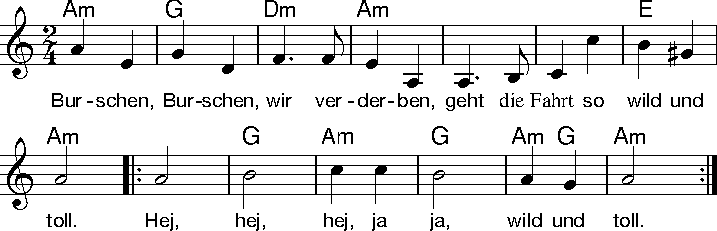
\includegraphics[draft=false, width=1\textwidth]{Noten/Lied012.pdf}

\beginverse
\[Am]Von den \[G]Füßen \[Dm]weg\[Am]gesoffen 
werden bald die \[E]Stiefel \[Am]sein,
\lrep \[Am]hej, \[G]hej, \[Am]hej, ja\[G]ja, \[Am]Stie\[G]fel \[Am]sein. \rrep
\endverse
 
\beginverse
^Eine ^Nacht, ^zwei tol^le Tage 
zechten wir an ^diesem ^Ort,
\lrep ^hej, ^hej, ^hej, ja^ja, ^die^sem ^Ort. \rrep
\endverse

\beginverse
^Zechen ^wir an ^diesem ^Orte, 
hier in diesem ^blauen ^Krug,
\lrep ^hej, ^hej, ^hej, ja^ja, ^blau^en ^Krug. \rrep
\endverse

\beginverse
^Süß das ^Bier und ^weiß ^die Kannen, 
schön die flinke ^Krüger^in.
\lrep ^hej, ^hej, ^hej, ja^ja, ^Krü^ger^in. \rrep
\endverse

\beginverse
^Sauft das ^Bier, zer^schlagt die ^Kannen, 
küsst die schöne ^Krüger^in,
\lrep ^hej, ^hej, ^hej, ja^ja, ^Krü^ger^in. \rrep
\endverse

\endsong

\beginsong{Bündische Vaganten}[
    wuw={Trenk (Alo Hamm)},
    jahr={1952},
    bo={178}, 
    pfii={27}, 
    pfiii={58}, 
    siru={96}, 
    tonspur={292}, 
    index={Hej, wie vorn der Fetzen fliegt},
]

\beginverse
\endverse
\includegraphics[draft=false, width=1\textwidth]{Noten/Lied011.pdf}

\beginverse
\[Em]Treiben wir dem \[H7]Süden zu, lässt \[Em]uns der Norden \[H7]keine Ruh',
\[Am]über\[Em]all zu \[H7]Haus' sind \[Em]wir.
Mal \[Em]rüber nach A\[H7]merika, mal \[Em]runter bis nach \[H7]Afrika,
\[Am]hoja, \[Em]hoja, \[H7]das sind \[Em]wir!
\endverse

\beginchorus 
\[C]Bündische Va\[G]ganten
\[D7]tippeln in die Welt, \[G]tippeln in die Welt.
\[C]Bündische Va\[G]ganten
\[D7]tippeln in die Welt, hei-o A\[G]yen!
\endchorus

\beginverse
^Hast du noch ein ^jung' Gesicht, so ^zage nicht und ^fack'le nicht, 
^frage ^niemals ^nach dem ^'Wie?'
Wer ^nur am Rand der ^Straße klebt, für ^seinen dummen ^Bauch nur lebt,
^misst der ^Ferne ^Zauber ^nie.
\endverse

\beginchorus
\[C]Bündische Va\[G]ganten
\[D7]tippeln in die Welt, \[G]tippeln in die Welt.
\[C]Bündische Va\[G]ganten
\[D7]tippeln in die Welt, hei-o A\[G]yen!
\endchorus

\endsong

\beginscripture{}
Vagant = Fahrendes Volk/Herumziehender; Das Lied behandelt die deutsche Jugendbewegung zwischen 1919 und 1933, die aus dem Wandervogel entstand und die Hinwendung der städtischen bürgerlichen Jugend zum Naturleben meint.
\endscripture

\beginsong{Bürgerlied}[
    mel={Prinz Eugen, der edle Ritter}, 
    meljahr={ca. 1845},
    txt={Adalbert Harnisch}, 
    txtjahr={1845}
    tonspur={432}, 
    buedel={229}, 
    gruen={188}, 
    index={Ob wir rote, gelbe Kragen},
]

\beginverse 
\endverse
\includegraphics[draft=false, width=1\textwidth]{Noten/Lied011a.pdf}

\beginverse
Ob wir \[G]können präsidieren
oder müssen Akten schmieren ohne \[D]Rast und ohne Ruh,
\lrep ob wir \[G]just Coll\[C]egia lesen
oder \[D]aber \[G]binden Besen, das tut, \[Em]das tut \[D]nichts da\[G]zu. \rrep
\endverse

\beginverse
Ob wir ^stolz zu Rosse reiten, 
oder ob zu Fuß wir schreiten barfuß ^unser'm Ziele zu,
\lrep ob uns ^Kreuze ^vorne schmücken
oder ^Kreuze ^hinten drücken, das tut, ^das tut ^nichts da^zu. \rrep
\endverse

\beginverse
Aber ^ob wir Neues bauen 
oder Altes nur verdauen, wie das ^Gras verdaut die Kuh,
\lrep ob wir ^in der ^Welt was schaffen
oder ^nur die ^Welt begaffen, das tut, ^das tut ^was da^zu. \rrep
\endverse

\beginverse
Ob im ^Kopfe etwas Grütze
und im Herzen Licht und Hitze, dass es ^brennt in einem Nu,
\lrep oder ^ob wir ^hinter Mauern
stets im ^Dunkeln ^träge kauern, das tut, ^das tut ^was da^zu. \rrep
\endverse

\beginverse
Ob wir ^rüstig und geschäftig, 
wo es gilt zu wirken kräftig, immer ^tapfer greifen zu,
\lrep oder ^ob wir ^schläfrig denken:
„Gott wird's ^schon im ^Schlafe schenken“, das tut, ^das tut ^was da^zu. \rrep
\endverse

\beginverse
D'rum, ihr ^Bürger, d'rum, 
ihr Brüder, alle eines Bundes Glieder, was auch ^jeder von uns tu'.
\lrep Alle, ^die dies ^Lied gesungen,
so die ^Alten, ^wie die Jungen: Tun wir, ^tun wir ^was da^zu! \rrep
\endverse

\endsong

\beginscripture{}
Das Lied wurde im Mai 1845 für den "Bürgerverein" der Stadt Elging geschrieben, um die Vision eines liberal gesinnten Bürgertums eines einigen deutschen Staates auszudrücken. Das Lied wurde während der Märzrevolution 1848/1849 auf Flugblättern verteilt. Nach der Revolution diente das Lied der neuen Arbeiterbewegung zum Ausdruck ihrer Forderung nach gesellschaftlicher Veränderung.
\endscripture


\setthumb{C}{3}
\beginsong{Circles}[
    mel={nach 'Windmills'},
    txt={Gwendolin Lee Zak},
    txtjahr={1979},
    bo={204}, 
    pfiii={94}, 
    siru={130}, 
    index={In days gone by},
]

\beginverse
\endverse
\includegraphics[draft=false, width=1\textwidth]{Noten/Lied013.pdf}

\beginchorus
\[G]Round and a\[D]round and a\[C]round turns the \[G]good earth;
all things must \[D]change as the \[C]seasons \[D]go \[G]by.
We are the \[D]children of the \[C]Lord and the \[G]Lady,
whose mysteries we \[D]know, but we \[C]never \[D]know \[G]why.
\endchorus

\beginverse
In \[G]all lands the \[D]people have \[C]tried to the \[G]good earth,
ploughing and \[D]sawing as the \[C]seasons \[D]de\[G]clared,
waiting to \[D]reap of the \[C]rich golden \[G]harvest,
knowing their \[D]joy in the \[C]laughs that \[D]they \[G]shared.
\endverse

\beginchorus
\[G]Round and a\[D]round and a\[C]round turns the \[G]good earth;
all things must \[D]change as the \[C]seasons \[D]go \[G]by.
We are the \[D]children of the \[C]Lord and the \[G]Lady,
whose mysteries we \[D]know, but we \[C]never \[D]know \[G]why.
\endchorus

\beginverse
Through ^Flandern and ^Wales and the ^green lands of ^Ireland,
in the kingdoms of ^England and ^Scotland ^and ^Spain,
circles grew ^up all a^long the wild ^coastlines
and worked for the ^land with the ^sun and ^the ^rain.
\endverse

\printchorus

\beginverse
^Circles for ^healing and ^working the ^weather,
circles for ^knowing the ^moon and ^the ^sun,
circles for ^thanking the ^Lord and the ^Lady,
circles for ^dancing the ^dance ne^ver ^done.
\endverse

\printchorus

\beginverse
^And we who ^reach for the ^stars in the ^heavens,
turning our ^eyes from the ^meadows ^and ^groves,
still live in the ^love of the ^Lord and the ^Lady,
the greater the ^circle, the ^more the ^love ^grows.
\endverse

\printchorus

\endsong


\setthumb{D}{4}
\beginsong{Der kleine Troll}[
    wuw={mac (Erik Martin)}, 
    bo={292}, 
    pfii={10}, 
    pfiii={40}, 
    gruen={100}, 
    siru={223}, 
    tonspur={484}, 
    index={Steigt so ein kleiner Troll},
]

\beginverse 
\endverse
\includegraphics[draft=false, width=1\textwidth]{Noten/Lied016.pdf}	

\beginverse
\[C]Plötzlich in deinem \[Am]Nacken spürst du \[G]eiskalten \[C]Hauch,
\[F]Atem des Trolls \[C]trifft dich wie \[G]giftiger \[C]Rauch.
\endverse 

\beginchorus
Sitzt du am \[F]Feuer und die \[Dm]Lieder sind ver\[G]weht, \[C]dann \[F]bleib \[G]ganz \[C]stumm,
denn in dem \[F]Land, das dich um\[Dm]gibt, ist was er\[G]wacht \[C]und \[F]schleicht \[G]he\[C]rum.
\endchorus 

\beginverse
^Du führst den Becher ^Tee nun zum Mund. ^Was zauderst ^du?
^Blütenstaub im ^Zaubertrank ^raubt dir die ^Ruh'.
\endverse

\printchorus

\newpage

\beginverse
^Wenn du in dieser ^Nacht deinen Schlaf ^findest nicht ^mehr,
^der kleine Troll ^macht uns're ^Träume so ^schwer.
\endverse

\printchorus

\endsong

\beginscripture{}
Der Autor (*1936), bekannt unter dem Fahrtennamen mac, verfasste viele bekannte Fahrtenlieder. Er beschäftigte sich intensiv mit skandinavischer Literatur und gab auch ein Jugendbuch mit dem Titel "Fjellwanderung" heraus.
\endscripture

\beginsong{Der Mond ist aufgegangen}[
    txt={Matthias Claudius}, 
    txtjahr={1779},
    mel={Johann Abraham Peter Schulz}, 
    meljahr={1790},
    pfiii={34}, 
    siru={44}, 
    tonspur={22},
]

\beginverse
\endverse 
\includegraphics[draft=false, width=1\textwidth]{Noten/Lied017.pdf}	

\beginverse
\[D]Wie \[A7]ist \[D]die \[G]Welt \[D]so \[A7]stil\[D]le und in der \[G]Dämm'\[D]rung \[A7]Höl\[D]le
so traulich \[G]und so \[A]hold! 
\[D]Als \[A7]ei\[D]ne \[G]stil\[D]le \[A7]Kam\[D]mer, wo ihr des \[G]Ta\[D]ges \[A7]Jam\[D]mer
verschlafen \[G]und \[D]ver\[A7]gessen \[D]sollt.
\endverse

\beginverse
^Seht ^ihr ^den ^Mond ^dort ^ste^hen? Er ist nur ^halb ^zu ^se^hen
und ist doch ^rund und ^schön.
^So ^sind ^wohl ^man^che ^Sa^chen, die wir ge^trost ^be^lach^en,
weil ^uns're ^Augen ^sie nicht ^seh'n.
\endverse

\beginverse
^Wir ^stol^zen ^Men^schen^kin^der sind eitel ^ar^me ^Sün^der
und wissen ^gar nicht ^viel.
^Wir ^spin^nen ^Luft^ge^spin^ste und suchen ^vie^le ^Kün^ste
und kommen ^wei^ter ^von dem ^Ziel.
\endverse

\beginverse
^Gott, ^lass ^dein ^Heil ^uns ^schau^en, auf nichts Ver^gang^lich's ^trau^en,
nicht Eitel^keit uns ^freu'n!
^Lass ^uns ^ein^fal^tig ^wer^den, und vor dir ^hier ^auf ^Er^den
wie Kinder ^fromm ^und ^fröhlich ^sein!
\endverse

\beginverse
^Wollst ^end^lich ^son^der ^Grä^men aus dieser ^Welt ^uns ^neh^men
durch einen ^sanften ^Tod.
^Und ^wenn ^du ^uns ^ge^nom^men, lass uns in ^Him^mel ^kom^men,
du unser ^Herr ^und ^unser ^Gott!
\endverse

\beginverse
^So ^legt ^euch ^denn, ^ihr ^Brü^der, in Gottes ^Na^men ^nie^der,
kalt ist der ^Abend^hauch.
^Ver^schon' ^uns, ^Gott, ^mit ^Stra^fen und lass uns ^ru^hig ^schla^fen
und unser'n ^kran^ken ^Nachbar ^auch!
\endverse

\endsong

\beginscripture{}
Dem Gedicht von Claudius als Vorlage diente~ ''Nun ruhen alle Wälder'' (1653) von Paul Gerhardt. Caulius' Gedicht enthält Reflexionen über Tod und Vergänglichkeit im Sinne christlicher Heilserwartung und könnte auch schon vor 1779 in Darmstadt entstanden sein. Seine Einfachheit wurde teilweise als naiv kritisiert, erfreute sich jedoch schnell großer Beliebtheit in der deutschen Bevölkerung.
\endscripture

\beginsong{Der Pfahl}[
    wuw={Lluís Llach}, 
    jahr={1968},
    txt={Oss Kröher},
    pfiii={56}, 
    gruen={24}, 
    siru={218}, 
    tonspur={476}, 
    buedel={278},
    index={Sonnig begann es zu tagen},
]

\beginverse
\endverse
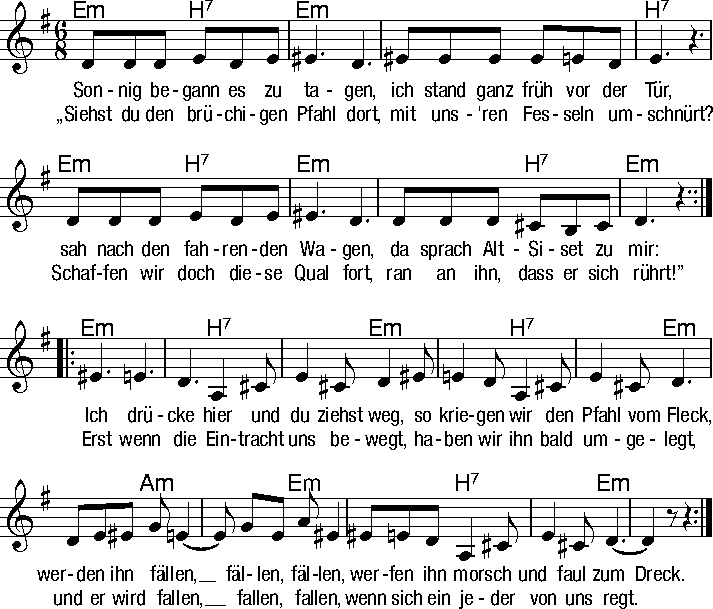
\includegraphics[draft=false, width=1\textwidth]{Noten/Lied018.pdf}	

\beginverse
\[Em]'Ach Siset, \[H7]noch ist es \[Em]nicht geschafft, an meiner Hand platzt die \[H7]Haut.
\[Em]Langsam auch \[H7]schwindet schon \[Em]meine Kraft, er ist zu \[H7]mächtig ge\[Em]baut.
Wird es uns \[H7]jemals ge\[Em]lingen? Siset, es fällt mir so \[H7]schwer!'
\[Em]'Wenn wir das \[H7]Lied nochmal \[Em]singen, geht es viel \[H7]besser. Komm \[Em]her!'
\endverse

\beginchorus 
\[Em]Ich drücke \[H7]hier und du ziehst \[Em]weg, so kriegen \[H7]wir den Pfahl vom \[Em]Fleck,
werden ihn \[Am]fällen, fällen, \[Em]fällen, werfen ihn \[H7]morsch und faul zum \[Em]Dreck.
Erst wenn die \[H7]Eintracht uns be\[Em]wegt, haben wir \[H7]ihn bald umge\[Em]legt
und er wird \[Am]fallen, fallen, \[Em]fallen, wenn sich ein \[H7]jeder von uns \[Em]regt!
\endchorus

\beginverse
^Der alte ^Siset sagt ^nichts mehr, böser Wind hat ihn ver^weht.
^Keiner weiß ^von seiner ^Heimkehr, keiner weiß, ^wie es ihm ^geht.
Alt-Siset ^sagte uns ^allen, hör es auch du, krieg es ^mit:
^Der morsche ^Pfahl wird schon ^fallen, wie es ge^schieht in dem ^Lied.
\endverse

\beginchorus
\[Em]Ich drücke \[H7]hier und du ziehst \[Em]weg, so kriegen \[H7]wir den Pfahl vom \[Em]Fleck,
werden ihn \[Am]fällen, fällen, \[Em]fällen, werfen ihn \[H7]morsch und faul zum \[Em]Dreck.
Erst wenn die \[H7]Eintracht uns be\[Em]wegt, haben wir \[H7]ihn bald umge\[Em]legt
und er wird \[Am]fallen, fallen, \[Em]fallen, wenn sich ein \[H7]jeder von uns \[Em]regt!
\endchorus

\endsong

\beginscripture{}
Das Lied ist die Übersetzung von L'Estaca von Lluís Llach. Der Pfahl steht hier sinnbildlich für das autoritäre Regime zur Zeit der Franco-Diktatur in Katalonien.
\endscripture

\beginsong{Der Piet}[
    wuw={Mac (Erik Martin)},
    jahr={1981}, 
    bo={364}, 
    pfii={69}, 
    pfiii={25}, 
    gruen={196}, 
    kssiv={46}, 
    siru={252}, 
    tonspur={570},
    index={Was kann ich denn dafür},
]

\beginverse
\endverse
\includegraphics[draft=false, width=1\textwidth]{Noten/Lied019.pdf}

\beginverse
Sie \[Am]nahmen mir die Schuh' und \[C]auch den Rock dazu.
Sie \[G]banden mir die Händ' und mein \[Am]Haus, es hat gebrennt.
Ich \[Am]sah den Galgen steh'n. Sie \[C]zwangen mich zu geh'n.
Sie \[G]wollten meinen Tod, keiner \[Am]half mir in der Not.
\endverse

\beginchorus
\lrep \[Am]Wenn der Nebel auf das \[D]Moor sich senkt, der \[F]Piet am \[G]Galgen \[Am]hängt.\rrep
\endchorus

\newpage

\beginverse
Was ^kratzt da am Genick? Ich ^spür' den rauhen Strick.
Ein ^Mönch der betet dort und spricht ^für mich fromme Wort,
die ^Wort, die ich nicht kenn', wer ^lehrte sie mich denn? 
Fünf ^Raben fliegen her, doch ich ^sehe sie nicht mehr.
\endverse

\beginchorus
\lrep \[Am]Wenn der Nebel auf das \[D]Moor sich senkt, der \[F]Piet am \[G]Galgen \[Am]hängt.\rrep
\endchorus

\endsong

\beginsong{Der Tod und der Mediziner}[
    mel={August Harder}, 
    meljahr={ca. 1810},
    txt={Gotthold Ephraim Lessing}, 
    txtjahr={1747},
    bo={168}, 
    pfii={124}, 
    pfiii={38}, 
    gruen={167a}, 
    kssiv={20}, 
    siru={89}, 
    index={Gestern Brüder könnt ihr‘s glauben},
]

\beginverse 
\endverse
\includegraphics[draft=false, width=1\textwidth]{Noten/Lied020.pdf}	

\beginverse\memorize
\[D]Drohend schwang er \[A]seine Hippe, \[D]drohend sprach das \[G]Furchtgerippe:
\[D]''Fort, du treuer \[G]Bacchusknecht! \[D]Fort, du hast ge\[A]nug ge\[D]zecht!''
\[D]''Lieber Tod'', sprach \[A]ich mit Tränen, \[D]''solltest du dich \[G]nach mir sehnen,
\[D]siehe, da steht \[G]Wein für dich. \[D]Lieber Tod, ver\[A]schone \[D]mich!''
\endverse

\beginchorus
\[D]Hopp, hopp, hopp, fa-\[A]la-la-la, ihr \[D]glaubt es nicht: Der \[A]Tod war da.
\[D]Hopp, hopp, hopp, fa-\[A]la-la-la, fa-\[D]la-la-\[A]la-la-\[D]la.
\endchorus

\beginverse
^Lächelnd greift er ^nach dem Glase, ^lächelnd trinkt er's ^aus der Base
^Auf der Pest Ge^sundheit leer, ^lächelnd stellt er's ^wieder ^her.
^Fröhlich glaubt' ich ^mich befreit, ^als er schnell sein ^Droh'n erneuert:
^''Narre, für ein ^Gläschen Wein ^denkst du'', sprach er, ^''los zu ^sein?''
\endverse

\printchorus

\beginverse
^''Tod'', sprach ich, ''ich ^möcht' auf Erden ^gern ein Medi^ziner werden.
^Lass mich, ich ver^spreche dir ^meine Kranken ^halb da^für!''
^''Gut, wenn das ist, ^magst du leben'', ^ruft er. ''Nun sei ^mir ergeben!
^Lebe, bis du ^sattgeküsst ^und des Trinkens ^müde ^bist!''
\endverse

\printchorus

\beginverse
^Oh, wie schön klingt ^das den Ohren? ^''Tod, du hast mich ^neu geboren!
^Dieses Glas voll ^Rebensaft, ^Tod, auf gute ^Brüder^schaft!''
^Ewig muss ich ^also leben, ^ewig denn dein ^Gott der Reben,
^ewig soll mich ^Lieb' und Wein, ^ewig Wein und ^Lieb' er^freu'n.
\endverse

\printchorus

\endsong

\beginsong{Der Wagen}[
    mel={Sergej Kossigin},
    meljahr={1987},
    txt={Fotler (Erik Schellhorn), Igor Plachonin},
    index={Staub, Staub und Steppenland},
    siru={222}, 
    biest={630},
    buedel={281},
]

\beginchorus
\endchorus
\includegraphics[draft=false, page=1]{Noten/Wagen-Zwischenspiel.pdf}

\beginverse
\endverse
\includegraphics[draft=false, page=1]{Noten/Wagen.pdf}

% \beginverse\memorize
% \[Am]Staub, \[F]Staub \[G]und Steppen\[Am]land,
% zwei alte \[F]Mulis\[G] am Weges\[Am]rand.
% Zieh'n den \[F]Wagen\[G] aus der \[Dm]Stadt,
% weiter nach \[Am]Osten\[E] dreht sich das \[Am]Rad.
% \endverse

\beginverse*
\nolyrics{\[F] \[G] \[Am] \[\_] \[F] \[G] \[Am] \[\_]}
\endverse

\beginverse\memorize
\[Am]Glaub', \[F]glaub', \[G] mein alter \[Am]Freund,
vom Glück da \[F]haben \[G] wir oft ge\[Am]träumt.
Knarrt das \[F]Fuhrwerk \[G] im Sturmge\[Dm]braus,
die Mulis \[Am]finden \[E] nie mehr nach \[Am]Haus.
\endverse

\beginverse*
\nolyrics{\[F] \[G] \[Am] \[\_] \[F] \[G] \[Am] \[\_]}
\endverse

\beginverse
^Fern, ^fern ^ in schwerer ^Stund',
hilft nur die ^Kneipe ^ am Wiesen^grund.
Die Wahrheit ^ände^rn wir nie^mals, 
dem Schicksal ^trotzend ^auf weiter ^Straß'.
\endverse

\beginverse*
\nolyrics{\[F] \[G] \[Am] \[\_] \[F] \[G] \[Am] \[\_]}
\endverse

\beginverse
^Weit, ^weit ^ und grau der ^Weg
und unsre ^Stiefel ^ steh'n starr vor ^Dreck.
Die Fahrt vor^bei, ^ in Träumen ^zieh'n
wir im ^Wagen ^ nochmals da^hin.
\endverse

\beginverse*
\nolyrics{\[F] \[G] \[Am] \[\_] \[F] \[G] \[Am] \[\_]}
\endverse

\beginverse
^Step, ^Step, ^ Step kru^gom,
dva starych ^mula ^ vezut fur^gon.
Iz gorodov ^ot ^ suje^ty
na Dalnij ^Zapad ^ uchodim ^my.
\endverse

\beginverse*
\nolyrics{\[F] \[G] \[Am] \[\_] \[F] \[G] \[Am] \[\_]}
\endverse

\endsong

\beginsong{Die freie Republik}[
    wuw={Studentengruppen},
    jahr={1937}, 
    bo={206}, 
    pfii={47}, 
    pfiii={23}, 
    gruen={183}, 
    kssiv={22}, 
    siru={132}, 
    tonspur={348}, 
    index={In dem Kerker saßen},
]

\beginverse
\endverse
\includegraphics[draft=false, width=1\textwidth]{Noten/Lied022.pdf}	

\beginverse
\[C]Und der Kerkermeister \[G7]sprach es täglich \[C]aus:
''Sie, Herr Bürgermeister, es \[G7]reißt mir keiner \[C]aus!''
\lrep Aber \[F]doch sind sie verschwunden abends aus dem \[C]Turm,
um die zwölfte Stunde, \[G7]bei dem großen \[C]Sturm.\rrep
\endverse

\beginverse
^Und am ander'n Morgen ^hört man den A^larm.
Oh, es war entsetzlich, ^der Soldaten^schwarm!
\lrep Sie ^suchten auf und nieder, sie suchten hin und ^her,
sie suchten sechs Studenten und ^fanden sie nicht ^mehr.\rrep
\endverse

\beginverse
^Doch sie kamen wieder, mit ^Schwertern in der ^Hand.
''Auf, auf, ihr deutschen Brüder, jetzt ^geht's für's Vater^land!
\lrep Jetzt ^geht's für Menschenrechte und für das Bürger^glück!
Wir sind doch keine Knechte der ^freien Repu^blik.''\rrep
\endverse

\beginverse
Wenn ^euch die Leute fragen: ''^Wo ist Absa^lom?''
So dürfet ihr wohl sagen: ''^Oh, der hänget ^schon.''
\lrep Er ^hängt an keinem Baume, er hängt an keinem ^Strick,
sondern an dem Glauben der ^freien Repu^blik.\rrep
\endverse


\endsong

\beginscripture{}
Erkennungslied der demokratischen Bewegung im Vormärz. Text und Melodie entstanden nach der Flucht von sechs Studenten, die am gescheiterten Frankfurter Wachensturm vom 3. April 1833 beteiligt waren. Ziel des Aufstands war die Ausrufung einer deutschen Republik durch die Besetzung der Hauptwache und Konstablerwache in Frankfurt am Main. Die Flucht der Inhaftierten gelang mit Hilfe sympathisierender Gefängniswärter. Infolge des Umsturzversuchs wurden über 1800 Personen gesucht; 39 wurden zum Tode oder zu lebenslanger Haft verurteilt.
\endscripture

\beginsong{Die Gedanken sind frei}[
    txt={Flugblätter aus Bern},
    txtjahr={ca. 1780},
    mel={aus 'Lieder der Brienzer Mädchen', ca. 1810},
    pfii={115}, 
    pfiii={31}, 
    kssiv={71}, 
    siru={52},
    tonspur={206}, 
    buedel={67}, 
]

\beginverse
\endverse
\includegraphics[draft=false, width=1\textwidth]{Noten/Lied023.pdf}

\beginverse
Ich \[G]denke, was ich will und \[D7]was mich be\[G]glücket, 
und alles in der Still', und \[D7]wie es sich \[G]schicket.
Mein \[D7]Wunsch und Be\[G]gehren kann \[D7]niemand ver\[G]wehren.
Es \[C]bleibet da\[G]bei: Die Ge\[D7]danken sind \[G]frei!
\endverse 

\beginverse
Und ^sperrt man mich ein im ^finsteren ^Kerker,
das alles sind rein ver^gebliche ^Werke,
denn ^meine Ge^danken zer^reißen die ^Schranken
und ^Mauern ent^zwei: Die Ge^danken sind ^frei!
\endverse

\beginverse
Nun ^will ich auf immer den ^Sorgen ent^sagen
und will mich auch nimmer mit ^Grillen mehr ^plagen.
Man ^kann ja im ^Herzen stets ^lachen und ^scherzen
und ^denken da^bei: Die Ge^danken sind ^frei!
\endverse

\beginverse
Ich ^liebe den Wein, mein ^Mädchen vor ^allen,
die tut mir allein am ^Besten ge^fallen.
Ich ^bin nicht al^leine bei ^einem Glas ^Weine;
mein ^Mädchen da^bei: Die Ge^danken sind ^frei!
\endverse

\endsong

\beginscripture{}
Der Text des Liedes stamm von anonymen Flugblättern aus Bern aus dem Jahr 1780. Mit Melodie wurde das Lied zuerst in der Sammlung~ ''Lieder der Brienzer Mädchen'' im frühend 19. Jahrhundert in Bern gedruckt. Zur Verbreitung trugen maßgeblich die Im Jahr 1842 veröffentlichten~ ''Schlesischen Volkslieder'' von Hoffmann von Fallersleben und Ernst Richter bei.

Das Lied diente in Zeiten politischer Unterdrückung immer wieder als Ausdruck der Sehnsucht nach Freiheit und Unabhängigkeit, so etwa während der Studentenbewegung des Vormärz, im Widerstand gegen den Nationalsozialismus oder während der Berlin-Blockade von 1948.
\endscripture

\beginsong{Die Lappen hoch}[
    wuw={Jurij Andreev, Nerother Wandervogel}, 
    jahr={1954},
    bo={78}, 
    pfii={38}, 
    pfiii={17}, 
    gruen={160}, 
    kssiv={60}, 
    siru={54},
    tonspur={212}, 
]

\beginverse
\endverse
\includegraphics[draft=false, width=1\textwidth]{Noten/Lied024.pdf}

\beginverse
Wenn \[E]einst am La\[H7]gunen\[E]rande in \[A]Lee liegt \[E]unser \[H7]Boot,
Lacht \[E]uns das \[H7]Glück am \[E]Strande, am \[A]Strande \[E]gelb und \[H7]rot.
\endverse

\beginchorus
Die Lappen \[E]hoch, die Anker \[A]fort, heute \[E]hier und \[H7]morgen \[E]dort.
\lrep Po morjam, po wol\[A]nam nietsches \[E]njet an \[H7]Safra\[E]tam.\rrep
\endchorus

\beginverse
Und nie ^würdest ^weiter du ^ziehen und ^ewig ^bliebest du ^dann,
Ja, ^wenn nicht ^wäre das ^Segeln, der ^Wind und der ^Oze^an.
\endverse

\beginchorus
Die Lappen \[E]hoch, die Anker \[A]fort, heute \[E]hier und \[H7]morgen \[E]dort.
\lrep Po moryám, po vol\[A]nám, nynche \[E]zdes nam \[H7]zavtra \[E]tam.\rrep
\endchorus

\endsong

\beginscripture{}
''Po moryám...'' bedeutet: Auf das Meer, auf die Wellen, heute hier, morgen dort.
\endscripture

\beginsong{Die Moorsoldaten}[
    mel={Rudi Goguel, Hans Eigler}, 
    meljahr={1933},
    txt={Johann Esser, Wolfgang Langhoff},
    txtjahr={1933}, 
    bo={420}, 
    pfii={68}, 
    pfiii={42}, 
    gruen={193}, 
    kssiv={72}, 
    siru={204}, 
    index={Wohin auch das Auge blicket},
]

\beginverse
\endverse
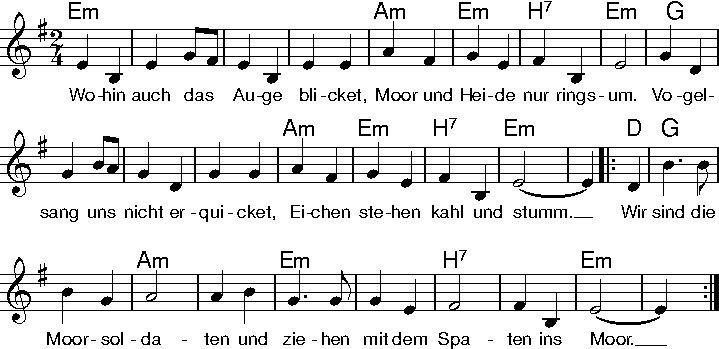
\includegraphics[draft=false, width=1\textwidth]{Noten/Lied025.pdf}	

\beginverse
\[Em]Hier in dieser öden Heide \[Am]ist das \[Em]Lager \[H7]aufge\[Em]baut,
\[G]wo wir fern von jeder Freude \[Am]hinter \[Em]Stachel\[H7]draht ver\[Em]staut.
\endverse

\beginchorus
\lrep \[D]Wir \[G]sind die Moorsol\[Am]daten und \[Em]ziehen mit dem \[H7]Spaten ins \[Em]Moor! \rrep
\endchorus

\beginverse
^Morgens ziehen die Kolonnen ^in das ^Moor zur ^Arbeit ^hin,
^Graben bei dem Brand der Sonne, ^doch zur ^Heimat ^steht der ^Sinn.
\endverse

\beginchorus
\lrep \[D]Wir \[G]sind die Moorsol\[Am]daten und \[Em]ziehen mit dem \[H7]Spaten ins \[Em]Moor! \rrep
\endchorus

\beginverse
^Heimwärts, heimwärts! Jeder sehnet ^sich nach ^Eltern, ^Weib und ^Kind.
^Manche Brust ein Seufzer dehnet, ^weil wir ^hier ge^fangen ^sind.
\endverse

\beginchorus
\lrep \[D]Wir \[G]sind die Moorsol\[Am]daten und \[Em]ziehen mit dem \[H7]Spaten ins \[Em]Moor! \rrep
\endchorus

\beginverse
^Auf und nieder geh'n die Posten; ^keiner, ^keiner ^kann hin^durch.
^Flucht wird nur das Leben kosten, ^vierfach ^ist um^zäunt die ^Burg.
\endverse

\beginchorus
\lrep \[D]Wir \[G]sind die Moorsol\[Am]daten und \[Em]ziehen mit dem \[H7]Spaten ins \[Em]Moor! \rrep
\endchorus

\beginverse
^Doch für uns gibt es kein Klagen, ^ewig ^kann's nicht ^Winter ^sein.
^Einmal werden froh wir sagen: ''^Heimat, ^Du bist ^wieder ^mein!''
\endverse

\beginchorus
\lrep \[D]Dann \[G]zieh'n die Moorsol\[Am]daten \[Em]nicht mehr mit dem \[H7]Spaten in's \[Em]Moor! \rrep
\endchorus

\endsong

\beginscripture{}
Das Lied entstand 1933 im Konzentrationslager Börgermoor (im Emsland), in dem hauptsächlich politische Gefangene untergebracht waren. Obwohl die Lagerleitung es schnell verbot, beförderte das Wachpersonal den Gesang des Liedes. Es wurde auch in anderen Moorlagern gesungen und von entlassenen Häftlingen verbreitet, sodass es sogar der Moskauer Rundfunk zu Ehren deutscher Antifaschisten spielte.
\endscripture

\beginsong{Digeding Dong Dong}

\beginverse
\endverse
\includegraphics[draft=false, width=1\textwidth]{Noten/DigedingDongDong.pdf}

\beginverse\memorize
Dige\[Em]ding dong dong, elles s'en vont à con\[D]fesse
\[Em]au curé du can\[D]ton.
\endverse

\beginverse
Dige^ding dong dong, qu'avez vous fait, les ^filles
\[Em]pour demander par\[D]don?
\endverse

\beginverse
Dige^ding dong dong, j'avions couru les ^bals
\[Em]et les jolis gar\[D]çons.
\endverse

\beginverse
Dige^ding dong dong, ma fille pour péni^tence
\[Em]nous nous embrasse\[D]rons.
\endverse

\beginverse
Dige\[Em]ding dong dong, je n'embrasse point les \[D]prêtres,
\[Em]mais les jolis gar\[D]çons
\[Em]qu'ont du poil au men\[D]ton.
\endverse

\beginverse
Dige^ding dong dong, c'est sont les filles des ^forges.
\[Em]Des forges de Paim\[D]pont.
\endverse

\endsong

\beginscripture{}
Ein traditionelles bretonisches Volkslied, das seinen Ursprung in der Region Paimpont in der Bretagne, Frankreich hat. Die erste bekannte Version des Liedes wurde im März 1872 von dem bretonischen Folkloristen Adolphe Orain im Dorf Le Cannée in der Gemeinde Paimpont gesammelt. Eine zweite Version wurde etwa 1884 von einem Schuhmacher aus Paimpont beigesteuert. Eine dritte Version wurde in den 1970er Jahren von der Gruppe Tri Yann populär gemacht und erschien 1976 auf ihrem ersten Album. \\

Übersetzung: Sie sind die Töchter der Schmiede, der Schmiede von Paimpont. / Sie gehen zur Beichte, zum örtlichen Pfarrer. /~ ''Was habt ihr Mädchen getan, um um Vergebung zu bitten?'' /~ ''Ich bin auf den Tanzbällen den hübschen Jungen nachgelaufen.'' /~ ''meine Tochter, zur Buße werden wir uns küssen.'' /~ ''Ich küsse nicht die Priester, sondern die schönen Jungen, die Haare am Kinn haben.''
\endscripture
\beginsong{Dort an dem Üferchen}[
    txt={Utta (Gustav Kemperdick)},
    mel={russische Volksweise}, 
    bo={86}, 
    pfii={41}, 
    pfiii={19}, 
    gruen={14}, 
    siru={58}, 
    tonspur={228},
]

\beginverse
\endverse
\includegraphics[draft=false, width=1\textwidth]{Noten/Lied029.pdf}	

\beginverse
\[C]Dort an dem \[G]Üferchen ent\[Am]lang dem Fluss Ka\[E]sanka 
\[F]ein gar \[G]guter \[C]Bursche ging.
Heidei, o\[G]le ole, \[Am]heidei, o\[E]le ole, 
\[F]ein gar \[G]guter \[C]Bursche ging.
\endverse

\beginverse
^Sieh, da kommt ein ^Reiter, ^führt ein ledig ^Pferd; 
der ^Bursch' be^hend hi^nauf sich schwingt.
Heidei, o^le ole, ^heidei, o^le ole, 
der ^Bursch' be^hend hi^nauf sich schwingt.
\endverse

\beginverse
^Bursch', willst du nicht ^bleiben ^bei der lieben ^Mutter 
^und dem ^greisen ^Vater dein? 
Heidei, o^le ole, ^heidei, o^le ole, 
^und dem ^greisen ^Vater dein?
\endverse

\beginverse
^Sieh, ich lieb' die ^Mutter ^und den greisen ^Vater, 
^doch die bunten ^Mützen der Ko^saken lieb ich mehr.
Heidei, o^le ole, ^heidei, o^le ole, 
^doch die bunten ^Mützen der Ko^saken lieb ich mehr.
\endverse

\beginverse
^Dort auf der ^Brücke ^steht ein junges ^Mädchen, 
^Tränen ^tropfen ^in den Fluss.
Heidei, o^le ole, ^heidei, o^le ole, 
^Tränen ^tropfen ^in den Fluss.
\endverse

\beginverse
^Dort an dem ^Üferchen, ent^lang dem Fluss Ka^sanka, 
^reiten zwei ^junge Ko^saken dahin. 
\lrep Heidei, o^le ole, ^heidei, o^le ole, 
^reiten zwei ^junge Ko^saken dahin. \rrep
\endverse


\endsong

\beginscripture{}
Die Kasanka ist ein Nebenfluss der Wolga in der Republik Tatarstan im europäischen Teil Russlands. ''Kosaken'' (bedeutet in etwa ''freie Krieger'') waren Gemeinschaften freier Reiterverbände aus flüchtigen russischen und ukrainischen Leibeigenen.
\endscripture

\beginsong{Drei glänzende Kugeln}[
    wuw={Franz Joseph Degenhardt},
    jahr={1963}, 
    bo={126}, 
    pfii={34}, 
    pfiii={15}, 
    kssiv={14}, 
    siru={74}, 
    tonspur={258}, 
    index={Es liegen drei glänzende Kugeln},
]

\beginverse
\endverse
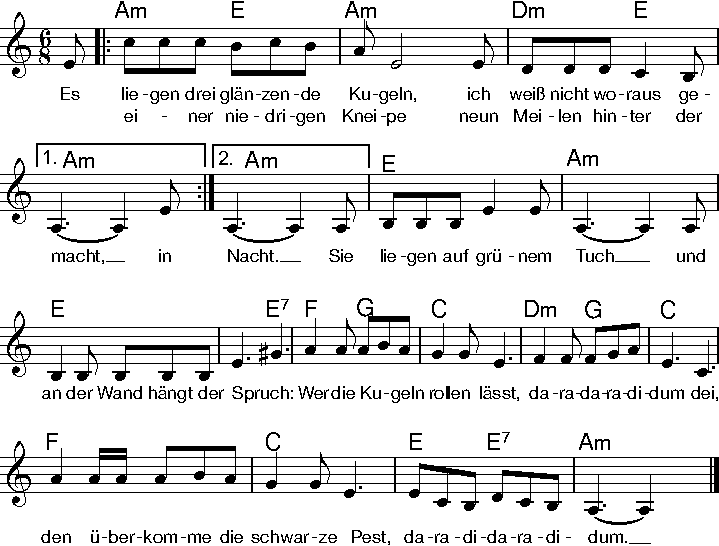
\includegraphics[draft=false, width=1\textwidth]{Noten/Lied038.pdf}	

\beginverse
Der \[Am]Wirt, der \[E]hat nur ein \[Am]Auge und \[Dm]das trägt er \[E]hinter dem \[Am]Ohr.
Aus seinem ge\[E]spaltenen \[Am]Kopfe ragt \[Dm]eine An\[E]tenne her\[Am]vor.
Er \[E]trinkt aus einer \[Am]Seele und \[E]ruft aus roter Keh\[E7]le:
\endverse

\beginchorus
\[F]Wer die Kugeln \[C]rollen lässt, \[Dm]daradaradi\[C]dum dei,
\[F]den überkomme die \[C]schwarze Pest, \[E]dara\[E7]daradi\[Am]dum.
\endchorus

\beginverse
Die ^einen ^sagen, die ^Kugeln sind die ^Sonne, die ^Erde, der ^Mond.
Die anderen ^glauben, sie ^seien das ^Feuer, die ^Angst und der ^Tod.
Und ^wenn sie beisammen ^sind, dann ^summen sie in den ^Wind:
\endverse

\beginchorus
\[F]Wer die Kugeln \[C]rollen lässt, \[Dm]daradaradi\[C]dum dei,
\[F]den überkomme die \[C]schwarze Pest, \[E]dara\[E7]daradi\[Am]dum.
\endchorus

\beginverse
Und ^dann kam ^einer ge^ritten, es ^war in dem ^Jahr vor der ^Zeit,
auf einer ^gesattelten ^Wolke von ^hinter der ^Ewig^keit.
Er ^nahm von der Wand einen ^Queue, der ^Wirt rief krächzend: ''He, ^he!''
\endverse

\printchorus

\beginverse
Doch ^jener, der ^lachte zwei ^Donner und ^wachste den ^knöchernen ^Stab,
visierte und ^stieß, und die ^Kugeln prallten ^aneinander, der ^Wirt grub sein ^Grab.
^Fäulnis flatterte ^auf, so ^nahm alles seinen ^Lauf.
\endverse

\printchorus

\endsong

\beginscripture{}
Das Lied, eines der frühesten Degenhardts, erschien erstmals auf seiner Platte "Zwischen Null Uhr Null und Mitternacht" (1963). Ein Interpretationsansatz geht davon aus, dass in dem Lied das Forschen mit Atomenergie kritisiert wird. So könnten die Kugeln für die Atome stehen, die vom Menschen nicht angestoßen werden sollen, und der verunstaltete Wirt für die möglichen gesundheitlichen Folgen des Experimentierens mit Atomenergie.
\endscripture

\beginsong{Drei rote Pfiffe}[
    txt={Heinz Rudolf Unger}, 
    mel={Georg Herrnstadt, Wilhelm Resetarits},
    jahr={1979}, 
    bo={198},
    siru={124},
    tonspur={340},
    index={Im Kreis ihrer Enkel, die alte Frau},
]

\beginverse
\endverse
\includegraphics[draft=false, width=1\textwidth]{Noten/Lied030.pdf}	

\beginverse
Die \[D]Drau hinunter trieb Mond um Mond, es \[Hm]brach der Faschistenkrieg aus.
Da \[F\#m]hatte ich einen \[G]Mann an der Front und \[Hm]hatte drei Kinder im \[A]Haus,
und hatte drei Kinder im \[D]Haus.
Wie \[Hm]tönte da markiger Nazigesang von \[A]deutschem Boden und Blut.
\[G]Manch ein Bursch' in die \[D]Berge entsprang, ich trug \[F\#m]Flugblätter unter dem Hut,
ich trug \[G]Flugblätter unter dem \[D]Hut.
Der \[D]Gestapo war kalt und der Gauleiter schalt: Parti\[Hm]sanen im eigenen Land!
Ich \[F\#m]trug das Geflüster und \[G]Brot in den Wald. Sie \[Hm]haben mich Jelka ge\[A]nannt.
Sie haben mich Jelka ge\[D]nannt.
\endverse

\beginchorus
Ver\[Dm]schwiegene Bäume, ver\[B]schworener Wald
Und \[F]drei rote Pfiffe, \[Am]drei rote Pfiffe, \[B]drei rote \[Gm]Pfiffe im \[D]Wald.
\endchorus

\beginverse
Der ^Winter war nass und uns wärmte der Hass, viele ^sind's, die die Erde heut' birgt. Wir ^haben gefochten, dort ^oben am Pass, an ^uns'rer Befreiung ge^wirkt,
an uns'rer Befreiung ge^wirkt.
Der ^Krieg war vorbei, da war Stille im Land, da ^waren die Lautesten leis'.
Sie ^nahmen das Hitler^bild von der Wand, ihre ^Westen, die wuschen sie weiß,
ihre ^Westen, die wuschen sie ^weiß.
^Ihr, meine Enkel, was hört ihr so stumm die ^alten, die kalten Berichte?
Jetzt ^trampeln sie wieder auf euren ^Rechten herum, er^innert euch meiner Ge^schichte, erinnert euch meiner Ge^schichte.
\endverse

\printchorus

\endsong

\beginscripture{}
% Siehe Seite 160
\endscripture


\setthumb{E}{5}
\beginsong{Edelweißpiraten}[
    wuw={Herwig Steymans, Hans-Jörg Maucksch}, 
    bo={280}, 
    pfii={70}, 
    pfiii={26}, 
    siru={209}, 
    tonspur={466}, 
    index={Sie saßen oft am Märchensee},
]

\beginverse
\[G] Sie saßen \[Hm]oft beim Märchen\[C]see am Lager\[G]feuer, \[Em] sie wollten \[Am]leben, wie es \[D]ihnen ge\[G]fiel. Der neue \[Hm]Kurs im deutschen \[C]Land war nicht ge\[G]heuer, \[Em] sie wollten \[Am]frei sein mit Ge\[D]sang, Gitarren\[G]spiel.
\[D] Mit ihrer \[C]Kleidung nahmen \[G]sie's nicht so ge\[D]nau. Ganz offen \[C]trugen sie das \[G]Edelweiß zur \[D]Schau, und das war \[C]gut, sie hatten \[G]Mut.
\endverse

\beginverse
\[G] Sie hielten \[Hm]nichts von den \[C]braunen Nazi\[G]horden, \[Em] sie hielten \[Am]nichts von dem Ge\[D]schrei nach Heil und \[G]Sieg. Was war denn \[Hm]bloß aus ihrem \[C]Vaterland ge\[G]worden? \[Em] Man schürte \[Am]offen den ver\[D]brecherischen \[G]Krieg.
\[D] Da gab's nur \[C]eins zu tun: Be\[G]frei'n wir dieses \[D]Land! Da durfte \[C]keiner ruh'n, wir \[G]leisten Wider\[D]stand! Sie hatten \[C]Mut und das war \[G]gut.
\endverse

\beginchorus
\lrep Vielleicht wird \[D]morgen schon \[Am] eine neue \[C]Zeit anfangen,
\[G] vielleicht ist \[D]morgen schon \[C] der Spuk vor\[G]bei. \rrep
\endchorus

\beginverse
^ Da gab's 'nen ^Güterzug mit ^Kriegsgerät und ^Waffen ^ und was man ^sonst noch braucht für ^einen Völker^mord. Da machten ^sie sich an den ^Gleisen kurz zu ^schaffen, ^ der Zug er^reichte niemals ^den Bestimmungs^ort.
^ Und Essens^marken aus dem ^Parteibüro der ^Stadt war'n plötzlich ^weg und Zwangsar^beiter wurden ^satt, und das war ^gut, und das war ^gut.
\endverse

\beginverse
^ Sie glaubten ^fest daran, dass ^sie den Sieg er^ringen, ^ sie glaubten ^fest daran, aus ^Schaden wird man ^klug. Sie glaubten ^fest daran, als ^sie zum Galgen ^gingen, ^ sie glaubten ^fest daran, als ^man sie vorher ^schlug.
^ Und dann die ^Angst, die vor ^jeder Folter ^steht, die ist so ^groß, dass man den ^besten Freund ^verrät, versteht man ^gut, versteht man ^gut.
\endverse

\beginverse
^ Sie stehen ^heute noch auf ^manchen schwarzen ^Listen, ^ ich würd' fast ^sagen, es ist ^wieder mal so^weit. In Amt und ^Würden sitzen ^immer noch Fa^schisten ^ und zum to^talen Krieg ist ^mancher schnell be^reit.
^ Doch seh' ich ^Tausende, und ^das beruhigt mich ^sehr, die zeigen ^offen das zer^brochene Ge^wehr, und das macht ^Mut, und das macht ^Mut.
\endverse

\beginchorus
\lrep Und dann wird \[D]morgen schon \[Am] eine neue \[C]Zeit anfangen
\[G] und dann ist \[D]morgen schon \[C] der Spuk vor\[G]bei. \rrep
\endchorus

\endsong

\beginscripture{}
Die Edelweißpiraten waren eine Gruppe Jugendlicher zur Zeit des Dritten Reichs, die sich der Hitlerjugend nicht anschließen wollten. Als sie weiterhin auf Fahrten gingen, wurden sie von der Gestapo verfolgt und wurden oppositionell politisch. Bis zuletzt wurden Edelweißpiraten, die an einem Abzeichen erkennbar waren, verfolgt und erschossen. Bis heute sind sie nicht als Widerstandsgruppe anerkannt. Dieses Lied reflektiert besonders die Bedeutung der Ehrenfelder Gruppe.
\endscripture

\beginsong{Ein Hotdog unten am Hafen}[
    wuw={Element of Crime}, 
    alb={Robert\\ Zimmermann wundert sich über die Liebe}, 
    jahr={2008}, 
    siru={66}, 
    biest={546},
]

% \beginverse\memorize
% Ein \[Am]Hotdog unten am \[C]Hafen und vor'm \[E]Einschlafen schnell noch ein \[F]Bier,
% dem \[C]Feind einen Tritt in die \[F]Rippen und ein paar \[G]Kippen für hinterher.
% Ein \[Am]Date mit dem Dalai La\[C]ma und ein \[E]Apfelsaft morgens um \[F]zwei
% und eine \[C]halbautomatische \[G]Waffe ist immer da\[C]bei.
% \endverse
%
% \beginchorus
% \[Am]Schön, wenn man liebt, was \[Em]Mutter Natur einem gibt.
% Was kann \[F]ich dafür, dass \[G]du mich nicht ver\[C]gisst?
% Ein ge\[F]selliges Tier ist das \[G]Schwein, und das \[C]Stachelschwein lieber al\[Am]lein.
% \[C]Ohne dich will ich nicht, \[G]mit dir kann ich nicht \[C]sein.
% \endchorus

\includegraphics[draft=false, width=1\textwidth]{Noten/EinHotdogUntenAmHafenV.pdf}

\beginverse
\endverse

\beginverse
\[Am]Räucherstäbchen und \[C]Wildreis und \[E]Abende auf dem Bal\[F]kon,
in \[C]Eppendorf ist morgen \[F]Flohmarkt und \[G]jeder nach seiner Facon.
Ein \[Am]Date mit dem Dalai La\[C]ma und ein \[E]Griff ins Kosmetikre\[F]gal,
und wenn's im \[C]Rücken mal weh tut wird \[G]jede Bewegung zur \[C]Qual.
\endverse

\beginchorus
\[Am]Schön, wenn man liebt, was \[Em]Mutter Natur einem gibt.
Was kann \[F]ich dafür, dass \[G]du mich nicht ver\[C]gisst?
Ein ge\[F]selliges Tier ist das \[G]Schwein, und das \[C]Stachelschwein lieber al\[F]lein.
\[C]Ohne dich will ich nicht, \[G]mit dir kann ich nicht \[C]sein.
\endchorus

\beginverse\memorize
Eine ^Parkbank in Planten un ^Blomen und der ^Mond über Altona,^
einen ^Sohn, der bald mal ins ^Bett muss, und ^trockene Blumen im Haar.
Ein ^Date mit dem Dalai La^ma und ein ^Klimpern auf dem Kla^vier
und zum ^Abschied ein bisschen Ge^fummel hinter der ^Tür.
\endverse

\beginchorus
\[Am]Schön, wenn man liebt, was \[Em]Mutter Natur einem gibt.
Was kann \[F]ich dafür, dass \[G]du mich nicht ver\[C]gisst?
Ein ge\[F]selliges Tier ist das \[G]Schwein, und das \[C]Stachelschwein lieber al\[F]lein.
\[C]Ohne dich will ich nicht, \[G]mit dir kann ich nicht \[C]sein. \[G]
\[C]Ohne dich will ich nicht, \[G]mit dir kann ich nicht \[C]sein.
\endchorus

\endsong
\input{Lieder/EinKrampenschlagvorTag}
\input{Lieder/EinstolzesSchiff}
\beginsong{Es ist an der Zeit}[
    wuw={Eric Bogle},
    jahr={1976},
    txt={Hannes Wader (Übersetzung)},
    txtjahr={1980)}, 
    pfii={86},
    pfiii={43}, 
    gruen={199}, 
    biest={644},
    siru={259}, 
    tonspur={584}, 
    index={Weit in der Champagne},
]

\beginverse
Weit \[G]in der Cham\[Em]pagne im \[C]Mittsommer\[Am]grün,
dort \[D]wo zwischen Grabkreuzen \[G]Mohnblu\[C]men \[G]blüh'n.
Da \[G]flüstern die \[Em]Gräser und \[C]wiegen sich \[Am]leicht
im \[D]Wind, der sanft über das \[G]Gräber\[D7]feld \[G]streicht.
Auf \[G]deinem Kreuz \[Em]finde ich \[Am]toter Soldat
deinen \[D]Namen nicht, nur Ziffern \[G]und jemand \[D]hat
die \[G]Zahl Neunzehn\[Em]hundertund\[Am]sechzehn ge\[C]malt
und du \[D]warst nicht einmal neunzehn \[G]Jah\[D7]re \[G]alt.
\endverse

\beginchorus
Ja, auch \[D]dich haben sie schon ge\[C]nauso be\[G]logen,
so, wie \[D]sie es mit uns heute \[C]immer noch \[G]tun,
und du \[C]hast ihnen alles ge\[D]geben:
Deine \[G]Kraft, deine \[C]Jugend, dein \[D]Le\[G]ben.
\endchorus

\beginverse\memorize
Hast du, \[G]toter Sol\[Em]dat, mal ein \[C]Mädchen ge\[Am]liebt?
Sicher \[D]nicht, denn nur dort, wo es \[G]Frie\[C]den \[G]gibt,
können \[G]Zärtlichkeit \[Em]und Ver\[C]trauen ge\[Am]deih'n.
Warst \[D]Soldat, um zu sterben, nicht \[G]um jung \[D7]zu \[G]sein.
Viel\[G]leicht dachtest \[Em]du dir: Ich \[Am]falle schon bald,
nehme \[D]mir mein Vergnügen, wie es \[G]kommt, mit Ge\[D]walt.
Dazu \[G]warst du ent\[Em]schlossen, hast \[Am]dich aber \[C]dann
vor dir \[D]selber geschämt und es \[G]doch nie \[D7]ge\[G]tan.
\endverse

\printchorus

\beginverse
Sol^dat, gingst du ^gläubig und ^gern in den ^Tod?
Oder ^hast du verzweifelt, ver^bittert, ^ver^roht
deinen ^wirklichen ^Feind nicht er^kannt bis zum ^Schluss?
Ich ^hoffe, es traf dich ein ^saube^rer ^Schuss.
Oder ^hat ein Ge^schoss dir die ^Glieder zerfetzt?
Hast du ^nach deiner Mutter ge^schrien bis zu^letzt?
Bist du ^auf deinen ^Beinstümpfen ^weiterge^rannt?
Und dein ^Grab, birgt es mehr als ein ^Bein, ei^ne ^Hand?
\endverse

\printchorus

\beginverse
Es ^blieb nur das ^Kreuz als die ^einzige ^Spur
^von deinem Leben, doch ^hör' mei^nen ^Schwur
für den ^Frieden zu ^kämpfen und ^wachsam zu ^sein.
Fällt die ^Menschheit noch einmal auf ^Lügen ^he^rein,
dann ^kann es ge^scheh'n, dass bald ^niemand mehr lebt,
niemand, ^der die Milliarden von ^Toten be^gräbt.
Doch längst ^finden sich ^mehr und mehr ^Menschen be^reit,
diesen ^Krieg zu verhindern, es ^ist an ^der ^Zeit.
\endverse

\printchorus

\endsong

\beginscripture{}
Das Lied ist die deutsche Variante von ''The green fields of France'' von Eric Bogle und wurde in dieser Version zu einer Hymne der Friedensbewegung in den 1980er Jahren.
\endscripture

\beginsong{Es soll sich der Mensch}[
    txt={nach den 'Hayner Dorfmusikanten'},
    txtjahr={um 1800},
    mel={Fiedel Michel},
    meljahr={1978}, 
    bo={130}, 
    pfii={82}, 
    pfiii={44}, 
    siru={76},
    tonspur={262}, 
]

\beginverse
\endverse
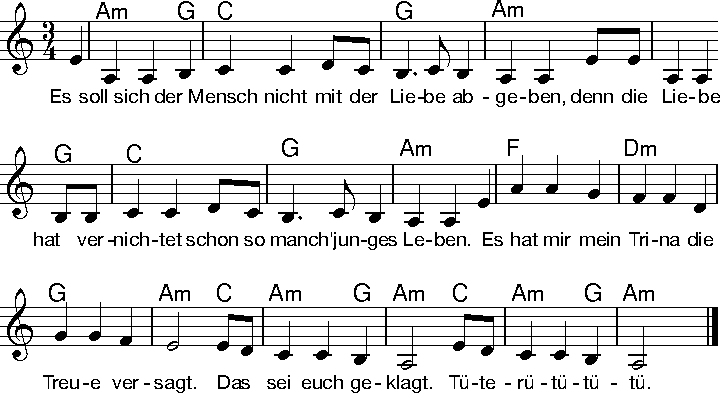
\includegraphics[draft=false, width=1\textwidth]{Noten/Lied039.pdf}	

\beginverse
Ich \[Am]war ja \[G]so \[C]schrecklich in die \[G]Trina ver\[Am]schossen;
mein Herz war \[G]mit \[C]Zucker und mit \[G]Honig über\[Am]gossen.
Da \[F]kommt doch, zum \[Dm]Teufel, dem \[G]Müller sein \[Am]Franz
\[C]und der \[Am]führt sie \[G]zum \[Am]Tanz. \[C]Tü-te-\[Am]rü-tü-\[G]tü-\[Am]tü.
\endverse

\beginverse
Und nun ^schmeckt mir ^kein ^Essen und es ^schmeckt mir kein ^Trinken.
Am liebsten ^da ^würd' ich in der ^Erde ver^sinken.
Ich ^geh auch nicht ^mehr mit die ^anderen ^Knechte,
^denn die ^Menschen ^sind ^schlechte. ^Tü-te-^rü-tü-^tü-^tü.
\endverse

\beginverse
Und ^sollt' man ^mit ^solch' Mädchen zum ^Tanze aus^gehen,
ja, dann bleibt man ^am ^besten ganz ^dicht dabei ^stehen,
denn ^sonst tanzen sie ^gleich mit die ^anderen ^Knechte,
^denn solch ^Mädchen ^sind ^schlechte. ^Tü-te-^rü-tü-^tü-^tü.
\endverse

\beginverse
Und ^bin ich ^ge^storben, so ^lasst mich be^graben
und lasst mir ^beim ^Schreiner sechs ^Bretter ab^schaben.
Da^rauf dann zwei ^feurige ^Herzen lasst ^malen,
^denn ich ^kann's ja ^be^zahlen. ^Tü-te-^rü-tü-^tü-^tü.
\endverse

\beginverse
Und ^dann sollt ^ihr ^ein feierlich ^Totenlied ^singen:
Da liegt nun ^der ^Esel in die ^Quer und die ^Längen.
Er ^hat sich ver^plempert mit ^Liebesaf^fären:
^Zu ^Dreck soll ^er ^werden! ^Tü-te-^rü-tü-^tü-^tü.
\endverse

\beginverse
So ^ging das ^zwei ^Wochen und dann ^kam schon die ^Nächste;
vergessen ^all  die ^Sorgen, die ^Ängste, die ^Nöte.
Da ^fing das The^ater von ^vorne ^an;
^man ge^wöhnt sich ^da^ran! ^Tü-te-^rü-tü-^tü-^tü.
\endverse

\endsong

\beginscripture{}
Die 7. Strophe ist aus dem Mittelfränkischen entlehnt und wurde später hinzugefügt.
\endscripture

\beginsong{Es war an einem Sommertag}[
    wuw={Arno Clauss}, 
    jahr={1973},
    bo={136}, 
    pfii={88}, 
    pfiii={36}, 
    gruen={176}, 
    kssiv={26}, 
    siru={78},
    tonspur={265}, 
]

\beginverse
\endverse
\includegraphics[draft=false, width=1\textwidth]{Noten/Lied040.pdf}	

\beginverse
Ein \[C]Mann mit \[G]einem \[C]Feder\[G]hut rief: ''\[Am]Männer, \[E]hört mir \[Am]zu!
\[C]Ich ver\[G]sprech' euch \[C]Geld und Gut \[G]und \[Am]Ehre \[E]noch da\[Am]zu.
Der \[G]Kaiser braucht euch, \[C]reiht euch ein, denkt \[G]nicht an Weib und \[C]Haus!
Es \[G]muss ja nicht für \[C]lange sein, zieht \[Am]mit ins \[E]Feld hi\[Am]naus!''
{\nolyrics \[C] \[G] \[C] \[G] \[Am] \[E] \[Am]}
\endverse

\beginverse
Im ^Wirtshaus ^war das ^Trinken ^frei, bezahlt ^mit des ^Kaisers ^Gold.
Und ^während ^dieser ^Zeche^rei trat ^mancher in des ^Kaisers ^Sold.
Gab ^seiner Braut den ^Abschiedskuss, ver^suchte als Soldat sein ^Glück,
Sah ^nicht des Werbers ^Pferdefuß und ^kam nicht ^mehr zu^rück.
{\nolyrics \[C] \[G] \[C] \[G] \[Am] \[E] \[Am]}
\endverse

\beginverse
Mit ^Flöten^spiel und ^Trommel^schlag ging's ^früh am ^Morgen ^fort.
Die ^Schar ward ^größer, ^denn es ^lag am ^Weg noch ^mancher ^Ort.
Der ^Werber mit dem ^Federhut macht' ^sein Geschäft nicht ^schlecht,
ver^sprach noch vielen ^Geld und Gut, dem ^Kaiser ^dem war's ^recht.
{\nolyrics \[C] \[G] \[C] \[G] \[Am] \[E] \[Am]}
\endverse

\beginverse
Die ^Jahre ^gingen ^in das ^Land und ^von der ^großen ^Schar
war ^keiner, ^der nach ^Hause ^fand, wie ^er ge^gangen ^war.
Der ^eine ließ sein ^Bein im Feld, blind ^kam ein and'rer ^an.
Die ^meisten hatte der ^Tod gefällt, der ^jede ^Schlacht ge^wann.
{\nolyrics \[C] \[G] \[C] \[G] \[Am] \[E] \[Am]}
\endverse

\beginverse
Die ^letzten ^Tränen ^waren ^kaum ge^weint, da ^waren ^sie
auch ^schon ver^gessen, ^wie ein ^Traum; die ^Menschen ^lernen ^nie!
Und ^dann an einem ^Sommertag, irgend^wann und irgend^wo,
da ^tönte wieder ^Trommelschlag, und ^Flöten^spiel klang ^froh.
{\nolyrics \[C] \[G] \[C] \[G] \[Am] \[E] \[Am]}
\endverse

\endsong

\beginsong{Es wollt' ein Bauer früh aufsteh'n}[
    wuw={Volkslied aus dem 15. Jahrhundert},
    mel={Zupfgeigenhansel},
    meljahr={1976},
    bo={142}, 
    pfii={76}, 
    pfiii={57}, 
    gruen={147},
]

\beginverse
\endverse
\includegraphics[draft=false, width=1\textwidth]{Noten/Lied042.pdf}

\beginverse
Und \[D]als der Bauer nach Hause kam, und als der Bauer nach \[A]Hause kam,
da wollt er was zu \[D]fressen ham'. \[A]Fal-te-rie-te-\[D]ra-la-la, \[A]fal-te-rie-te-\[D]ra.
\endverse

\beginverse
Ach ^Lieschen, koch mir Hirsebrei, ach Lieschen, koch mir ^Hirsebrei
mit Bratkartoffeln, ^Spiegelei! ^Fal-te-rie-te-^ra-la-la, ^fal-te-rie-te-^ra.
\endverse

\beginverse
Und ^als der Bauer saß und fraß, und als der Bauer ^saß und fraß,
da rumpelt in der ^Kammer was.  ^Fal-te-rie-te-^ra-la-la, ^fal-te-rie-te-^ra.
\endverse

\beginverse
Ach ^liebe Frau, was ist denn das? Ach liebe Frau, was ^ist denn das?
Da rumpelt in der ^Kammer was. ^Fal-te-rie-te-^ra-la-la, ^fal-te-rie-te-^ra.
\endverse

\beginverse
Ach ^lieber Mann, das ist der Wind, ach lieber Mann, das ^ist der Wind,
der raschelt da im ^Küchenspind. ^Fal-te-rie-te-^ra-la-la, ^fal-te-rie-te-^ra.
\endverse

\beginverse
Der ^Bauer sprach: Will selber seh'n. Der Bauer sprach: Will ^selber seh'n,
will selber in die ^Kammer geh'n.  ^Fal-te-rie-te-^ra-la-la, ^fal-te-rie-te-^ra.
\endverse

\beginverse
Und ^als der Bauer in d' Kammer kam, und als der Bauer in d' ^Kammer kam,
da zog der Pfaff' die ^Hosen an.  ^Fal-te-rie-te-^ra-la-la, ^fal-te-rie-te-^ra.
\endverse

\beginverse
Ei ^Pfaff', was machst in meinem Haus? Ei Pfaff', was machst in ^meinem Haus?
Ich werf dich ja so^gleich hinaus. ^Fal-te-rie-te-^ra-la-la, ^fal-te-rie-te-^ra.
\endverse

\beginverse
Der ^Pfaff', der sprach: Was ich verricht', der Pfaff, der sprach: Was ^ich verricht',
dein' Frau, die kann die ^Beicht noch nicht.  ^Fal-te-rie-te-^ra-la-la, ^fal-te-rie-te-^ra.
\endverse

\beginverse
Da ^nahm der Bauer ein' Ofenscheit, da nahm der Bauer ein' ^Ofenscheit
und schlug den Pfaffen, ^dass er schreit. ^Fal-te-rie-te-^ra-la-la, ^fal-te-rie-te-^ra.
\endverse

\beginverse
Der ^Pfaffe schrie: O Schreck, o Graus!, der Pfaffe schrie: O ^Schreck, o Graus!
und hielt den Arsch zum ^Fenster raus. ^Fal-te-rie-te-^ra-la-la, ^fal-te-rie-te-^ra.
\endverse

\beginverse
Da ^kamen die Leut' von nah und fern, da kamen die Leut' von ^nah und fern
und dachten, es sei der ^Morgenstern. ^Fal-te-rie-te-^ra-la-la, ^fal-te-rie-te-^ra.
\endverse

\beginverse
Der ^Morgenstern, der war es nicht, der Morgenstern, der ^war es nicht,
es war des Pfaffen ^Arschgesicht. ^Fal-te-rie-te-^ra-la-la, ^fal-te-rie-te-^ra.
\endverse

\beginverse
So ^soll es allen Pfaffen geh'n, so soll es allen ^Pfaffen geh'n,
die nachts zu fremden ^Weibern geh'n. ^Fal-te-rie-te-^ra-la-la, ^fal-te-rie-te-^ra.
\endverse

\beginverse
Und ^die Moral von der Geschicht', und die Moral von ^der Geschicht':
Trau' nicht des Pfaffen ^Arschgesicht! ^Fal-te-rie-te-^ra-la-la, ^fal-te-rie-te-^ra.
\endverse

\endsong

\beginscripture{}
Pfaffe ist ein wenig gebrauchtes Wort für einen Pfarrer beziehungsweise einen Geistlichen.
\endscripture


\setthumb{F}{6}
\beginsong{Frühling dringt in den Norden}[
    wuw={Mayer (Jürgen Sesselmann), Nerother Wandervogel},
    jahr={1980, 5. Strophe: 2017}, 
    kssiv={44}, 
    siru={86}, 
    bo={160},
    tonspur={276}, 
]

\beginverse
\endverse
\includegraphics[draft=false, page=1]{Noten/FruehlingDringtInDenNorden.pdf}

\beginverse\memorize
\[Em]Sommer \[D]er\[G]füllt \[D]den \[G]Norden, 
Mücken \[D]sind zur \[C]Plage \[D]nun ge\[Em]worden.
In den Höhen \[G]kreist der Greif,
\[C]Lachse ziehn'n zum Laichen \[G]auf \[C]bis ans Ziel und sterben \[G]drauf.
\[C]Lichter \[G]Tag nicht \[Am]enden \[Em]mag im \[C]Sommer \[D]hoch im \[Em]Norden. \[G]\[D]\[Em]
\endverse

\beginverse
^Herbstzeit ^durch^jagt ^den ^Norden, 
erste ^Nächte sind ^frostig ^kalt ge^worden.
Stürme zerr'n an ^gelbem Laub,
^reife Früchte prahlen ^bunt. ^Bären schwelgen sich dran ^rund,
^gegen ^Süd die ^Graugans ^zieht zur ^Herbstzeit ^hoch im ^Norden. ^^^
\endverse

\beginverse
^Winter ^be^herrscht ^den ^Norden, 
alle ^Wasser sind ^zu Kris^tall ge^worden.
Wölfe heulen ^fern im Tal.
^Lange Zeit Schneekönig ^Mond ^über'm Land alleine ^trohnt
^wie ein ^Spuk der ^Nordlicht ^Flug im ^Winter ^hoch im ^Norden. ^^^
\endverse

\beginverse
^Füllt neu ^der ^Lenz ^den ^Norden,
sind die ^Blüten ^ihm zu^teilge^worden.
Eis treibt schmelzend ^mit dem Strom.
^Abermals die Vögel ^dann ^künden laut den Frühling ^an.
^Jung durch's ^Grün die ^Elche ^zieh'n, im ^nächsten ^Lenz im ^Norden. ^^^
\endverse

\endsong

\beginscripture{}
\begin{tabularx}{1\textwidth}{@{}X@{}}
Mayer, mit bürgerlichem Namen Jürgen Sesselmann, ist Teil der Nerother Wandervogel, Orden der Bockreiter. Das Lied stammt aus Mayers Nordamerikazyklus und ist im Herbst 1980 am Yukon River entstanden. Die fünfte Strophe schrieb er erst 2017 dazu.
\end{tabularx}
\endscripture


\setthumb{G}{7}
\beginsong{Geburtstagslied}[
    wuw={Aleksander Timofejewski},
    jahr={1971},
    txt={Erik Schellhorn (Übersetzung), letzte Strophe aus studentischen Kreisen},
    txtjahr={1991},
    bo={278}, 
    siru={207}, 
    tonspur={460}, 
    index={Seht die Leute, sie springen ungeschickt über Pfützen},
]

\beginverse
\endverse
\includegraphics[draft=false, width=1\textwidth]{Noten/Lied046.pdf}	


\beginverse
Plötzlich \[Am]kommt ein Hubschrauber
und he\[E]raus steigt ein Zaub'rer,
zeigt den Film “Pippi geht auf die \[Am]Walz”.
Zum Ge\[A]burtstag, da wünscht
er mir viel \[Dm]Glück und wie immer
schenkt er \[Am]mir eine \[E]Tonne voll \[Am]Eis.
\endverse

\beginchorus
Und doch, ich \[E]spiele auf der Ga\[Am]moschka,
man sieht mich \[G]auf dem Trotto\[C]ir.
\lrep Aber \[Dm]leider ist Ge\[Am]burtstag
nur ein\[Dm]mal \[E7]im \[Am (A7)]Jahr. \rrep
\endchorus

\beginverse
Ich hab' ^heute Geburtstag,
alle ^kommen am Sonntag,
fröhlich lärmen sie im Haus he^rum.
Und sie ^tanzen, sie singen,
dass die ^Wände mitschwingen,
und zer^stören mein ^Aquari^um.
\endverse

\beginchorus
Oh, wie sie \[E]rauchen und sie ver\[Am]sauen
den Teppich, \[G]der ganz neu noch \[C]war.
\lrep Ach, wie \[Dm]gut, man hat Ge\[Am]burtstag
nur ein\[Dm]mal \[E7]im \[Am (A7)]Jahr. \rrep
\endchorus

\endsong

\beginscripture{}
Dies ist die Übersetzung des ''Liedes des Krokodils Gena'', einer russischen Roman-, Theater- und Zeichentrickfilmfigur.
\endscripture

\beginsong{Gospodar}[
    mel={Rudi Rogoll, 1984}, 
    txt={Theodor Kramer, 1984}, 
    bo={172}, 
    pfiii={64}, 
    siru={90},
    tonspur={284}, 
]

\beginverse
\endverse
\includegraphics[draft=false, width=1\textwidth]{Noten/Lied047.pdf}	

\beginverse
\[Am]Treiben wir die \[Dm]Fremden \[Am]über's \[E]Jahr erst \[Am]aus.
\[C]Gospodar, wer glaubst du, \[G]bleibt im Herrschafts\[C]haus?
\lrep \[Am]Werd' ich knechtisch \[Dm]aufsteh'n, \[G7]wo ich mächtig \[C]sitz'?
\[Am]Sind nicht solche \[Dm]Tölpel, \[Am]Bruder \[E]Sliwo\[Am]witz.\rrep
\endverse

\beginverse
^Haben unser ^Herzblut ^nicht für ^nichts ver^tan.
^Alles für die Seinen ^will der Parti^san:
\lrep ^Mutterschaf und ^Lämmer, ^Gänse, Geiß und ^Kitz,
^Kürbis und Me^lonen, ^Mais und ^Sliwo^witz.\rrep
\endverse

\beginverse
^Sind die wilden ^Schweine ^aus dem ^Land ver^jagt,
^die verkohlten Hütten ^aufgebaut und ^ragt
\lrep ^blank im Dorf der ^Maibaum, ^Flattern und Ge^fitz;
^oh, wie wird das ^schön sein, ^Bruder ^Sliwo^witz.\rrep
\endverse

\endsong

\beginscripture{}
Partisanen = Bewaffnete Widerstandskämpfer, die im eigenen Land gegen eine Besatzungsmacht, ein autoritäres Regime oder fremde Truppen kämpfen.
Besonders während der Besetzung durch die Achsenmächte im Zweiten Weltkrieg spielten Partisanen eine bedeutende Rolle im Widerstand.

Gospodar kommt aus dem slawischen und bedeutet Gaststätte. Sliwowitz ist ein in Osteuropa verbreiteter Pflaumenbranntwein.
\endscripture

\beginsong{Gregor}[
    txt={aus der Jungenschaft, niedergeschrieben von Eberhard Köbel und Günther Wolff}, 
    txtjahr={1934}, 
    mel={nach ukrainischem Volkslied}, 
    bo={166},  
    pfii={104}, 
    pfiii={65}, 
    kssiv={40}, 
    siru={87}, 
    tonspur={278}, 
    index={Gehe nicht, oh Gregor},
]

\beginverse
\endverse
\includegraphics[draft=false, width=1\textwidth]{Noten/Lied048.pdf}	

\beginverse
\[Dm]Dort ist auch die eine mit den \[A7]schwarzen Augen\[Dm]brauen.
Glaube mir, oh Gregor, das ist \[A7]eine Zaube\[Dm]rin. \[C]
\lrep \[F]Ihre schmale Hand braut dir \[C]Tee aus Zauber\[F]kräu\[A7]tern,
\[Dm]legt sich über deine Seele \[A7]wie der Herbst auf's \[Dm]Land. \[C]\rrep
\endverse

\beginverse
^Sonntag früh beim Glockenläuten ^grub sie aus das ^Kraut,
schnitt es Montag, alle Sünden ^hexte sie hi^nein, ^
\lrep ^holt' es Dienstag vor, braute ^Zaubertrank aus den ^Kräu^tern,
^Mittwoch Nacht beim Reigentanze ^gab sie ihn Gre^gor. \[C]\rrep
\endverse

\beginverse
^Und am Tag darauf am Tage ^war Grischenko ^tot.
Freitag kam voll Leid und Klage ^und beim Abend^rot ^
\lrep ^trug man ihn zur Ruh' an der ^Grenze an der ^Stra^ße.
^Viele fromme Leute kamen, ^sahen traurig ^zu. \[C]\rrep
\endverse

\beginverse
^Viele Knaben, viele Burschen ^klagten um Gre^gor.
Böse Hexe, Zauberhexe, ^schwarze Zauber^frau, ^
\lrep ^deine Augenbrauen werden ^keinen mehr be^tö^ren,
^nie mehr wird ein zweiter Gregor ^deinen Künsten ^trau'n. \[C]\rrep
\endverse


\endsong

\beginscripture{}
Es handelt sich in dem Lied wahrscheinlich lediglich um ein Mädchen, das den geliebten Gregor vergiftet, weil es auf andere Frauen eifersüchtig ist.
\endscripture


\setthumb{H}{8}
\beginsong{Hester Jonas}[
    mel={Pit Budde}, 
    meljahr={1977}, 
    txt={Peter Maiwald}, 
    txtjahr={1977}, 
    bo={90}, 
    pfii={110}, 
    tonspur={230}, 
    index={Dort unten im Gnadental},
]

\beginverse
\endverse
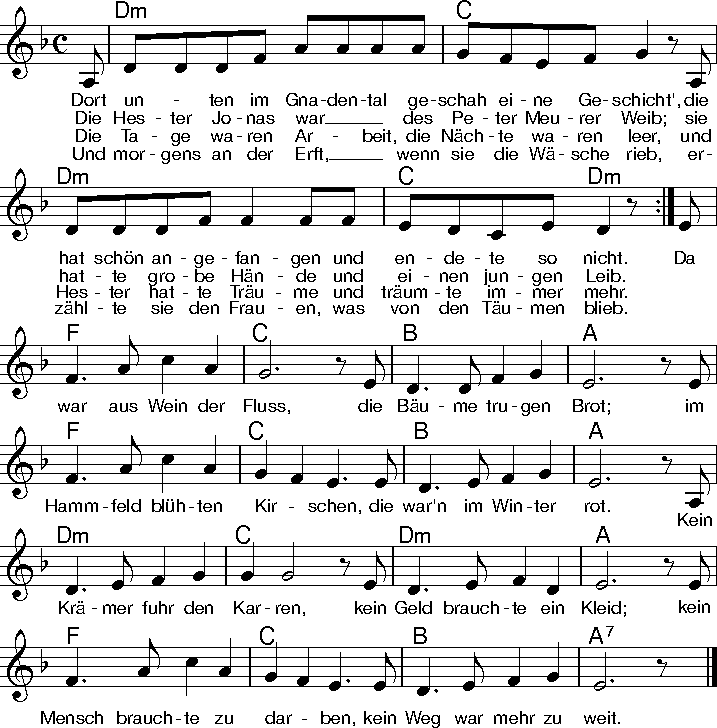
\includegraphics[draft=false, width=1\textwidth]{Noten/Lied049x.pdf}	

\beginverse
Die \[Dm]Frauen hörten sie mit \[C]lachendem Gesicht;
schön \[Dm]waren Hesters Träume und \[C]schadeten doch \[Dm]nicht. 
Und \[Dm]mittags auf dem Markt, wo \[C]mancher Händler rief,
ge\[Dm]schah's, dass um die Jonas mehr \[C]Volk zusammen\[Dm]lief. \newpage
Die \[Dm]Männer zeigten ihr oft \[C]einen schiefen Mund. 
Die \[Dm]besser'n sagten: ''Hester, du \[C]richtest dich zu\[Dm]grund'.''
Des \[Dm]Nachts zum kühlen Gras ka\[C]men sie hungrig doch  
und \[Dm]wollten Hesters Träume und \[C]baten: ''Heute \[Dm]noch.''
\endverse

\beginchorus
Die \[F]Städte werden \[C]fall'n, wo \[B]reich nur wenig \[A]sind;
die \[F]armen Leute \[C]steigen zum \[B]Reichtum ohne \[A7]Sünd'.
Und \[Dm]gibt nicht mehr \[C]den Fürst, nicht \[Dm]Bischof und den \[A]Zar 
und \[F]wird nichts sein am \[C]Morgen, wie \[B]es am Abend \[A7]war.
\endchorus

\beginverse
Da ^kamen in der Früh' zwei ^Männer aus der Stadt 
und ^schleppten Hester Jonas vor ^einen Magis^trat. 
Da ^war die Red' von Gott, da ^war die Red' von ihr,
da ^war die Red' von Träumen, die ^kränken Mensch und ^Tier.
Und ^quetschten ihr den Hals und ^brachen ihr Gebein;
die ^ganze Stadt hat Tage voll ^Hester Jonas' ^Schrei'n.
Und ^unterschrieb die Schuld mit ^der verkrümmten Hand 
und ^schrie noch lange Träume, bis ^sie das Feuer ^fand.
\endverse

\beginchorus
Die \[F]Städte werden \[C]fall'n, wo \[B]reich nur wenig \[A]sind; ...
\endchorus

\beginverse
Dort \[Dm]unten im Gnadental ge\[C]schah eine Geschicht', 
die \[Dm]hat schön angefangen und \[C]endete so \[Dm]nicht.
\endverse

\endsong

\beginscripture{}
Siehe Seite 162
\endscripture

%\beginscripture{}
%Die sogenannte Hexe von Neuss (Ort bei Düsseldorf) - geboren um 1570 - wurde wegen massiven öffentlichen Gerüchten verhaftet und verhört. Man warf der Hebamme und Kräuterheilkundlerin Schadenzauber, den Abfall von Gott und einen Pakt mit dem Teufel vor, was die Hester nach brutaler Folter auch bestätigte. Nach zwischenzeitlicher Flucht wurde sie am 24. Dezember 1935 enthauptet.
%\endscripture

\beginsong{Heute hier, morgen dort}[
    wuw={Hannes Wader}, 
    jahr={1972}, 
    bo={180}, 
    pfii={99}, 
    pfiii={29}, 
    kssiv={82}, 
    siru={99},
    tonspur={294}, 
]

\beginverse
\endverse
\includegraphics[draft=false, width=1\textwidth]{Noten/Lied050.pdf}	

\beginverse
Dass man \[C]mich kaum vermisst, schon nach \[F]Tagen ver\[C]gisst,
wenn ich längst wieder \[Am]anderswo \[G]bin,
stört und \[C]kümmert mich nicht, vielleicht \[F]bleibt mein Ge\[C]sicht
doch dem \[Am]ein' oder \[G]and'ren im \[C]Sinn.
\endverse

\beginchorus
Manchmal \[G]träume ich schwer und dann \[F]denk' ich, es \[C]wär'
Zeit zu \[G]bleiben und nun was ganz \[F]and'res zu \[C]tun.
So vergeht Jahr um Jahr und es \[F]ist mir längst \[C]klar,
dass nichts \[Am]bleibt, dass nichts \[G]bleibt, wie es \[C]war.
\endchorus

\beginverse
Fragt mich ^einer, warum ich so ^bin, bleib ich ^stumm,
denn die Antwort da^rauf fällt mir ^schwer.
Denn was ^neu ist, wird alt, und was ^gestern noch ^galt,
stimmt schon ^heut' oder ^morgen nicht ^mehr.
\endverse

\beginchorus
Manchmal \[G]träume ich schwer und dann \[F]denk' ich, es \[C]wär'
Zeit zu \[G]bleiben und nun was ganz \[F]and'res zu \[C]tun.
So vergeht Jahr um Jahr und es \[F]ist mir längst \[C]klar,
dass nichts \[Am]bleibt, dass nichts \[G]bleibt, wie es \[C]war.
\endchorus

\endsong

\beginscripture{}
Die Melodie zu ''Heute hier, morgen dort'' entstammt dem Song ''Indian Summer'' des Musikers Gary Bolstad um 1960. Hannes Wader schrieb zur Melodie, die er in einem Berliner Folkclub aufschnappte, den heute bekannten Text. Gary Bolstad übersetzte 1997 den deutschen Text von Hannes Wader wiederum ins Englische. 
Das Lied knüpft thematisch an das Gefühl in der Wandervogelbewegung an.
\endscripture

\beginsong{Hochzeit}[
    mel={Alexander Rosenbaum},
    txt={aus dem Russischen: Fotler (Erik Schellhorn), Igor Plachonin},
    txtjahr={2000}, 
    biest={538}, 
    index={Dieses kleine Winzorchester},
]

% \beginverse
% \[Dm]Dieses kleine Winzorchester, gönnt euch ruhe etwas später,
% \[Gm]also, Geiger, \[A]fröhlich soll es \[Dm]sein! \[Gm]Hej, \[A]hej!
% \[Dm]Leute macht nun Platz zum Tanzen, Musikanten, quält die Tasten,
% \[Gm]singt für eure \[A]Gäste, haut mal \[Dm]rein! \[C]
% \[F]Draußen da \[C]dunkelt’s lange \[F]schon, \[A]oh,
% \[Dm]nach Hause \[C]will noch keiner \[F]geh’n, \[C]ach!
% \[F]Ein leeres \[C]Weinfass ist der \[F]Lohn, \[A]oh,
% \[Gm]irgendeiner \[Dm]wird nach \[A]Neuem \[Dm]seh’n.
% \endverse
%
% \beginchorus
% Und jetzt kommt's: \[Dm]Hochzeit, Hochzeit, im \[C]Leben nur ein\[F]mal!
% \[Gm]Manche machen's öfter, doch \[A]ist das nicht nor\[Dm]mal.
% Und nochmal: \[Dm]Hochzeit, Hochzeit, im \[C]Leben nur ein\[F]mal!
% \[Gm]Manche machen‘s öfter, doch \[A]ist das nicht \[Dm]normal.
% \endchorus
\beginverse
\endverse
\includegraphics[draft=false, page=1]{Noten/Hochzeit.pdf}


\beginverse\memorize
\[Dm]Also Kinder, noch mehr lustig, Saiten, Finger sind schon blutig,
\[Gm]Kavaliere \[A]zieh’n die Sakkos \[Dm]aus. \[Gm]Hej, \[A]hej!
\[Dm]Nicht für Groschen, nur für Freunde tanzt der Bräutigam ne Runde,
\[Gm]schaut die Braut auf \[A]Zehenspitzen \[Dm]zu. \[C]
\endverse

\beginchorus
\[F]Lass doch den \[C]eis’gen Winter\[F]wind, \[A]oj,
\[Dm]schaukeln ein \[C]trübes Lampen\[F]licht, \[C]ach!
\[F]Schenket \[C]ein noch heut ge\[F]schwind, \[A]oj,
\[Gm]Lieder dreh’n sich \[Dm]mir im \[A]Kopf da\[Dm]nach.
Und jetzt kommt's: \[Dm]Hochzeit, Hochzeit, im \[C]Leben nur ein\[F]mal!
\[Gm]Manche machen's öfter, doch \[A]ist das nicht nor\[Dm]mal.
Und nochmal: \[Dm]Hochzeit, Hochzeit, im \[C]Leben nur ein\[F]mal!
\[Gm]Manche machen‘s öfter, doch \[A]ist das nicht \[Dm]normal.
\endchorus

\beginverse
^Heda, Mama, darf man das denn, tanzen will nunmal gelernt sein,
^doch ich bitte ^dich, tu dir nicht ^weh. ^Hej, ^hej!
^Ausgelassen spielet, Kinder, diese Welt sie zeigt mir wieder:
^Solang ich noch ^lache, lebe ^ich! ^
\endverse

\printchorus

\endsong
\beginsong{Horizont-Lied}[
    index={Ich bin viel rumgekommen},
]

\beginverse
\endverse
\includegraphics[draft=false, width=1\textwidth]{Noten/Horizont.pdf}

\beginverse
\[G]Wo ist dein zu\[C]hause, von \[D]wie weit kommst du \[G]her?
Und wie es sich so \[C]lebt bei dir, das \[Am]interessiert mich \[D]sehr.
\[G]Was ist bei dir \[C]anders? \[D]Was dir so ge\[G]fällt.
Das \[G]will ich wirklich \[F]wissen - komm \[C]zeig mir deine \[D]Welt.
Die \[C]will ich gerne \[Em]seh'n und \[G]will dich ver\[D]stehn.
\endverse

\beginchorus
\[G] Komm' \[D]los, \[C]in ein neues Land.\[G]
\[]\[]\[] Nicht al\[D]lein, wir \[C]gehen Hand in \[G]Hand.
Er\[Em]kunden wir den \[Am]Horizont, geh'n \[C]weiter als bis\[D]her.
\[G]Alles zu ent\[C]decken und \[D]morgen noch viel \[G]mehr.
\endchorus

\beginverse
Den ^Horizont als ^Zeichen, uner^reichbar und doch ^da.
Wenn ^Himmel sich und ^Erde treffen,^ist Gott für mich ^nah.
Wie ^diese dünne ^Linie, die die ^ganze Welt um^fasst,
so ^ist Gott immer ^da für mich, auch ^wenn's mir grad nicht ^passt.
Ein ^Zelt ist Gottes ^Hand - ^über mir ge\[D]spannt.
\endverse

\printchorus

\endsong

\setthumb{J}{10}
\beginsong{Jalava}[
    wuw={Schmetterlinge}, 
    alb={Proletenpassion}, 
    jahr={1976}, 
    bo={346}, 
    pfii={44}, 
    pfiii={22}, 
    siru={243}, 
    tonspur={552}, 
    index={Von Sonn' und Kessel},
]

\beginverse
Von \[Am]Sonn' und Kessel schwarz gebrannt und auch vom scharfen \[E]Wind,
steht Jalava am Führerstand, wo Dampf und Flammen \[Am]sind.
Sein \[Dm]neuer Heizer ist dabei, der \[Am]ihm das Feuer nährt,
auf der \[E]Lokomotive zwei-neun-drei, die \[Am]heut nach Russland \[E]fährt.
Ein \[Am]kleiner Mann von schmalem Bau, der werkt dort auf der \[E]Brücke,
Ruß im Gesicht, das Haar ist grau, es war eine Pe\[Am]rücke.
\endverse

\beginchorus
\[Dm]Jalava, Jalava, du Finne, was \[Am]lachst du gegen den Wind?
Ich \[E]lache, weil meine Sinne\[Am] alle beisammen sind
und \[Dm]weil wir weiterkamen und \[Am]weil der Wind sich dreht
und \[E]weil mein Heizer von Flammen und \[Am]Dampfkesseln \[E]was ver\[Am]steht.
\[Dm]Jam-pa pam-pa-di-a, \[Am]jam-pa pam-pa-di-a, \[E]jam-pa pam-pa-di, \[Am]hey, hey, \[A]hey, hey!
\[Dm]Jam-pa pam-pa-di-a, \[Am]jam-pa pam-pa-di-a, \[E]jam-pa pam-pa-di, \[Am]hey, \[E]hey, \[Am]hey!
\endchorus

\beginverse
Sie \[Am]dampften ein in Beloostrov, wo Schocks von Offi\[E]zieren
die Züge auf dem Grenzbahnhof penibel kontrol\[Am]lieren.
Sie \[Dm]prüfen jegliches Gesicht bei \[Am]ihrer Inspizierung,
doch \[E]sehen sie am Kessel nicht den \[Am]Staatsfeind der Re\[E]gierung.
\[Am]Jalava weiß, worum es geht, und langsam dampft vor\[E]bei
am letzten Posten, der da steht, Lokomotive zwei-neun-\[Am]drei.
\endverse 

\beginchorus
\[Dm]Jalava, Jalava, du Finne, was \[Am]lachst du gegen den Wind?
Ich \[E]lache, weil meine Sinne\[Am] alle beisammen sind
und \[Dm]weil wir weiterkamen und \[Am]weil der Wind sich dreht
und \[E]weil mein Heizer von Flammen und \[Am]Dampfkesseln \[E]was ver\[Am]steht.
\[Dm]Jam-pa pam-pa-di-a, \[Am]jam-pa pam-pa-di-a, \[E]jam-pa pam-pa-di, \[Am]hey, hey, \[A]hey, hey!
\[Dm]Jam-pa pam-pa-di-a, \[Am]jam-pa pam-pa-di-a, \[E]jam-pa pam-pa-di, \[Am]hey, \[E]hey, \[Am]hey!
\endchorus

\beginverse
Da ^saust die Grenzstation vorbei, die Birken stehen ^nackt,
die Lokomotive zwei-neun-drei schnauft in erhöhtem ^Takt.
Und ^Jalava lacht in den Wind, in ^den Oktoberregen:
''^Heizer, wenn wir drüben sind, dann ^wird sich was be^wegen.''
Jetzt ^schneidet der Oktoberwind die letzten Äpfel ^an,
die an den kahlen Bäumen sind an der finnischen Eisen^bahn.
\endverse

\beginchorus
\[Dm]Jalava, Jalava, du Finne, was \[Am]lachst du gegen den Wind?
Ich \[E]lache, weil meine Sinne\[Am] alle beisammen sind
und \[Dm]weil uns die Fahrt in den Bahnhof \[Am]hinter der Grenze führt
und \[E]Wladimir Iljitsch Uljanow, mein \[Am]Heizer, die \[E]Flammen \[Am]schürt.
\[Dm]Jam-pa pam-pa-di-a, \[Am]jam-pa pam-pa-di-a, \[E]jam-pa pam-pa-di, \[Am]hey, hey, \[A]hey, hey!
\[Dm]Jam-pa pam-pa-di-a, \[Am]jam-pa pam-pa-di-a, \[E]jam-pa pam-pa-di, \[Am]hey, \[E]hey, \[Am]hey!
\endchorus

\endsong

%\beginscripture{}
%Lenin (Wladimir Iljitsch Uljanow) floh im Juli 1917 nach einem missglückten Aufstand (sog. Julitage) über die russische Grenze nach Finnland. Von dort sandte er Anweisungen an seine Verbündeten in Russland und bereitete so die Oktoberevolution vor.
%Erst kurz vor Ausbruch der Revolution am 25. Oktober 1917 kehrte Lenin heimlich nach Petersburg zurück. Das Lied erzählt, wie Lenin sich, als Heizer verkleidet, mit der Lokomotive des finnischen Lokführers (und Kommunisten) Hugo Erikowitsch Jalava über die Grenze schmuggeln lässt. Die Heizer-Schmuggelei fand dabei eigentlich bei der Flucht aus Russland, nicht bei der Rückkehr nach Petersburg, statt; bei dieser verkleidete sich Lenin als finnischer lutheranischer Pastor, mit Perücke und abrasiertem Bart.
%\endscripture

\beginsong{Jerchenkow}[
    txt={deutsch von peer (Dieter Krolle)}, 
    txtjahr={1958}, 
    mel={nach einem ukrainischen Volkslied}, 
    bo={214}, 
    pfii={40}, 
    pfiii={18}, 
    siru={148}, 
    tonspur={362}, 
    index={Jeden Abend träumt Jerchenkow},
]

\beginverse
\endverse
\includegraphics[draft=false, width=1\textwidth]{Noten/Lied057.pdf}	

\beginverse*
{\nolyrics \[Dm] \[Am] \[E] \[Am] \[Dm] \[Am] \[E] \[Am-E-Am]}
\endverse

\beginverse\memorize
Als der \[Am]Mond stand nachts am Himmel, klopften \[E]wir beim Starosten \[Am]an.
Alles klauten wir dem Lümmel, selbst den \[E]roten Sara\[Am]fan.
\endverse

\beginchorus
Man \[Dm]müsste wieder \[Am]zwei Pistolen \[E]und ein Pferdchen \[Am]haben,
da\[Dm]zu mit einer \[Am]Reiterschar nach \[E]Nischnij Nowgorod \[Am]traben.
Man \[Dm]müsste wieder \[Am]zwei Pistolen \[E]und ein Pferdchen \[Am]haben,
da\[Dm]zu mit einer \[Am]Reiterschar nach \[E]Nischnij Nowgorod \[Am]tr\[E]ab\[Am]en.
\nolyrics \[Dm] \[Am] \[E] \[Am] \[Dm] \[Am] \[E] \[Am-E-Am]
\endchorus

\beginverse 
Dreimal ^ritt ich nach Odessa, dreimal ^sah ich Peters^burg
als des Zaren Leibkosaken unter ^Hebnio Sara^tow.
\endverse

\printchorus

\beginverse
An die ^vielen langen Feste denk' ich ^sehnsuchtsvoll zu^rück;
Vodkafässer, Tanzen, Singen, diese ^Zeit kehrt nie zu^rück.
\endverse

\printchorus

\endsong

\beginscripture{}
Nischnij (auch: Nischni) Nowgorod = fünftgrößte russische Stadt, Industrie-Metropole; Starost = Vermögen Verwaltender (etwa: Vorsteher);
Die wahren Identitäten Jerchenkows sowie Hebnio Saratows, insofern es sie gibt, sind unbekannt.
\endscripture

\setthumb{K}{11}
\beginsong{Kaspar}[
    wuw={Reinhard Mey}, 
    jahr={1968}, 
    pfii={94}, 
    pfiii={45}, 
    gruen={18}, 
    kssiv={68}, 
    siru={212}, 
    tonspur={462}, 
    index={Sie sagten, er käme von Nürnberg her},
]

\beginverse\memorize
Sie \[Am]sagten, er käme von \[D]Nürnberg her und er \[Am]spräche kein Wort. Auf dem Marktplatz standen sie \[D]um ihn her und be\[Am]gafften ihn dort. Die \[C]einen raunten: ''Er ist ein Tier'',\[Am] die ander'n fragten: ''Was will der hier?''\[D] und dass er sich doch zum \[G]Teufel scher  ''So \[C]jagt ihn doch fort,\[E7] so \[Am]jagt ihn doch fort!''
\endverse


\beginverse\memorize
Sein \[Am]Haar in Strähnen und \[D]wirre, sein \[Am]Gang war gebeugt. ''Seht, dieser arme \[D]Irre ward vom \[Am]Teufel gezeugt.'' Der \[C]Pfarrer reichte ihm einen Krug voll \[Am]Milch, er trank in einem Zug.\[D] ''Der trinkt nicht vom Ge\[G]schirre, den hat die \[C]Wölfin gesäugt,\[E7]  den hat die \[Am]Wölfin gesäugt.''
\endverse

\beginverse
Mein ^Vater, der in ^unserem Orte ^Schulmeister war, trat zu ihm hin, trotz ^böser Worte ^rings aus der Schar. Er ^sprach zu ihm ganz ruhig und der ^Stumme öffnete den Mund und ^stammelte die ^Worte ''Heiße ^Kaspar,^ heiße ^Kaspar.''
\endverse 

\beginverse
Mein ^Vater brachte ihn ^mit nach Haus, ''Heiße ^Kaspar.'' Meine Mutter wusch seine ^Kleider aus und ^schnitt ihm das Haar. ^ Sprechen lehrte mein Vater ihn,^ lesen und schreiben und es schien, was man ihn ^lehrte, sog er in sich ^auf, wie ^gierig er war,^ wie ^gierig er war.
\endverse

\beginverse
Zur ^Schule gehörte der^zeit noch das ^Üttinger Feld. Kaspar und ich, wir ^pflügten zu zweit, bald war ^alles bestellt. Wir ^hegten und pflegten jeden Keim,^ brachten im Herbst die Ernte ein, von den ^Leuten vermale^deit, von ihren ^Hunden verbellt,^ von ihren ^Hunden verbellt.
\endverse

\beginverse
Ein ^Wintertag, der ^Schnee lag frisch, es war ^Januar. Meine Mutter rief uns: ''^Kommt zu Tisch, das ^Essen ist gar.'' Mein ^Vater sagte: ''Appetit'',^ ich wartete auf Kaspars Schritt, mein ^Vater fragte ^mürrisch: ''Wo bleibt ^Kaspar,^ wo bleibt ^Kaspar?''
\endverse

\beginverse
Wir ^suchten und wir ^fanden ihn auf dem ^Pfad bei dem Feld. Der Neuschnee wehte ^über ihn, sein Ge^sicht war entstellt, die ^Augen angstvoll aufgerissen,^ sein Hemd war blutig und zerrissen.^ Erstochen hatten sie ^ihn dort am ^Üttinger Feld,^ dort am ^Üttinger Feld.
\endverse

\beginverse
Der ^Polizeirat aus der ^Stadt füllte ^ein Formular. ''Gott nehm' ihn hin in ^seiner Gnad'', sagte ^der Herr Vikar. Das ^Üttinger Feld liegt lang schon brach,^ nur manchmal bell'n mir noch die Hunde nach,^ dann streu' ich ein paar Blumen auf ^den Pfad für ^Kaspar,^ für ^Kaspar.
\endverse

\endsong

\beginscripture{}
Kaspar Hauser tauchte am 26. Mai 1828 plötzlich in Nürnberg auf. Er war verwahrlost, sprach kaum, konnte nur schlecht gehen und behauptete, sein Leben in Dunkelheit in einer Zelle verbracht zu haben. Er führte einen anonymen Brief mit sich, welcher Nahe legte, er sei seit seiner Kindheit isoliert gewesen.
Hauser wurde betreut und lernte schnell, blieb aber psychisch labil. Über seine Herkunft gab es viele Spekulationen – etwa, er sei ein badischer Erbprinz.
Am 14. Dezember 1833 wurde er mit einer Stichwunde aufgefunden und starb drei Tage später. Ob er ermordet wurde oder sich selbst verletzte, ist bis heute unklar. \\

Auf seinem Grabstein steht~ ''Hier liegt Kaspar Hauser, Rätsel seiner Zeit, unbekannt die Herkunft, geheimnisvoll der Tod 1833.''
\endscripture


\setthumb{L}{12}
\beginsong{Leise weht der Wind}[
    wuw={von einer Großfahrt des BdP ins Belledonne-Massiv}, 
    jahr={1983}, 
    bo={228}, 
    pfii={92}, 
    pfiii={28}, 
    gruen={30}, 
    kssiv={8}, 
    siru={157},
    tonspur={379}, 
]

\beginverse
\[Am] Leise weht der Wind über grünen \[Em]Bäumen,
der Berg grüßt uns von \[F]fern, wir möchten alle \[G]gern mit ihm \[Am]träumen.
Leise weht der Wind über grünen \[Em]Bäumen,
vor uns liegt der \[F]Pfad, er führt auf den \[G]Grat, von wo die Wasser \[Am]schäumen.
\endverse

\beginchorus
Vor uns läuft ein \[G]Schweigen auf dem Weg da\[Am]von
und man gab ihm einen \[G]Namen: Man nannte es Belle\[Am]donne.
Der Berg ist wie ein \[G]König, die Krone ganz aus \[Am]Eis,
eine Schleppe voller \[G]Blumen, jung und doch ein \[Am]Greis.
\endchorus

\beginverse
^ Leise weht der Wind über kahlen ^Steinen,
ein letzter Blick zu^rück, dort liegt nicht das ^Glück, das wir ^meinen.
Leise weht der Wind über kahlen ^Steinen,
nur wer den Berg ver^steht, auf den Gipfel ^geht, denn Grenzen gibt es ^keine.
\endverse

\printchorus

\beginverse
^ Leise weht der Wind über Gletscher^seen.
Wie weit werden wir noch ^kommen? Die Kraft ist uns ge^nommen,
doch die Fahrt wird weiter^gehen.
Leise weht der Wind über Gletscher^seen.
Unser Ziel erreicht, wir ^scherzen, vergessen alle ^Schmerzen,
wenn wir über allem ^stehen.
\endverse

\beginchorus
Vor uns läuft ein \[G]Schweigen auf dem Weg da\[Am]von
und man gab ihm einen \[G]Namen: Man nannte es Belle\[Am]donne.
Der Berg ist wie ein \[G]König, die Krone ganz aus \[Am]Eis,
eine Schleppe voller \[G]Blumen, jung und doch ein \[Am]Greis.
\endchorus

\beginverse
^ Leise weht der Wind über's Alltags^leben,
vor uns liegt die ^Stadt, die keine Seele ^hat.
Was ist der Berg da^gegen?
Leise weht der Wind über's Alltags^leben,
ab und zu dreh'n wir uns ^um, doch die Gipfel bleiben ^stumm,
wir möchten gern' mit ihnen ^reden.
\endverse

\beginchorus
Vor uns liegt die \[G]Eile der Zivilisa\[Am]tion,
doch wir kehren \[G]wieder zu uns'rem Freund Belle\[Am]donne.
Er ist wie ein \[G]König, die Krone ganz aus \[Am]Eis,
eine Schleppe voller \[G]Blumen und der Wind weht \[Am]leis'.
\endchorus

\endsong

\beginscripture{}
Das Belledonne-Massiv ist ein 60 km langer Ausläufer der Alpen in Ostfrankreich, das bis in 2.980m Höhe reicht.
\endscripture


\setthumb{M}{13}
\beginsong{Marktfrauen, Kinder und Troubadoure}[
    wuw={rumpel (Andreas Barth), BdP Löwenherz, Marburg}, 
    jahr={1992}, 
    bo={270}, 
    pfii={39}, 
    pfiii={49}, 
    siru={202}, 
    tonspur={444}, 
    index={Scharlatane, eins will ich euch},
]

\beginverse
\endverse
\includegraphics[draft=false, width=1\textwidth]{Noten/Lied063.pdf}	

\beginverse
\[Em]Sie war’n nicht \[D]lange im \[C]Ne\[D]bel ver\[Em]borgen,
sie hat nicht \[D]lange die \[C]Blind\[D]heit ge\[Em]quält.
\[Em]Sie haben \[D]Einfall um \[C]Ein\[D]fall ge\[Em]boren,
haben \[D]Gefahr und \[C]Frei\[D]heit ge\[Em]wählt.
\lrep Sie sind nicht \[D]feige, \[F]ängstlich und \[Am]klein.
\[Em]Marktfrauen, \[D]Kinder und \[C]Trou\[D]ba\[Em]doure
\[Em]tanzen in \[D]unsere \[C]Zeit \[D]hi\[Em]nein. \rrep
\endverse

\beginverse
^Trotzen der ^Macht, die mit ^Angst ^Menschen ^presste,
die allen ^Mut zu ^fra^gen ver^bannt.
^Feiern in^mitten der ^Ker^ker die ^Feste,
bauen ihr ^Zelt auf ver^bo^tenes ^Land.
\lrep Blumen er^blüh'n im ^grauen Ge^stein.
^Marktfrauen, ^Kinder und ^Trou^ba^doure,
^bunter ^Tanz in die ^Welt ^hi^nein. \rrep
\endverse

\endsong

\input{Lieder/Miruschka}
\beginsong{Molly Malone}[
    wuw={James Yorkston}, 
    jahr={1883}, 
    bo={210}, 
    pfii={205}, 
    kssiv={134}, 
    biest={579}, 
    siru={134}, 
    index={In Dublin's fair city},
]

\beginverse
\endverse
\includegraphics[draft=false, width=1\textwidth]{Noten/Lied066.pdf}

\beginverse
She \[C]was a fish\[Am]monger, which \[Dm]was no \[G7]wonder
for \[C]so was her \[Am]father and \[Dm]mother be\[G7]fore.
And they \[C]both wheeled their bar\[Am]row
through \[Dm]streets broad and \[G7]narrow, crying:
\[C]Cockles and \[Am]mussels, a\[C]live, a\[G7]live, \[C]oh!
A\[C]live, alive, \[Am]oh, a\[Dm]live, alive, \[G7]oh! Crying:
\[C]Cockles and \[Am]mussels, a\[C]live, a\[G7]live, \[C]oh!
\endverse

\beginverse
She ^died of a ^fever and ^no one could ^save her
and ^that was the ^end of sweet ^Molly Ma^lone.
But her ^ghost wheels her ^barrow
through ^streets broad and ^narrow, crying:
^Cockles and ^mussels, a^live, a^live, ^oh!
A^live, alive, ^oh, a^live, alive, ^oh! Crying:
^Cockles and ^mussels, a^live, a^live, ^oh!
\endverse

\endsong

\beginscripture{}
Molly Malone, auch bekannt unter dem Titel~ ''Cockles and Mussels'' (Herzmuscheln und Miesmuscheln), ist ein bekanntes irisches Volkslied und eine inoffizielle Hymne der Stadt Dublin. Die Ballade erzählt die Geschichte einer schönen Dubliner Fischhändlerin, die in jungen Jahren an nicht näher bestimmtem Fieber stirbt.
Das Lied wurde auch in der Stanley-Kubrick-Verfilmung von~ ''A Clockwork Orange'' verwendet: In einer der Schlüsselszenen singt ein betrunkener Landstreicher das Lied.
\endscripture



\setthumb{N}{14}
\beginsong{Nacht in Portugal}[
    wuw={Dimitrie Miron (Deutscher Pfadfinderbund Mosaik, Stamm Sperber)}, 
    siru={268}, 
    biest={647}, 
    buedel={359},
    index={Wenn die Sonne sich schon},
]

\beginverse
\endverse
\includegraphics[draft=false, page=1]{Noten/NachtInPortugal.pdf}

% \beginverse\memorize
% Wenn die Sonne sich schon \[Am]senkt, geschieht es ein ums and're \[G]Mal,
% werden Lampen aufge\[F]hängt in dem Dorf in Portu\[E]gal.
% Und wie schon in alter \[Am]Zeit kommt ein Jeder ohne \[G]Hatz,
% die Gitarren sind \[F]bereit, schon erfüllt Musik den \[E]Platz.
% \endverse
%
% \beginchorus
% \lrep Und sie beginnen zu \[Am]tanzen, das Dorf bewegt sich im \[G]Ganzen,
% selbst Kinder und \[F]Greise auf eigene Weise, sie drehn sich im \[E]Kreise. \rrep
% \endchorus

\beginverse
In dieser warmen Juli\[Am]nacht zeigen sie ihr Temp'ra\[G]ment,
keine Pause wird ge\[F]macht und sie tanzen wie ent\[E]hemmt.
Sieht ein Fremder dieses \[Am]Bild, bleibt er nicht sehr lang \[G]allein,
bald tanzt er genauso \[F]wild und es wirbeln seine \[E]Bein'.
\endverse

\renewcommand{\everychorus}{\textnote{\bf Refrain 2}}
\beginchorus
\lrep Und so tanzen sie \[Am]immer, bis der erste Sonnen\[G]schimmer,
die Strahlen aus\[F]sendet, die Augen schon blendet und den Tanz be\[E]endet. \rrep 
\endchorus

\renewcommand{\everychorus}{\textnote{\bf Refrain 1 und Zwischenspiel}}
\beginchorus
\lrep Und sie beginnen zu \[Am]tanzen, das Dorf bewegt sich im \[G]Ganzen,
selbst Kinder und \[F]Greise auf eigene Weise, sie drehn sich im \[E]Kreise. \rrep
\endchorus

\endsong

\beginsong{Nachts auf dem Dorfplatz}[
    wuw={turi (Kurt Kremers)}, 
    jahr={1964}, 
    bo={240},
    pfii={116}, 
    gruen={57}, 
    kssiv={24}, 
    siru={167}, 
    tonspur={406},
]

\beginverse
\endverse
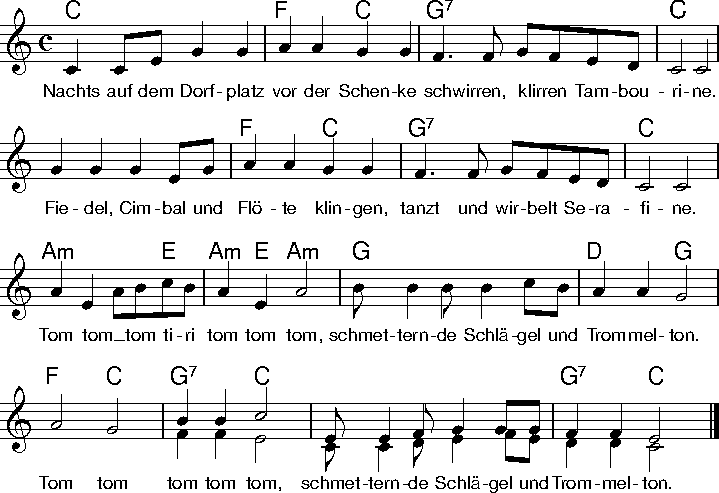
\includegraphics[draft=false, width=1\textwidth]{Noten/Lied067.pdf}

\beginverse
\[C]Her mit dem Weinkrug \[F]voll zum \[C]Rande, \[G7]trinkt zur Neige, durst'ge \[C]Zecher!
Zigan, spielst du die \[F]Sara\[C]bande, \[G]lockt als Lohn ein gold'ner \[C]Becher.
\endverse

\beginchorus
\[Am]Tom tom tom \[E]tiri \[Am]tom \[E]tom \[Am]tom, \[G]schmetternde Schlägel und \[D]Trommel\[G]ton:
\[F]Tom \[C]tom \[G7]tom tom \[C]tom, schmetternde Schlägel und \[G7]Trommel\[C]ton.
\endchorus
 
\beginverse
^Knöcherne Finger ^alter ^Fetteln ^lesen Zukunft aus den ^Händen,
Pfeife rauchend und ^Tabak ^bettelnd, ^dürre Beine, feiste ^Lenden.
\endverse

\beginchorus
\[Am]Tom tom tom \[E]tiri \[Am]tom \[E]tom \[Am]tom, \[G]schmetternde Schlägel und \[D]Trommel\[G]ton:
\[F]Tom \[C]tom \[G7]tom tom \[C]tom, schmetternde Schlägel und \[G7]Trommel\[C]ton.
\endchorus

\beginverse
^Segelt des Mondes ^stille ^Barke ^über Pinien und Pla^tanen.
Mitternacht wird zur ^Wende^marke, ^lässt den jungen Tag schon ^ahnen.
\endverse

\beginchorus
\[Am]Tom tom tom \[E]tiri \[Am]tom \[E]tom \[Am]tom, \[G]leis' werden Schlägel und \[D]Trommel\[G]ton:
\lrep \[F]Tom \[C]tom \[G7]tom tom \[C]tom, leis' werden Schlägel und \[G7]Trommel\[C]ton. \rrep
\endchorus

\endsong

\beginscripture{}
Das Lied ist auch bekannt unter dem Titel~ ''Die Schenke von Novo Selo''.
\endscripture

\beginsong{Nehmt Abschied, Brüder}[
    wuw={Robert Burns (aus dem Schottischen)}, 
    txt={Claus Ludwig Laue (Übersetzung)}, 
    txtjahr={zwischen 1759 und 1796}, 
    bo={246}, 
    pfii={2}, 
    pfiii={3}, 
    kssiv={51}, 
    siru={169},
    tonspur={415}, 
]

\beginverse
\endverse
\includegraphics[draft=false, width=1\textwidth]{Noten/NehmtAbschiedBruederV.pdf}

\beginverse
Die \[C]Sonne sinkt, es \[G]steigt die Nacht, ver\[C]gangen ist der \[F]Tag.
Die \[C]Welt schläft ein und \[G]leis' erwacht der \[F]Nachti\[G]gallen \[C]Schlag.
\endverse

\beginchorus
Der \[C]Himmel wölbt sich \[G]über's Land. A\[C]de, auf Wieder\[F]seh'n!
Wir \[C]ruhen all in \[G]Gottes Hand. Lebt \[F]wohl, auf \[G]Wieder\[C]seh'n!
\endchorus

\beginverse
So ^ist in jedem ^Anbeginn das ^Ende nicht mehr ^weit.
Wir ^kommen her und ^gehen hin und ^mit uns ^geht die ^Zeit.
\endverse

\newpage

\beginchorus
Der \[C]Himmel wölbt sich \[G]über's Land. A\[C]de, auf Wieder\[F]seh'n!
Wir \[C]ruhen all in \[G]Gottes Hand. Lebt \[F]wohl, auf \[G]Wieder\[C]seh'n!
\endchorus

\beginverse
Nehmt ^Abschied Brüder, ^schließt den Kreis; das ^Leben ist ein ^Spiel.
Nur ^wer es recht zu ^leben weiß, ge^langt ans ^große ^Ziel.
\endverse

\beginchorus
Der \[C]Himmel wölbt sich \[G]über's Land. A\[C]de, auf Wieder\[F]seh'n!
Wir \[C]ruhen all in \[G]Gottes Hand. Lebt \[F]wohl, auf \[G]Wieder\[C]seh'n!
\endchorus

\endsong

\beginscripture{}
Auld Lang Syne ist der Titel eines der bekanntesten Lieder im englischsprachigen Raum. Sinngemäß bedeutet der Titel soviel wie~ ''längst vergangene Zeit''. Es wird in der anglophonen Welt traditionsgemäß zum Jahreswechsel gesungen, um der Verstorbenen des zu Ende gegangenen Jahres zu gedenken. Der deutsche Titel lautet~ ''Nehmt Abschied, Brüder''. In der Pfadfinderbewegung gilt es weltweit als Abschiedslied, das am Ende von Veranstaltungen gesungen wird.

Wegen der Verwendung in der Pfadfinderbewegung wurde das Lied in zahlreiche Sprachen übertragen. Die deutsche Übertragung~ ''Nehmt Abschied, Brüder'' von Claus Ludwig Laue entstand für die Deutsche Pfadfinderschaft Sankt Georg.
\endscripture

\beginsong{Nordwärts}[
    wuw={Silke Neumann}, 
    jahr={1982},
    bo={248}, 
    pfii={60}, 
    pfiii={46}, 
    gruen={77}, 
    kssiv={30}, 
    siru={173}, 
    tonspur={422}, 
]

\beginverse
\endverse
\includegraphics[draft=false, width=1\textwidth]{Noten/Lied072.pdf}	

\beginverse
\[Am]Wollen frei so \[G]wie ein Vogel \[Dm]wiegen uns im \[Am]kalten Wind,
\[C]woll'n den Ruf der \[G]Wildnis hören, \[Am]wenn wir \[Dm]glück\[Em]lich \[Am]sind.
\endverse

\beginverse
^Woll'n durch Moor und ^Sümpfe waten, ^abends legen ^uns zur Ruh'.
^Klampfen sollen ^leis' erklingen, ^singen ^im^mer^zu.
\endverse

\beginverse
^In der Kohte ^brennt ein Feuer, ^füllt uns alle ^mit Bedacht.
^Schlaf senkt sich auf ^uns're Lider, ^doch die ^Wild^nis ^wacht.
\endverse

\beginverse
^Käuzchen schreien, ^Bäume rauschen ^bis zum frühen ^Morgengrau'n.
^Über ausge^qualmtem Feuern ^strahlt der ^Him^mel ^blau.
\endverse

\beginverse
^Wenn wir wieder ^heimwärts ziehen, ^sehnet jeder ^sich zurück,
^denkt an die ver^gang'nen Fahrten, ^an ver^gang'^nes ^Glück.
\endverse

\beginverse
^Nordwärts, nordwärts ^woll'n wir wieder ^zu den Bergen ^und den Seen,
^dieses Land noch^mal erleben ^und auf ^Fahr^ten ^geh'n.
\endverse

\endsong

\begin{intersong}
    \flushbottom\newpage\flushbottom
\end{intersong}

\setthumb{O}{15}

\setthumb{P}{16}
\beginsong{Piratenlied}[
    wuw={jusch (Julian Colins), BdP Berlin}, 
    jahr={2007}, 
    siru={154}, 
    biest={588},
    buedel={188}, 
    index={Klingt ein Lied durch die Nacht}, 
]

\beginverse
\endverse
\includegraphics[draft=false, page=1]{Noten/Piratenlied.pdf}	

\beginverse\memorize
Manches \[Em]Heck hat der \[D]Sturm in den \[G]Kurs uns ge\[D]lenkt, 
Und Queen \[Em]Mary die \[D]machten gleich \[C]dreimal \[D]wir \[Em]froh. \newpage
Selbst der \[Em]stolzen Fre\[D]gatte, die mit \[G]Blei uns bes\[H7]chenkt. 
Winkt der \[Am]Stückpforten Flug, unser Stolz vorn am \[Em]Bug. 
Hat \[D]noch \[G]jede \[D]ver\[G]senkt -- Pi\[H7]raten Johoo.
\endverse

\beginchorus
\lrep \[Em]Jo\[C]hoo, \[G]grüßet uns \[D]froh, \[Am]jo\[Em]hoo, \[D]fern Fala\[Em]do! \rrep
% \newline
\endchorus
%
% \includegraphics[draft=false, width=1\textwidth]{Noten/Piratenlied_1a2.pdf}
% \newpage
%
% \includegraphics[draft=false, width=1\textwidth]{Noten/Piratenlied_1b2.pdf}

\beginverse*
\bf Bridge \sf
\[(Em)]Auf Krämer\[C]seelen, Ban\[D]kiers und Kriegs\[A]helden.
Zum \[Em]höfischen \[C]Tanz -- wer nicht \[D]schwarz trägt ist \[A]bunt.
Ein \[Em]freies Ge\[C]sicht lacht im \[G]Rhythmus der \[D]Messer.
Riecht nach \[F]brennenden Planken, Schweiß, Meersalz, Fisch und mit \[G]Ahoi, einem Kuss, einem Fluch und mit Glück geht es \[H7]dreimal zum Teufel und dreimal zurück.
\endverse

\beginchorus
\lrep \[Em]Jo\[C]hoo, \[G]grüßet uns \[D]froh, \[Am]jo\[Em]hoo, \[D]fern Fala\[Em]do! \rrep
\endchorus

\beginverse
Brüder ^trinkt auf die ^See, die uns ^ruft weit hi^naus, 
Aller ^Sünder Weg ^treiben wir ^ins nir^gend^wo, 
Kehrt doch ^keiner von ^unseren ^Fahrten nach ^Haus. 
Und so ^trinkt auf dies Leben, das bleibt unver^geben!
Und ^zum ^Ende ^trinkt ^aus -- Pi^raten Johoo!
\endverse

\beginchorus
\lrep \[Em]Jo\[C]hoo, \[G]grüßet uns \[D]froh, \[Am]jo\[Em]hoo, \[D]fern Fala\[Em]do! \rrep
Und \[D]zum \[G]Ende \[D]trinkt \[G]aus -- Pi\[H7]raten Jo\[Em]hoo!
\endchorus

\endsong

% \beginscripture{}
% Uraufführung auf dem Sängerfest Burg Rabenstein.
% \endscripture


\setthumb{R}{18}
\beginsong{Raubritter}[
    wuw={nathan (Georg Hausmann) und anti (Volker Hausmann), Nerother Wandervogel}, 
    jahr={1967}, 
    bo={344}, 
    pfii={16}, 
    pfiii={6}, 
    gruen={153}, 
    kssiv={33}, 
    siru={241}, 
    tonspur={550}, 
    index={Von der Festung dröhnt},
]

\beginverse
\endverse
\includegraphics[draft=false, width=1\textwidth]{Noten/Lied077.pdf}	 

\beginverse
In \[Am]uns'rer Knechtschaft \[F]Zeit griffen wir zu \[Am]Waffen,
schlugen uns're \[F]Herr'n, Grafen und auch \[Am]Pfaffen.
\endverse

\beginchorus
\[G]Be\[C]herrschen dies Ge\[G]biet, \[Am]singen stolz ihr \[E]Lied: 
\[Am]Raubritter, Raubritter, wie weit \[G]ist \[C]un\[G]ser \[Am]Land?
\[F]Raubritter, Raubritter, wie stark \[C]ist \[F]uns'\[G]re \[Am]Hand?
\endchorus
 
\beginverse
^Groß ist uns're ^Macht, solange wir ^vereint.
Hüten uns're ^Burg, trotzen jedem ^Feind.
\endverse

\beginchorus
\[G]Be\[C]herrschen dies Ge\[G]biet, \[Am]singen stolz ihr \[E]Lied:
\[Am]Raubritter, Raubritter, wie weit \[G]ist \[C]un\[G]ser \[Am]Land?
\[F]Raubritter, Raubritter, wie stark \[C]ist \[F]uns'\[G]re \[Am]Hand?
\endchorus

\endsong

\beginscripture{}
Im Jahre 1967 spaltete sich der Orden der Raubritter vom Orden der Rabenklaue im Nerother Wandervogel ab. Das Lied wurde das Ordenslied des neu gegründeten Ordens. Es existieren viele Textvariationen, die vermutlich durch die mündliche Übetragung entstanden sind.

Als Raubritter bezeichnet man diejenigen Angehörigen des ritterlichen Standes, die sich durch Straßenraub, Fehden und Plünderungszüge bereicherten.
\endscripture

\beginsong{Regenbogenlied}[
    index={Von überall sind wir gekommen},
]

\beginverse
\endverse
\includegraphics[draft=false, width=1\textwidth]{Noten/Regenbogenlied.pdf}

\beginverse\memorize
\[C] Von Süden, Osten, \[F]West und Norden,
\[G] sind wir vereint zum \[C]großen Spiel,
\[Am] denn weit ist unser \[Dm]Kreis geworden
\[G] und nur in ihm liegt \[C]unser Ziel.
\endverse

\beginchorus
\[F] Über uns ein \[G]Regenbogen,
\[C] zeigt uns den Weg in \[Am]seinem Licht.
\[F] Die Wolken sind schon \[G]fortgezogen,
\[C] verwehren \[Dm]uns die \[G7]Sonne \[C]nicht.
\endchorus

\beginverse
^ Und abends in der ^Lagerrunde,
^ erzählen wir von ^dir und mir,
^ scheint auch kein Licht in ^dieser Stunde,
^ am nächsten Morgen ^wissen wir:
\endverse

\beginchorus
\[F] Sind wir einmal \[G]fortgezogen,
\[C] dorthin, wo es \[Am]uns gefällt,
\[F] bringt auch unser \[G]Regenbogen
\[C] neue \[Dm]Farben \[G7]in die \[C]Welt.
\endchorus

\endsong

\begin{intersong}
\flushbottom\newpage\flushbottom
\end{intersong}
\beginsong{Roter Mond}[
    wuw={Anja Klenk (Hortenring Ernsthofen)}, 
    jahr={1980}, 
    bo={266}, 
    pfii={90}, 
    pfiii={27}, 
    gruen={68}, 
    kssiv={38}, 
    siru={194},
    tonspur={436}, 
]

\transpose{-7}

\beginverse
\endverse
\includegraphics[draft=false, width=1\textwidth]{Noten/Lied078.pdf}	

\beginverse
\[Em]Sterne ste\[D]h'n hell am Firmament, \[Em]solche Nac\[D]ht findet nie ein End'.
\lrep \[G]Dieses La\[D]nd, wild und schön, und \[Am]wir dürfen seine \[Em]Herrlichkeit seh'n. \rrep
\endverse

\beginverse
^Rauher Fe^ls, Moos und Heidekraut, ^weit entfer^nt schon der Morgen graut.
\lrep ^Fahne we^ht, weiß und blau, das ^Gras schimmert unterm ^Morgentau. \rrep
\endverse

\beginverse
\[Em]Fahrt vorb\[D]ei, morgen geht es fort, \[Em]kommen w\[D]ir wieder an den Ort?
\[G]Norden i\[D]st unser Glück und \[Am]in uns bleibt nur die Er\[Em]innerung zurück.
\[G]Norden i\[D]st unser Glück und \[Am]wir schwören auf ein \[Em]neues zurück.
\endverse

\endsong

\beginscripture{}
Dieses Lied ist 1980 bei einem Pfadfinderlager des Hortenring Ernsthofen in Schweden entstanden. Die Farben "weiß und blau" beziehen sich auf das Banner des Pfadfinderbundes. Dieser Bund wurde Ende der Neunziger Jahre aufgelöst.
Wenn der Mond nah am Horizont steht, dann wird das Licht so durch die Atmosphäre gefiltert, dass er rot erscheint.
\endscripture 

\beginsong{Roter Wein im Becher}[
    wuw={Helmut König, Musik nach einem französischen Volkslied}, 
    bo={268}, 
    pfii={15}, 
    pfiii={9}, 
    gruen={76}, 
    kssiv={25}, 
    siru={195},
    tonspur={438}, 
]

\beginverse
\endverse
\includegraphics[draft=false, width=1\textwidth]{Noten/Lied079.pdf}	

\beginverse
\[Em]Morgens bricht die Runde zu \[D7]neuen Fahrten \[G]auf.
Es \[D7]klingt in aller \[G]Mun\[Am]de ein \[Em]frohes \[H7]Liedchen \[Em]auf. 
\endverse

\beginchorus
\lrep Radi, radi, ra-di \[C]rala\[G]la, \[D7]radi, radi, \[Em]ra-di \[H7]ralalala\[Em]la. \rrep
\endchorus

\beginverse
^Steine, Staub und Dornen sind ^schwerlich Tippe^lei.
Wir ^müssen uns an^spor^nen, die ^Qual ist ^bald vor^bei.
\endverse

\printchorus

\beginverse
^Treffen wir uns wieder, der ^Zufall nennt den ^Ort,
so ^schallen uns're ^Lie^der in ^weite ^Ferne ^fort.
\endverse

\printchorus

\endsong

\beginscripture{}
Tippelei = Walz, Gesellenwanderung
\endscripture


\setthumb{S}{19}
\beginsong{Die Sandbank}[
    wuw={Alexander Gorodninski},
    txt={Fotler (Erik Schellhorn), Igor Plachonin, Deutscher Fahrtenbund Zugvogel},
    txtjahr={2003},
    jahr={1960}, 
    siru={7},
    buedel={10}, 
    index={All' diese Wellen},
]

% \beginverse
% All' diese \[A7]Wellen, ja diese \[Dm]Wellen, die sollen \[C]bloß zur Hölle \[F]fahr'n, \[D7]
% \lrep\ Und keine \[Gm]Karten von diesen S\[Dm]tellen,
% Ich treibe \[Gm]vorwärts \[A7]ohne \[Dm]Plan. \rrep
% \endverse

\beginverse
\endverse
\includegraphics[draft=false, page=1]{Noten/Sandbank.pdf}

\beginverse
Irgendwo \[A7]leben die tollen \[Dm]Weiber, 
sitzt mancher \[C]Freund beim Wodka\[F]glas, \[D7]
\lrep Doch hier be\[Gm]herrschen der Wind, die \[Dm]Steine 
Mein Boot voll \[Gm]Löcher, \[A7]Moos und \[Dm]Gras. \[(D7)] \rrep
\endverse

\beginverse
Am großen ^Fluss bin ich am ^Morgen, 
der Sommer ^ist dann längst vor^bei, ^
\lrep um mich, da ^macht euch mal keine ^Sorgen, 
denn bald schon ^wieder ^ist es ^Mai.^ \rrep
\endverse

\beginverse
Aber viel^leicht gibt es dich und ^solang 
du mich nicht ^quälst mit deinem ^Leid, ^
\lrep Ich liebe ^dich, doch nur bis zur ^Sandbank, 
Was dann kommt, ^bringt uns ^schon die ^Zeit.^ \rrep
\endverse

\beginverse
All' diese ^Wellen, ja diese ^Wellen, 
die sollen ^bloß zur Hölle ^fahr'n, ^
\lrep und keine ^Karten von diesen ^Stellen, 
Ich treibe ^vorwärts ^ohne ^Plan.^ \rrep
\endverse

\endsong

\beginsong{Das Schiff im Nebel}[
    wuw={manu (Manuel Hornauer), BdP, Stamm Normannen}, 
    jahr={2012}, 
    biest={624},
    buedel={267},
    index={Siebzehn Tage fährt das Schiff},
]

% \beginverse
% \[H7]Siebzehn Tage \[Em]fährt das Schiff, durch \[Am]Nebel, Wellen, \[H7]Gischt,
% und wir \[C]haben keinen \[H7]Kurs und \[Am]auch zu \[H7]essen \[Em]nicht.
% Wir \[F]tasten uns \[C]vor, \[Am]durch die graue \[H7]Wand,
% fast \[F]stirbt in uns \[Em]schon die \[C]Hoffnung auf \[H7]Land.
% \endverse

\beginverse
\endverse
\includegraphics[draft=false, page=1]{Noten/SchiffImNebel.pdf}


\beginverse
\[H7]Ein Schlag links und \[Em]einer rechts, doch \[Am]geradeaus geht’s \[H7]nicht.
\[C]Wabernd graue \[H7]Teufelsflossen \[Am]nehmen \[H7]jedes \[Em]Licht.
\[F]Angst greift um \[C]sich, wann \[Am]endet diese \[H7]Fahrt?
Viel\[F]leicht stirbt schon \[Em]morgen \[C]auch der erste \[H7]Maat.
\endverse

\beginchorus
Wir fahr'n da\[Em]hin, wir fahr'n da\[Am]hin,
wir fahr'n da\[Em]hin, auf hoher \[H7]See.
Wir fahr'n da\[Em]hin, durch graue \[C]Not,
wir fahr'n da\[Em]hin, denn unser \[H7]Steuermann ist \[Em]tot.
\endchorus

\beginverse
Das ^Schiff im Nebel ^ist verlor’n, denn ^keiner weiß wo^hin.
Nur ^Rudern, Rudern, ^Ausschau halten ^ohne ^viel Ge^winn!
Wir ^tasten uns ^vor, ^durch die graue ^Wand,
fast ^stirbt in uns ^schon die ^Hoffnung auf ^Land.
\endverse

\beginchorus
Wir fahr'n da\[Em]hin, wir fahr'n da\[Am]hin,
wir fahr'n da\[Em]hin, auf hoher \[H7]See.
Wir fahr'n da\[Em]hin, durch graue \[C]Not,
wir fahr'n da\[Em]hin, denn unser \[H7]Steuermann ist \[Em]tot.
\endchorus

\endsong
\beginsong{Schilf}[
    wuw={tejo (Walter Scherf), Musik aus Schweden}, 
    pfii={61}, 
    pfiii={48}, 
    bo={272}, 
    kssiv={37}, 
    siru={203}, 
    tonspur={446},
]

\beginverse
\endverse
\includegraphics[draft=false, width=1\textwidth]{Noten/Lied080.pdf}	

\beginverse
\[Am]Feuer ist in den \[C]dämmernden Stunden
\[E]lange erloschen, \[Am]Tag wird es schon.
\[Am]Graugänse sind am \[C]Morgen gekommen, 
\[E]welk auf der Schwelle \[Am]schläft roter Mohn.
\endverse
 
\beginchorus
\[C]Kiefern im Wind, die \[G]Klippen sind wach,
\[Am]jäh sprüht der See ins \[E]Schilfhüttendach.
\[Am]Asche ist auf die \[C]uralten Steine
\[E]wie weißer Staub ge\[Am]weht.
\endchorus

\beginverse
^Weht aus den Fugen ^weit in die Ödmark,
^frierend macht mich das ^Sturmbrausen taub.
^Schläft noch und träumt von ^Felsen und Birken,
^legt euch im Mantel ^unter das Laub.
\endverse

\beginchorus
\[C]Kiefern im Wind, die \[G]Klippen sind wach,
\[Am]jäh sprüht der See ins \[E]Schilfhüttendach.
\[Am]Asche ist auf die \[C]uralten Steine
\[E]wie weißer Staub ge\[Am]weht.
\endchorus

\beginverse
^Ach diese letzten ^Tage und Stunden,
^morgen ist unsre ^Fahrt schon vorbei.
^Weit ist die alte ^Tür aufgesprungen,
^strandhell erschallt der ^Herbstmöwenschrei.
\endverse

\beginchorus
\[C]Kiefern im Wind, die \[G]Klippen sind wach,
\[Am]jäh sprüht der See ins \[E]Schilfhüttendach.
\[Am]Asche ist auf die \[C]uralten Steine
\[E]wie weißer Staub ge\[Am]weht.
\endchorus

\endsong

\beginsong{Sonnenschein und wilde Feste}[
    index={Draußen warten Abenteuer}, 
    mel={Sebi (Sebastian Steller)},
    txt={Ruski (Martin Technau)},
    jahr={2005 im Silberspring 6}, 
    siru={60},
    tonspur={234}, 
    buedel={83}, 
]

\beginverse
\endverse
\includegraphics[draft=false, width=1\textwidth]{Noten/Lied081.pdf}

\beginverse
\[Em]Morgens brummt so mancher Schädel, \[G]aber das geht auch vorbei,
zu \[Em]Hause wartet manches Mädel, \[G]meinet noch, wir wären treu.
\lrep \[Am]Wer wollt uns was übel nehmen, \[Em]wofür sollten wir uns schämen?
\[Am]Nur hier draußen \[H7]auf der Straße \[Em]sind wir frei. \rrep
\endverse

\beginchorus
\[Em]Sonnenschein und \[D]wilde Feste 
\[D7]sind im Leben \[H7]doch das Beste
\[G]und der \[D]Henker \[G]kriegt die \[Am]Reste, 
\[H7]was vom Lumpen \[Em]übrig blieb.
\endchorus

\beginverse
^Lumpen, Lampen, Pferdewagen, ^Pfeifendunst, Gesang und Wein,
^Soweit uns die Füße tragen, ^fahren wir jahraus, jahrein.
\lrep ^Fremde Länder zu gewinnen, ^neues Leben zu beginnen,
^was auf dieser ^Erde kann denn ^schöner sein? \rrep
\endverse

\beginchorus
\lrep \[Em]Sonnenschein und \[D]wilde Feste
\[D7]sind im Leben \[H7]doch das Beste
\[G]und der \[D]Henker \[G]kriegt die \[Am]Reste,
\[H7]was vom Lumpen \[Em]übrig blieb.\rrep
\endchorus

\endsong

\beginsong{Straßen auf und Straßen ab}[
    wuw={George Forestier, helm (Helmut König)}, 
    pfii={17}, 
    pfiii={7}, 
    bo={300}, 
    gruen={62}, 
    kssiv={5}, 
    siru={224},
    tonspur={492}, 
]

\beginverse
\endverse 
\includegraphics[draft=false, width=1\textwidth]{Noten/Lied082.pdf}

\beginverse\memorize
\[Am]Ebro auf und \[Dm]Ebro \[Am]ab, \[Dm]in der \[Am]Stunde \[E]der Orangen,
\[Am]lockt die Sonne \[Dm]Kata\[Am]loniens \[Dm]mit den \[Am]Rhythmen \[E]der Gi\[Am]tarren.
\endverse

\beginchorus
\[Dm]La lala \[E]la la la la \[Dm]la lala \[E]la la la la \[Am]la lala \[G]la la la lala \[F]la la la lala \[E]la
olé olé olé o-\[Am]la lala \[G]la la la lala \[F]la la la lala \[E]la olé olé o-\[Am]la.
\endchorus

\beginverse
^In den Höfen ^der Pa^läste ^bröckelt ^von ver^gilbten Mauern,
\[(Am)]schweigen die Gitarrenlieder klingen nicht in Saragossa.
\endverse

\newpage

\beginchorus
\[Dm]La lala \[E]la la la la \[Dm]la lala \[E]la la la la \[Am]la lala \[G]la la la lala \[F]la la la lala \[E]la
olé olé olé o-\[Am]la lala \[G]la la la lala \[F]la la la lala \[E]la olé olé o-\[Am]la.
\endchorus

\beginverse
^Straßen auf und ^Straßen ^ab ^schwirren die ^Blicke ^der Verliebten,
^schwirren die Gi^tarren^lieder ^in der ^Stunde ^der O^rangen.
\endverse

\beginchorus
\[Dm]La lala \[E]la la la la \[Dm]la lala \[E]la la la la \[Am]la lala \[G]la la la lala \[F]la la la lala \[E]la
olé olé olé o-\[Am]la lala \[G]la la la lala \[F]la la la lala \[E]la olé olé o-\[Am]la.
\endchorus

\endsong

\beginscripture{}
Ebro = Fluss im Nordosten Spaniens; Katalonien = Region im Nordosten Spaniens; Saragossa = Stadt in Spanien entlang des Ebro
\endscripture


\setthumb{T}{20}
\beginsong{Trinklied vorm Abgang}[
    txt={Theodor Kramer}, 
    mel={Erich Schmeckenbecher}, 
    jahr={1943}, 
    bo={276}, 
    siru={206},
    tonspur={456},  
    index={Schon wird uns oft ums Herz},
]

\beginverse
\endverse
\includegraphics[draft=false, width=1\textwidth]{Noten/Lied085.pdf}	

\beginverse
Uns \[C]wäre eingereiht, be\[Em]haust und \[F]vorbetreut nicht \[C]wohl,
wir konnten doch in uns'rer \[Em]Faust ver\[F]einen Pol und \[C]Pol.
Lasst \[Am]in der Runde geh'n den \[Em]Wein, horcht, \[F]wie die Zeit ver\[C]rinnt,
die \[F]Menschen werden schwächer \[Em]sein, \[Am]wenn \[G]wir, \[F]wenn \[Em]wir ge\[F]gangen \[C]sind.
\endverse

\beginverse
Ob ^altes Maß, ob neues ^Maß, wir ^müssen bald Ver^geh'n,
was schadet's, bleibt nur dies und ^das von ^uns als Zeichen ^stehn.
Lasst ^in der Runde geh'n den ^Wein, horcht, ^wie die Zeit ver^rinnt,
die ^Menschen werden freier ^sein, ^wenn ^wir, ^wenn ^wir ge^gangen ^sind.
\endverse

\endsong

\beginsong{Triodimali}[
    wuw={Olka (Erich Scholz)}, 
    pfiii={35}, 
    bo={42}, 
    kssiv={49}, 
    siru={35}, 
    tonspur={174}, 
    index={Bruder, nun wird es Abend},
]

\beginverse
\endverse
\includegraphics[draft=false, width=1\textwidth]{Noten/Lied086.pdf}	

\beginverse
\[Am]Stopf' dir die lange \[E]Pfeife, \[Am]denk' dir nicht viel da\[E]bei,
\lrep \[G]singe \[C]triodimali, \[Am]triodimali, \[F]triodimali \[Am]zwei. \rrep
\endverse

\beginverse
^Nichts will das Lied be^deuten, ^als etwas glücklich ^sein,
\lrep ^dreimal ^triodimali, ^triodimali, ^triodimlai ^drei. \rrep
\endverse

\beginverse
^Mondlampe lacht am ^Fenster, ^Schlaf klopft an die ^Tür,
\lrep ^leise ^triodimali, ^triodimali, ^triodimali ^vier. \rrep
\endverse

\beginverse
^Traumschwere Worte ^fallen, ^Stille besiegt das ^Haus,
\lrep ^trinke ^triodimali, ^triodimali, ^triodimali ^aus. \rrep
\endverse

\endsong


\setthumb{U}{21}
\beginsong{Und wir kauern wieder um die heiße Glut}[
    wuw={Fredl Mayr},
    jahr={1933}
    pfii={18}, 
    pfiii={63}, 
    bo={332}, 
    gruen={111}, 
    siru={235},
    tonspur={534}, 
]

\beginverse
\endverse
\includegraphics[draft=false, width=1\textwidth]{Noten/Lied088.pdf}	

\beginverse
Doch sehr \[Em]bald wird es wahr, dass wir stehen am Meer 
und ge\[Am]denken der \[D]fernen \[Em]Heimat, 
denn der kleine Trupp, er rüstet sich sehr, 
zu ver\[Am]lassen die \[D]grauen \[Em]Mauern. 
\lrep Und es \[G]fällt uns nicht \[D]schwer und wir \[Em]freuen uns \[H7]sehr, 
\[Em]bald flattern Segel \[H7]'gen \[Em]Osten. \rrep
\endverse

\beginverse
Und der ^Silberfalke flattert uns voran, 
auf der ^weiß-blauen ^Fahne am ^Maste.
Und als wildes Lied schwingt sich von Kahn zu Kahn 
das be^kannte, das ^vielfach ver^hasste, 
\lrep dass die ^Neider ver^dammt und die ^Spießer ver^flucht,
^die uns gehemmt viel^tausend ^Male. \rrep
\endverse

\endsong

\beginsong{Unter dem Pflaster}[
    index={Komm lass dich nicht erweichen},
    wuw={Schneewittchen},
    jahr={1978},
]

\beginverse
\endverse
\includegraphics[draft=false, width=1\textwidth]{Noten/UnterDemPflaster.pdf}

\beginverse
\[A] Komm lass dir \[F\#m]nicht erzählen, \[Hm] was du zu \[E]lassen hast.
\[A] Du kannst doch \[F\#m]selber wählen, \[Hm] nur langsam, \[E]keine Hast
\endverse

\beginchorus
\[Am] Unter dem \[G]Pflaster, ja \[Am]da \[G]liegt der \[Am]Strand,
\[Am] komm reiß auch \[G]du ein paar \[Am]Steine \[G]aus dem \[Am]Sand.
\endchorus

\beginverse
\[A] Zieh die Schuhe \[F\#m]aus, \[Hm] die schon so \[E]lang dich drücken.
\[A] Lieber barfuß \[F\#m]lauf, \[Hm] aber nicht auf \[E]ihren Krücken.
\endverse

\beginchorus
\[Am] Unter dem \[G]Pflaster, ja \[Am]da \[G]liegt der \[Am]Strand,
\[Am] komm reiß auch \[G]du ein paar \[Am]Steine \[G]aus dem \[Am]Sand.
\endchorus

\newpage

\beginverse
\[A] Dreh dich und \[F\#m]tanz, \[Hm] damit sie \[E]dich nicht packen.
\[A] Verscheuch' sie \[F\#m]ganz \[Hm] mit deinem \[E]lauten Lachen.
\endverse

\beginchorus
\[Am] Unter dem \[G]Pflaster, ja \[Am]da \[G]liegt der \[Am]Strand,
\[Am] komm reiß auch \[G]du ein paar \[Am]Steine \[G]aus dem \[Am]Sand.
\endchorus

\beginverse
\[A] Die größte \[F\#m]Kraft \[Hm] ist deine \[E]Fantasie.
\[A] Wird die Ketten \[F\#m]weg \[Hm] und schmeiß sie \[E]gegen die,
\[A] die mit ihrer \[F\#m]Macht \[Hm] deine Kräfte \[E]brechen wollen.
\endverse

\beginchorus
\[Am] Unter dem \[G]Pflaster, ja \[Am]da \[G]liegt der \[Am]Strand,
\[Am] komm reiß auch \[G]du ein paar \[Am]Steine \[G]aus dem \[Am]Sand.
\endchorus

\endsong

\beginscripture{}
''Sous les pavés, la plage!'' (unter den Pflastersteinen, der Strand) war ein beliebter Spruch der Mai-Revolte in Paris und wurde von Arbeitern und Studenten, welche die festgefahrenen Strukturen anprangerten, an die Mauern geschrieben.~ ''Es ist ein [...] Emanzipationslied, nicht nur für Frauen. Die Steine sollen nicht zum werfen benutzt werden, sondern der Sand unter den Steinen zum Tanzen frei gelegt werden.'' (Angi Doomdey, Schneewittchen)
\endscripture
\beginsong{Unter den Toren}[
    wuw={Olka (Erich Scholz), Mac (Erik Martin)},
    pfii={29}, 
    pfiii={14}, 
    bo={338}, 
    gruen={162}, 
    kssiv={12}, 
    siru={238},
]

\beginverse
\endverse 
\includegraphics[draft=false, width=1\textwidth]{Noten/Lied090.pdf}

\beginverse
\[Em]Silberne Löffel und \[D]Ketten im Sack
legst du \[C]besser beim Schlafen dir \[H7]unters Genack.
\[Em]Zeig' nichts und sag nichts, die \[D]Messer sind \[Em]stumm
und zu \[H7]kalt ist die Nacht für Gen\[Em]darmen.
\endverse

\beginchorus
\lrep \[G]He\[D]-jo, ein \[G]Feuerlein \[D]brennt, \[Em]kalt ist es \[H7]für Gen\[Em]darmen.\rrep
\endchorus

\beginverse
^Greif' nach der Flasche, doch ^trink' nicht zu viel
deine ^Würfel sind gut, aber ^falsch ist das Spiel.
^Spuck in die Asche und ^schau' lieber ^zu
denn zu ^kalt ist die Nacht für Gen^darmen.
\endverse

\beginchorus
\lrep \[G]He\[D]-jo, ein \[G]Feuerlein \[D]brennt, \[Em]kalt ist es \[H7]für Gen\[Em]darmen.\rrep
\endchorus


\beginverse
^Rückt dir die freundliche ^Schwester zu nah,
das ist ^gut für die Wärme mal ^hier und mal da.
^Keiner im Dunkeln ver^rät sein Ge^sicht
und zu ^kalt ist die Nacht für Gen^darmen.
\endverse

\beginchorus
\lrep \[G]He\[D]-jo, ein \[G]Feuerlein \[D]brennt, \[Em]kalt ist es \[H7]für Gen\[Em]darmen.\rrep
\endchorus

\beginverse
^Geh' mit der Nacht, eh der ^Frühnebel steigt,
nur das ^Feuer bleibt stumm und das ^Steinpflaster schweigt.
^Lass' nichts zurück und ver^giss', was du ^sahst,
denn die ^Sonne bringt bald die Gen^darmen.
\endverse

\beginchorus
\lrep \[G]He\[D]-jo, das \[G]Feuer ist \[D]aus, \[Em]bald kommen \[H7]die Gen\[Em]darmen.\rrep
\endchorus

\endsong

\beginscripture{} 
Gendarm = Wachmann
\endscripture


\begin{intersong}
    \flushbottom\newpage\flushbottom
\end{intersong}

\setthumb{V}{22}
\beginsong{Viva La Feria}

\beginverse
\endverse
\includegraphics[draft=false, width=1\textwidth]{Noten/VivaLaFeria.pdf}

\endsong

\setthumb{W}{23}
\beginsong{Weberlied}[
    txt={Heinrich Heine}, 
    txtjahr={1844},
    mel={helm (Helmut König)}, 
    bo={196}, 
    pfii={50}, 
    pfiii={24}, 
    gruen={156}, 
    kssiv={32}, 
    siru={122}, 
    tonspur={336}, 
    index={Im düst'ren Auge keine Träne}
]

\beginverse
\endverse
\includegraphics[draft=false, width=1\textwidth]{Noten/Lied027.pdf}	

\beginverse\memorize
\[Em] Ein Fluch dem \[D]Götzen, zu dem wir ge\[Em]beten \[C] \[D]
\[Em] in Winters\[D]kälte und Hungers\[Em]nöten. \[C] \[D]
\[Em] Wir haben ver\[D]gebens gehofft und ge\[G]harrt, \[D]
\[Em] er hat uns ge\[D]äfft, gefoppt und ge\[G]narrt.
\endverse

\beginchorus
Wir \[H7]weben, wir \[G]we \[D]- \[G]ben. \[D] \[Em] \[C] \[D] \[(Em)]
\endchorus

\beginverse
^ Ein Fluch dem ^König, dem König der ^Reichen, ^ ^
^ den unser ^Elend nicht konnte er^weichen, ^ ^
^ der den letzten ^Groschen von uns er^presst ^
^ und uns wie ^Hunde erschießen ^lässt.
\endverse

\newpage

\beginchorus
Wir \[H7]weben, wir \[G]we \[D]- \[G]ben. \[D] \[Em] \[C] \[D] \[(Em)]
\endchorus

\beginverse
^ Ein Fluch dem ^falschen Vater^lande, ^ ^
^ wo nur ge^deihen Schmach und ^Schande, ^ ^
^ wo jede ^Blume früh ge^knickt, ^
^ wo Fäulnis und ^Moder den Wurm er^quickt.
\endverse

\beginchorus
Wir \[H7]weben, wir \[G]we \[D]- \[G]ben. \[D] \[Em] \[C] \[D] \[(Em)]
\endchorus

\beginverse
^ Das Schifflein ^fliegt, der Webstuhl ^kracht. ^ ^
^ Wir weben ^emsig Tag und ^Nacht. ^ ^
^ Altdeutschland wir ^weben dein Leichen^tuch, ^
^ wir weben hi^nein den dreifachen ^Fluch.
\endverse

\beginchorus
Wir \[H7]weben, wir \[G]we \[D]- \[G]ben.
Wir \[H7]weben, wir \[G]we \[D]- \[G]ben.
\endchorus

\endsong

\beginscripture{}
Das Lied beschreibt das Elend der schlesischen Weber, die 1844 im Zuge der Industrialisierung zum Protest gegen Ausbeutung und Lohnverfall einen Aufstand organisierten. Es wurde zuerst in Karl Marx' Flugschrift ''Vorwärts!'' veröffentlicht. Das Königlich Preußische Kammergericht verbot das Gedicht und seine Rezitation bei Gefängnisstrafe.
\endscripture

\beginsong{Was sollen wir trinken?}[
]

\beginverse
\endverse
\includegraphics[draft=false, width=1\textwidth]{Noten/WasSollenWirTrinken.pdf}

\beginverse
\lrep \[D] Dann wollen wir \[Em]schaffen, sieben Tage \[D]lang,
dann wollen wir \[Em]schaffen, \[D]Hand in \[Em]Hand \rrep
\lrep \[D] Es gibt ge\[G]nug für \[D]uns zu \[G]tun,
\[D] d'rum lasst uns \[Em]schaffen, jeder packt mit \[D]an,
wir schaffen zu\[Em]sammen, \[D]nicht al\[Em]lein. \rrep
\endverse

\beginverse
\lrep ^ Erst müssen wir ^kämpfen, keiner weiß wie ^lang,
Erst müssen wir ^kämpfen für ^unser ^Ziel. \rrep
\lrep ^ Und für das ^Glück von ^jeder^mann,
^ d'rum lasst uns ^kämpfen, los, fangt heute ^an,
wir kämpfen zu^sammen, ^nicht al^lein. \rrep
\endverse

\beginverse
\lrep ^ Dann wollen wir ^trinken, sieben Tage ^lang,
dann wollen wir ^trinken, wir ^haben ^Durst. \rrep
\lrep ^ Es ist ge^nug für ^alle ^da,
^ d'rum lasst uns ^trinken, rollt das Fass her^rein,
wir trinken zu^sammen, ^nicht al^lein. \rrep
\endverse

\endsong

\beginscripture{}
Original stammend aus dem bretonischen Volkslied~ ''Son ar christr'' aus 1929. Seit den 1970ern wurde das Lied mit unterschiedlichen Texten sehr oft gecovert, zum Beispiel von den 'Bots' als Arbeiter- und Friedenslied. Weitere Coverversionen existerien u.a. von Oktoberklub (DDR, 1977), Scooter (1998), Mickie Krause (2008) und K.I.Z (2008).
\endscripture
\beginsong{Welle Wogte}[
    wuw={Rudyard Kipling, tuck (Ulrich Steckel)}, 
    pfiii={67}, 
    bo={372}, 
    gruen={120}, 
    siru={262},
    tonspur={588}, 
]

\beginverse
\endverse
\includegraphics[draft=false, width=1\textwidth]{Noten/WelleWogte.pdf}

\beginverse
\[Em]Zarte Brust und \[C]schlanker \[Em]Fuß, wahrt euch vor des \[C]Schmeichlers \[D]Gruß:
\[G]Höre Kind, mein \[D]sanft' Ge\[G]bot\[Hm]! \[Em]Warte! Bleib, ich \[C]bin der \[Em]Tod!
\endverse

\beginverse
^Drüben ruft der ^Liebe ^Glück. Schmachvoll wär's, blieb ^ich zu^rück.
^Dort im Fluss der ^helle ^Kla^ng. ^War's ein Fisch, der ^spielend ^sprang?
\endverse

\beginverse
^Schlanker Fuß und ^zartes ^Herz, harrt der Fähre ^heimat^wärts.
'^Hör auf mich', die ^Welle ^dro^ht, '^Warte Kind! Ich ^bin der ^Tod.'
\endverse

\beginverse
^Liebster ruft, da ^muss ich ^eilen. Schande träf mich, ^wollt ich ^weilen.
^Welle, Welle ^wogt und ^ri^ngt, ^mächtig ihren ^Leib um^schlingt.
\endverse

\beginverse
^Töricht Herze, ^treue ^Hand, kleiner Fuß trat ^nie ans ^Land.
^Welle wandert, ^Welle ^ro^t, ^wogt hinab und ^trägt den ^Tod.
\endverse

\endsong

\beginscripture{}
Der Verfasser des Liedes Rudyard Kipling erhielt 1907 als bis dahin jüngster Autor den Literaturnobelpreis. Von ihm stammt auch das berühmte Kinderbuch "Das Dschungelbuch".
\endscripture

\beginsong{Wenn der Abend naht}[
    wuw={Mac (Erik Martin)},
    pfii={7}, 
    pfiii={5}, 
    bo={376}, 
    gruen={108}, 
    kssiv={53}, 
    siru={264},
    tonspur={592}, 
]

\beginverse
\endverse
\includegraphics[draft=false, width=1\textwidth]{Noten/Lied095.pdf}

\beginverse
\[C]Schatten \[G]flackern \[F]am Ru\[Am]inen\[G]rand, \[Dm] \[G]
\[C]hat das \[G]Singen \[F]dich nicht \[Am]längst ge\[G]bannt? \[Dm] \[G]
\endverse

\beginchorus
Und wer \[C]nie an seine \[G]Freunde denkt und auch \[Am]nie den roten \[E]Wein ausschenkt, 
der kann \[C]bleiben\[G7] wo er \[C]ist.
Draußen \[C]weht gewiss ein \[G]kalter Wind, doch die \[Am]Feuer nicht er\[E]loschen sind,
\lrep für uns \[C]Sänger, \[G7]wie ihr \[C]wisst. \rrep
\endchorus

\beginverse
^Wer da ^glaubt er ^könnt' all^eine ^geh'n, ^ ^
^wird in ^dieser ^Welt sehr ^leicht ver^weh'n. ^ ^
\endverse

\beginchorus
Und wer \[C]nie an seine \[G]Freunde denkt und auch \[Am]nie den roten \[E]Wein ausschenkt,
der kann \[C]bleiben\[G7] wo er \[C]ist.
Draußen \[C]weht gewiss ein \[G]kalter Wind, doch die \[Am]Feuer nicht er\[E]loschen sind,
\lrep für uns \[C]Sänger, \[G7]wie ihr \[C]wisst. \rrep
\endchorus

\endsong

\beginsong{Wenn die Bürger schlafen geh'n}[
    wuw={Theo Mackeben, Otto Ernst Hesse}, 
    jahr={1938}, 
    bo={378}, 
    siru={267},
    tonspur={596}, 
]

\beginverse
\endverse
\includegraphics[draft=false, width=1\textwidth]{Noten/Lied096.pdf}

\beginverse
\[Em]Wenn im Glase \[H7]perlt der Sekt \[Am]unter roten \[Em]Ampeln,
\[Am]und die Weiber, \[Em]süß erschreckt, \[H7]auf dem Schoß uns trampeln,
\[Em]küssen wir die \[H7]Prüderie \[Am]von den roten \[Em]Mündern,
\[Am]Amnestie, \[Em]Amnestie \[H7]allen armen Sündern!
\endverse 

\beginchorus
Eine \[A]Nacht ist \[H7]nicht allein zum \[E]Schlafen da, eine \[A]Nacht ist \[H7]da, dass was ge\[E]schieht.
Ein \[A]Schiff ist \[H7]nicht nur für den \[E]Hafen da, es muss hi\[H7]naus, hinaus auf hohe See.
Be\[Em]rauscht euch Brüder, singt und \[Am]trinkt und \[Em]lacht! Genießt den \[Am]schönsten Augen\[H7]blick!
Eine \[A]Nacht, die \[H7]man in einem \[E]Rausch verbracht, \lrep bedeutet \[A]Selig\[H7]keit und \[E]Glück.\rrep
\endchorus

\beginverse
^Wenn die Morgen^dämmerung ^hinter Fenster^scheiben
^und die Männer ^ohne Braut ^beieinander bleiben,
^schmieden wir im ^Flüsterton ^aus Gesprächen ^Bomben.
^Rebellion, ^Rebellion ^in den Katakomben.
\endverse

\beginchorus
Eine \[A]Nacht ist \[H7]nicht allein zum \[E]Schlafen da, eine \[A]Nacht ist \[H7]da, dass was ge\[E]schieht.
Ein \[A]Schiff ist \[H7]nicht nur für den \[E]Hafen da, es muss hi\[H7]naus, hinaus auf hohe See.
Be\[Em]rauscht euch Brüder, singt und \[Am]trinkt und \[Em]lacht! Genießt den \[Am]schönsten Augen\[H7]blick!
Eine \[A]Nacht, die \[H7]man in einem \[E]Rausch verbracht, \lrep bedeutet \[A]Selig\[H7]keit und \[E]Glück.\rrep
\endchorus

\endsong

\beginscripture{}
Der 1938 veröffentlichte Schlager durfte auf Grund der dritten Strophe~ ''Rebellion, Rebellion, in den Katakomben'' in Deutschland nicht auf Platte veröffentlicht werden.
\endscripture

\beginsong{What Shall We do With the Drunken Sailor}[
    wuw={nach einem Arbeitslied der Seefahrer}, 
    pfii={209}, 
    pfiii={111}, 
    kssiv={65}, 
    siru={278},
]

\beginverse
\[Dm]What shall we do with the drunken sailor?
\[C]What shall we do with the drunken sailor?
\[Dm]What shall we do with the drunken sailor \[C]early in the \[Dm]morning?
\endverse

\beginchorus
\[Dm]Hoo-ray, and up she rises, \[C]Hoo-ray, and up she rises
\[Dm]Hoo-ray, and up she rises \[C]early in the \[Dm]morning.
\endchorus

\beginverse
^Take him and shake him and try to awake him.
^Take him and shake him and try to awake him.
^Take him and shake him and try to awake him ^early in the ^morning.
\endverse

\printchorus

\beginverse
^Put him in the long-boat till he's sober.
^Put him in the long-boat till he's sober.
^Put him in the long-boat till he's sober ^early in the ^morning.
\endverse

\printchorus

\beginverse
^Shave his belly with a rusty razor.
^Shave his belly with a rusty razor.
^Shave his belly with a rusty razor ^early in the ^morning.
\endverse

\printchorus

\beginverse
^Give him a dose of salt and water.
^Give him a dose of salt and water.
^Give him a dose of salt and water ^early in the ^morning.
\endverse

\newpage

\beginchorus
\[Dm]Hoo-ray, and up she rises, \[C]Hoo-ray, and up she rises
\[Dm]Hoo-ray, and up she rises \[C]early in the \[Dm]morning.
\endchorus

\beginverse
^Put him in bed with the captain's daughter.
^Put him in bed with the captain's daughter.
^Put him in bed with the captain's daughter ^early in the ^morning.
\endverse

\printchorus

\beginverse
^Pull out the plug and wet him all over.
^Pull out the plug and wet him all over.
^Pull out the plug and wet him all over ^early in the ^morning.
\endverse

\printchorus

\beginverse
^Put him in a pot of ice-cold water.
^Put him in a pot of ice-cold water.
^Put him in a pot of ice-cold water ^early in the ^morning.
\endverse

\printchorus

\beginverse
^That's what we do with the drunken sailor.
^That's what we do with the drunken sailor.
^That's what we do with the drunken sailor ^early in the ^morning.
\endverse

\printchorus

\endsong

\beginsong{Wir lagen vor Madagaskar}[
]
\beginverse
\endverse
\includegraphics[draft=false, width=1\textwidth]{Noten/WirLagenVorMadagaskar.pdf}

\beginverse
Wir \[D]lagen schon vierzehn Tage, kein \[A7]Wind in die Segel uns \[D]pfiff.
Der Durst war die größte Plage, dann \[A7]liefen wir auf ein \[D]Riff
\endverse

\beginchorus
Ahoi Kameraden, a\[A7]hoi, a\[D]hoi. Leb wohl, kleines Mädel, leb \[A7]wohl, leb \[D]wohl.
Ja wenn das \[G]Schifferklavier an \[D]Bord ertönt, ja dann sind die Matrosen so \[A7]still,
weil ein \[D]jeder nach seiner Heimat sich sehnt, die er \[A7]gerne einmal wiedersehen \[D]will.
\endchorus

\beginverse
Der ^Langhein, der war der ^Erste, er soff von dem faulen ^Nass.
Die Pest, die gab ihm das letzte und ^wir ihm ein Seemanns^grab.
\endverse

\beginchorus
Ahoi Kameraden, a\[A7]hoi, a\[D]hoi. Leb wohl, kleines Mädel, leb \[A7]wohl, leb \[D]wohl.
Ja wenn das \[G]Schifferklavier an \[D]Bord ertönt, ja dann sind die Matrosen so \[A7]still,
weil ein \[D]jeder nach seiner Heimat sich sehnt, die er \[A7]gerne einmal wiedersehen \[D]will.
\endchorus

\endsong
\beginsong{Wir drei, wir geh'n jetzt auf die Walze}[
    txt={Kurt Tucholsky},
    txtjahr={1924},
    mel={Hans May},
    bo={394}, 
    siru={286},
    tonspur={618}, 
]

\beginverse
Wir \[G]drei, wir \[D]gehn jetzt auf die \[G]Walze, heijo, wohl \[D]in die weite \[G]Welt.
Die Tippe\[D]lei, ja Gott, er\[G]halt' se, weil \[D]uns das \[A7]Wandern so ge\[D]fällt.
Ein \[D7]Schuster und ein \[G]Schneider und \[D7]auch ein Stadtrats\[G]schreiber.
Gute Nacht, auf \[D]Wiederseh'n Ma\[G]rie, \[C] gute \[G]Nacht, auf \[D7]Wiederseh'n Ma\[G]rie.
Falscher Schritt, falscher Tritt, die \[D]ganze Kompanie!
Falscher \[D7]Schritt, falscher Tritt, die \[G]ganze Kompanie!
Und \[C]auch vom Hund die \[G]Beine,
die \[C]laufen, laufen, laufen ganz al\[G]leine.
Gute Nacht, auf \[D]Wiederseh'n Ma\[G]rie, \[C] gute \[G]Nacht, auf \[D7]Wiederseh'n Ma\[G]rie!
\endverse

\beginverse
Und \[G]kommen \[D]wir in einen \[G]Flecken, hei-jo, dann \[D]fängt das Fechten \[G]an.
Schnell schultern \[D]wir den Wander\[G]stecken und \[D]klopfen \[A7]an bei jeder\[D]mann.
Denn \[D7]hier stehn drei ver\[G]armte, drei \[D]abgebrannte Staatsbe\[G]amte.
Gute Nacht, auf \[D]Wiedersehn Ma\[G]rie, \[C] gute \[G]Nacht, auf \[D]Wiedersehn Ma\[G]rie.
Falscher Schritt, falscher Tritt, die \[D]ganze Kompanie!
Falscher \[D7]Schritt, falscher Tritt, die \[G]ganze Kompanie!
Wir \[C]können nachts nicht ruhig \[G]schlafen,
vor \[C]Wanzen, Flöhen und vor Para\[G]graphen.
Gute Nacht, auf \[D]Wiedersehn Ma\[G]rie, \[C] gute \[G]Nacht, auf \[D]Wiedersehn Ma\[G]rie!
\endverse

\beginverse
Am ^Rhein, am ^Main und auch am ^Bober, da sieht uns ^manchmal ein Gen^darm.
Schnell krauchen ^wir in einen ^Schober, sonst ^packt er ^uns wohl noch am ^Arm.
Denn ^er schwur stets aufs ^Neue dem ^Staate seine ^Treue.
Gute Nacht, auf ^Wiedersehn Ma^rie, ^ gute ^Nacht, auf ^Wiedersehn Ma^rie.
Falscher Schritt, falscher Tritt, die ^ganze Kompanie!
Falscher ^Schritt, falscher Tritt, die ^ganze Kompanie!
Wir ^können nachts nicht ruhig ^schlafen,
vor ^Wanzen, Flöhen und vor Para^graphen.
Gute Nacht, auf ^Wiedersehn Ma^rie, ^ gute ^Nacht, auf ^Wiedersehn Ma^rie!
\endverse

\beginverse
Und ^blühn am ^Hain die wilden ^Schlehen, dann klopft auch ^mal die Liebe ^an.
Für die, die ^ungern weiter^ziehen, steht ^hie und ^da ein Fenster ^an.
Und ^schlagen früh die ^Finken, dann ^tun wir auch mal ^winken.
Gute Nacht, auf ^Wiedersehn Ma^rie, ^ gute ^Nacht, auf ^Wiedersehn Ma^rie.
Falscher Schritt, falscher Tritt, die ^ganze Kompanie!
Falscher ^Schritt, falscher Tritt, die ^ganze Kompanie!
Be^kanntlich sind die ^Sterne
am ^aller-allerschönsten aus der ^Ferne.
Gute Nacht, auf ^Wiedersehn Ma^rie, ^ gute ^Nacht, auf ^Wiedersehn Ma^rie!
\endverse

\endsong


\setthumb{Y}{25}
\beginsong{Ye Jacobites}[
    wuw={Robert Burns, Musik aus Schottland},
    jahr={1791},
    pfiii={96}, 
    pfii={188}, 
    bo={436}, 
    kssiv={132}, siru={297},
]

\beginchorus
\endchorus
\includegraphics[draft=false, width=1\textwidth]{Noten/Lied103.pdf}	

\beginverse
What's \[Em]right and what is wrong, by the \[G]law, by the \[D]law?
what's \[Em]right and what is wrong, \[D]by the \[Em]law?
What's right and what is \[G]wrong, a \[D]short sword or a long,
a \[Em]weak arm or a strong, for to \[G]draw, for to \[D]draw,
a \[Em]weak arm or a strong, \[D]for to \[Em]draw.
\endverse

\newpage

\beginchorus
Ye ^Jacobites by name, lend an ^ear, lend an ^ear.
Ye ^Jacobites by name, ^lend an ^ear.
Ye Jacobites by ^name, your ^faults I will proclaim,
your ^doctrines I must blame, you shall ^hear, you shall ^hear,
your ^doctrines I must blame, ^you shall ^hear.
\endchorus

\beginverse
What ^makes heroic strife, famed a^far, famed a^far?
What ^makes heroic strife, ^famed a^far?
What makes heroic ^strife, to ^whet assassin's knife,
or ^haunt your parent's life with bloody ^war, bloody ^war,
or ^haunt your parent's life with ^bloody ^war.
\endverse

\printchorus

\beginverse
Then ^leave your schemes alone, in the ^state, in the ^state,
then ^leave your schemes alone, ^in the ^state.
Then leave you schemes a^lone, and a^dore the rising sun
and ^leave a man undone to his ^fate, to his ^fate,
and ^leave a man undone ^to his ^fate.
\endverse

\printchorus

\endsong

\beginscripture{}
Ein traditionelles schottisches Volkslied. Es richtet sich gegen die Jakobiten, Anhänger des 1688 vom englischen Parlament abgesetzten und aus England vertriebenen Stuartkönigs James II. Ziel der Jakobiten, die den Großteil des schottischen Adels in ihren Reihen hatten, war es, die Rückkehr James II. bzw. seiner Erbfolger zu ermöglichen. Dazu zettelten diese mehrere Aufstände (''Jacobite Risings'') an, von denen der letzte 1746 in der~ ''Schlacht bei Culloden'' niedergeschlagen wurde.
\endscripture


    % This is used to leave the header of the last song (Ye Jacobites) intact, while deleting it
    % from the double page with picture. Has to be changed manually!
    \markboth{}{Ye Jacobites}

    \begin{intersong}
        \newpage
        \markboth{}{}
        \songchapter{Die Ärzte}
        \vspace{100pt}
        \center
        \includegraphics[width=1\textwidth]{Bilder/Aerzte.jpg}
        \newpage
    \end{intersong}

\setthumb{\#}{0}
\beginsong{1/2 Lovesong}[
    wuw={Die Ärzte},
    alb={13},
    jahr={1998},
]

\beginverse*
{\nolyrics \[Em] \[Em7] \[Em6] \[Em] \[C] \[\_] \[D] \[\_]} \rep{2}
\endverse

\beginverse\memorize
\[Em] \[Em7]Ich weiß, \[Em6]du wirst \[Em]mich ver\[C]missen,\[D] auch wenn du jetzt gehen musst.
\[Em] \[Em7]Keine \[Em6]Geigen mehr, \[Em]wenn wir uns \[C]küssen.\[D] Ich hab es einfach nicht ge\[G]wusst.
Ich hoff, meine \[D]Worte machen es nicht noch schlim\[C]mer.
\[D] Vergiss nur einmal deinen \[G]Stolz. Ich weiß, du \[D]liebst mich noch im\[C]mer. \[D]
\endverse

\beginchorus
\[Em] Soll es das ge\[C]wesen sein? \echo{Wie im Loveso\[D]ng}
\[Em] Fällt uns denn keine \[C]Lösung ein? \echo{Wie im Loveso\[D]ng}
\[Em] Die Möglichkeit ist \[C]viel zu klein. \echo{Für'n Loveso\[D]ng}
\[Em] Doch ich liebe nur \[C]dich allein. \[D]
\endchorus

\beginverse*
\nolyrics{\[Em] \[Em7] \[Em6] \[Em] \[C] \[\_] \[D] \[\_] \rep{2}}
\endverse

\beginverse
^ ^Vieles ^ist zur Ge^wohnheit ver^kommen,^ doch das ist immer die Ge^fahr.
Rou^tine ^hat ihren ^Platz einge^nommen, ^bis es nicht mehr auszuhalten ^war.
Ich hoff, meine ^Worte machen es nicht noch schlim^mer,
^ vergiss nur einmal deinen ^Stolz. Ich weiß, du ^liebst mich noch im^mer. ^
\endverse

\beginchorus
\[Em] Soll es das ge\[C]wesen sein? \echo{Wie im Loveso\[D]ng}
\[Em] Fällt uns denn keine \[C]Lösung ein? \echo{Wie im Loveso\[D]ng}
\[Em] Die Möglichkeit ist \[C]viel zu klein. \echo{Für'n Loveso\[D]ng}
\[Em] Doch ich liebe nur \[C]dich allein. \[D]
\endchorus

\beginverse*
\[Em]Love, love, \[F\#m]love, love, \[G]love, love, \[A]love, love,
\[Em]love, love, \[F\#m]love, love, \[G]love, love, \[A]love, love,
\[C]love, love, love, love, \[D]love, love, love.
\endverse

\beginverse
^ ^Ich weiß, ^du wirst ^mich ver^missen.^ Ich vermisse dich schon ^jetzt.
Ich ver^miss auch die ^Geigen, ver^miss dich zu ^küssen. ^Nichts auf dieser Welt, was dich er^setzt.
Ich hoff meine ^Worte machen es nicht noch schlim^mer,
^ vergiss nur einmal deinen ^Stolz. Ich weiß, du ^liebst mich noch im^mer. ^
\endverse

\beginchorus
\lrep \[Em] Soll es das ge\[C]wesen sein? \echo{Wie im Loveso\[D]ng}
\[Em] Fällt uns denn keine \[C]Lösung ein? \echo{Wie im Loveso\[D]ng}
\[Em] Die Möglichkeit ist \[C]viel zu klein. \echo{Für'n Loveso\[D]ng}
\[Em] Doch ich liebe nur \[C]dich allein. \[D]\rrep \break

\[Em] \[C] \echo{Wie im Loveso\[D]ng}
\[Em] \[C] \echo{Wie im Loveso\[D]ng}
\[Em] Doch ich liebe nur \[C]dich allein.
\endchorus

\endsong

\beginsong{3-Tage-Bart}[
    wuw={Die Ärzte},
    alb={Le Frisur},
    jahr={1996},
]

\beginverse*
\[G]Ba, Ba, Ba, Ba, \[A]Ba, Ba, Ba, Ba, \[C]Ba, Ba, Ba, Ba, \[Eb]Ba, Ba, \[F]Ba, Ba
\endverse

\beginchorus
\[G]Ba, Ba, Ba, Ba, Ba, Ba, \[A]Ba, Ba, Ba, Ba, Ba, Ba, \[C]Ba, Ba, Ba, Ba, Ba, \[Eb]Bart\[F]
\[G]Ba, Ba, Ba, Ba, Ba, Ba, \[A]Ba, Ba, Ba, Ba, Ba, Ba, \[C]Ba, Ba, Ba, Ba, Ba, \[Eb]Bart\[F]
\endchorus

\beginverse\memorize
\[G] Du bist verhältnismäßig co\[Hm]ol, hast volles Haar und festen \[C]Stuhl. \[Am]
\[C]Du bist nicht zu \[D]dünn und nicht zu \[G]dick.
Schon viel gesehen von der We\[Hm]lt und hast auch nie zu wenig. \[C]Geld \[Am]
Doch \[C]etwas fehlt dir \[D]noch zu deinem Glück.
\[C] Die Accessoires sind schon per\[Hm]fekt doch eins hast du noch nicht ge\[D]checkt: \[Am]
\[C] Die glatte Haut dort im Ge\[Hm]sicht - nein darauf stehn' die Frauen \[D]nicht.
Keine Frage, dir \[Am]fehlt der Drei-Tage-\[G]Bart.
\endverse

\beginchorus
\[(G)]Ba, Ba, Ba, Ba, Ba, Ba, \[A]Ba, Ba, Ba, Ba, Ba, Ba, \[C]Ba, Ba, Ba, Ba, Ba, \[Eb]Bart\[F] \echo{3-Tage-\[G]Bart!}
\[(G)]Ba, Ba, Ba, Ba, Ba, Ba, \[A]Ba, Ba, Ba, Ba, Ba, Ba, \[C]Ba, Ba, Ba, Ba, Ba, \[Eb]Bart\[F]
\endchorus

\beginverse
^ Dein BMW-Cabrio^let ist an und für sich schon o^k. ^
An ^jeder Ampel ^bist du König. ^
Und deine Schuh aus Kroko^dil, die zeugen von Geschmack und ^Stil. ^
Doch \[C]leider ist das \[D]noch zu wenig.
\[C] Wenn du in einen Spiegel \[Hm]blickst wird erstmal rücksichtslos ge\[D]wichst. \[Am]
\[C] Dein Ziel wäre der Geschlechtsver\[Hm]kehr doch dazu fehlt das Zube\[D]hör.
Was ich dir sage, dir \[Am]fehlt der Drei-Tage-\[G]Bart.
\endverse

\printchorus

\beginverse
\[Em] Hey Joe, hör mal:
\[C] Das einzige, was die Mie\[G]zen ans Gerät bringt
ist ein sau\[D]ber geshaveter Drei-Tage-Bart
(Oder \[Em]beard wie wir cool-peo\[C]ple sagen).
Don-Johnson-like wäre ge\[D]nau das Richtige.
Und dein kleiner \[Dsus4]Freund wird sich be\[D]danken.
\endverse

\beginchorus
Du \[G]geili-geili-\[F]Supertyp - \[C]warum hat dich keine lieb?
Du \[G]geili-geili-\[F]Supertyp - \[C]warum hat dich keine lieb?
Du \[G]geili-\[F]geili-\[C]Supertyp. \[G]Geili-\[F]geili-\[C]Supertyp. Du bist ein
\[G]Geili-\[F]geili-\[C]Supertyp. \[G]Geili-\[F]geili-\[C]Supertyp.
Ein echter \[Eb]Suuu-\[F]peeer-\[G]typ.
\endchorus

\endsong

\setthumb{B}{2}
\beginsong{Baby}[
    wuw={Die Ärzte},
]

\beginverse
{\nolyrics \[Hm] \[A] \[G] \[A] \rep{2}}

\[Hm] Baby, es gibt so viele \[A]Menschen, längst nicht \[G]alle werden satt. \[A]
\[Hm] Da ist es schön, dass \[A]dies Problem eine \[E]simple Lösung hat. \[G] \[A]
\[Hm] Baby, geh mal auf den \[A]Bauernhof, schau den \[G]Tieren ins Gesicht. \[A]
\[Hm] Müssen sie wirklich für uns \[A]sterben? Ich sag \[E]Baby, nein, sie müs\[G]sen nicht. \[A]
\endverse

\beginchorus\memorize
Gib Schweinen eine \[D]Chance, lass die armen \[Hm]Rinder in Ruh.
Hol die Hühner aus dem \[G]Käfig, die schmecken nicht \[A]besser als \[A7]du.
Gib Schweinen eine \[D]Chance, hör auf mich und \[Hm]spar dir das Geld.
Iss lieber einen \[G]Menschen, gegen den Hunger, für \[A]eine bessere \[D]Welt. \[C#]
\endchorus

\beginverse
\[Hm] Das dicke, dicke Kind der \[A]Nachbarn schreit stunden\[G]lang vor deiner Tür. \[A] \echo draußen vor \[Hm]deiner schönen Tür
Gib ihm ein Über\[A]raschungsei und du kriegst \[E]frisches Fleisch dafür. \[G] \echo lecker \[A]Kinderbeinchen
\[Hm] Wenn dein Chef dir auf die \[A]Nerven geht, lad ihn \[G]mal zum Essen ein. \[A] \echo Schluss mit der ewi\[Hm]gen Arschkriecherei
\[Hm] Er selbst ist dann das \[A]Hauptgericht \echo greif zu\ das wird 'ne \[E]schöne Über\[G]raschung sein. \[A]
\endverse

\beginchorus
Gib Schweinen eine ^Chance, lass die armen ^Rinder in Ruh.
Lass Lämmer länger ^leben, brich endlich das ^letzte Ta^bu.
Gib Schweinen eine ^Chance, beiß lieber in ‘nen ^Menschen hinein.
Aus artgerechter ^Haltung, sag mir, was ^könnte besser ^sein? ^
\endchorus

\beginverse
\[C] Wenn dir der Magen knurrt, ruf 110 statt Call-a-Piz\[D]za.
\[C] Die schicken gleich drei Mann, da kaust du lange dran
\[D] und ohne Bart schmecken die \[Asus4]spitze. \[A]
\endverse

\beginchorus
Gib Schweinen eine \[D]Chance, \[Hm] Gib Schweinen eine \[G]Chance, \[A]
Gib Schweinen eine \[D]Chance, \[Hm] Gib Schweinen eine \[G]Chance. \[A]
\endchorus

\beginchorus
Gib Schweinen eine ^Chance, lass die armen ^Rinder in Ruh.
Lass Lämmer länger ^leben, die schmecken nicht ^besser als ^du
Wenn dein Lebensabschnitts^partner im Bett doch eher ^langweilig ist,
dann sorgt ein bisschen ^Chili dafür, dass du ihn ^nie mehr ver^gisst.
\endchorus

\beginchorus
\[E] Und jetzt seh ich dich erbleichen, weil äh…, \[C#m] in meinem Kühlschrank siehst du Leichenteile.
\[A] Doch ich lass dich noch ein Weilchen heile, \[H7] bevor ich dich mit meinem Beil zerteile.
Geht Liebe durch den \[E]Magen, dann liebst du deine \[C#m]Mitmenschen sehr.
Gib Schweinen eine \[A]Chance, iss lieber einen \[H7]Kindergarten \[E]leer.
\endchorus

\endsong

\setthumb{D}{4}
\beginsong{Deine Schuld}[
    wuw={Die Ärzte}, 
    alb={Geräusch},
    jahr={2004},
    index={Hast du dich heute schon geärgert},
]

\beginverse
{\nolyrics Intro: \[Hm] \[D] \[A] \rep{2}}

Hast du dich \[Hm]heute schon geärgert, war es \[D]heute wieder \[A]schlimm.
Hast du \[Hm]dich wieder gefragt, warum kein \[D]Mensch was unter\[A]nimmt.
Du \[Hm]musst nicht akzeptieren, was dir \[D]überhaupt nicht \[A]passt.
Wenn du \[Hm]deinen Kopf nicht nur zum Tragen \[D]einer Mütze \[A]hast.
Uooooouuuuuu\[G]oooooooo
\endverse

\beginchorus
Es ist nicht \[C]deine \[G]Schuld, dass die \[Dm]Welt ist, wie sie \[F]ist.
Es wär' nur \[C]deine \[G]Schuld, wenn sie so \[F]bleibt.
Es ist nicht \[C]deine \[G]Schuld, dass die \[Dm]Welt ist, wie sie \[F]ist.
Es wär' nur \[C]deine \[G]Schuld, wenn sie so \[F]bleibt, 
wenn sie so \[D]bleibt.
\endchorus

\beginverse*
{\nolyrics \[Hm] \[D] \[A]}
\endverse

\beginverse
Glaub ^keinem, der dir sagt, dass du ^nichts verändern ^kannst.
^Die, die das behaupten, haben nur ^vor Veränderungen ^Angst.
Es sind die ^Selben, die erklären, es sei ^gut so, wie es ^ist.
Und ^wenn du etwas ändern willst, dann ^bist du auto^matisch Terro\[G]rist.
\endverse

\printchorus

\beginverse*
Weil \[Am]Jeder, der die \[G]Welt nicht ändern \[F]will, ihr Todesurteil unter\[Dm]schreibt.
\endverse

\beginverse*
{\nolyrics Zwischenspiel: \[Hm] \[D] \[A] \rep{2}}
\endverse

\beginverse
^Lass uns diskutieren, denn in ^unserm schönen ^Land
sind zu^mindest theoretisch alle ^furchtbar tole^rant.
Worte ^wollen nichts bewegen, Worte ^tun niemandem ^weh.
Darum ^lass uns drüber reden, Disku^ssionen sind o^k.
\endverse

\beginverse
Nein! - Geh mal ^wieder auf die Straße, geh mal ^wieder demon^strieren.
Denn wer nicht ^mehr versucht zu kämpfen - ^kann nur ver^lieren!
^Die dich verarschen, die ^hast du selbst ge^wählt.
Darum ^lass sie deine Stimme hören, weil ^jede Stimme ^zählt.
Uooooooooouuuuu\[G]oooooooo
\endverse

\printchorus

\renewcommand{\everychorus}{\textnote{\bf Refrain}}
\beginchorus
Es ist nicht \[C]deine \[G]Schuld, dass die \[Dm]Welt ist, wie sie \[F]ist
Es wär' nur \[C]deine \[G]Schuld, wenn sie so \[F]bleibt.
\endchorus

\endsong

\beginsong{Der Graf}[
    wuw={Die Ärzte}, 
    alb={13},
    jahr={1998},
    pfiii={76},
]

\begin{minipage}{.85\textwidth}%
\beginverse*
(Listen to them: children of the night... what music they make!)

{\nolyrics \[A] \[A/g\#] \[D] \[Hm]} \rep{2}
\endverse

\beginverse\memorize
\[A] Der \[A/g\#]Graf \[D]ist nicht \[Hm]das was er mal \[A]war.
Ja, der \[A/g\#]Graf \[D]wirkt heut \[Hm]seltsam und bi\[F\#]zarr.
Ja, der \[C\#]Graf lebt von \[D]Blutkonserven, \[Hm]Ratten und Ge\[A]tier.
Ja, der \[A/g\#]Graf ist kein \[D]Punkrocker, er ist Vam\[Hm]pir.
\endverse

\beginverse
^ Der ^Graf er^schreckt schon längst ^keine Kinder ^mehr.
Ja, der ^Graf    ^fühlt sich ^nutzlos alt und ^leer.
Ja, der ^Graf weiß nichts ^von Ozonloch ^und Kernener^gie.
Ja, der ^Graf ist Ver^gangenheit, Blut und Nostal\[Esus4]gie. \[E]
\endverse

\beginchorus 
\echo{Doch damals...} 
\[F\#m]Ja, früher \[A]war er ge\[E]fürchtet bei allen, das böse in
Perso\[F\#m]n. Und trotzdem \[A]war er be\[E]gehrt bei den Frauen.
Sie machten zum Lohn ihm die \[Hm]Hälse frei, doch das ist \[D]lang vor\[E]bei.
\endchorus 
\end{minipage}%
\begin{minipage}{.15\textwidth}
    \begin{flushright}
    \hfill\gtab{A}{5776XX}
    \hfill\gtab{A/g\#}{4776XX}
    \hfill\gtab{D}{X24442}
    \hfill\gtab{Hm}{X24432}
    \hfill\gtab{F\#}{244322}
    \hfill\gtab{C\#}{466544}
    \end{flushright}
\end{minipage}%

\beginverse*
{\nolyrics \[A] \[A/g\#] \[D] \[Hm]}
\endverse
\beginverse
^Der ^Graf    ^ist jetzt ^einsam und al^lein. 
Ja, der ^Graf wollte ^nie ein A^nachronismus se^in.
Ja, der ^Graf sehnt sich ^so sehr nach dem ^Blut einer Jung^frau.
Doch der ^Graf hat ^Angst, Angst vor HI\[Esus4]V. \[E]
\endverse
 

\beginchorus 
\echo{Doch damals...} 
\[F\#m]Ja, früher \[A]war er das \[E]mächtigste Wesen zwischen Zeit und \[F\#m]Raum.
Ja, früher \[A]war er ein \[E]schöner verbotener Traum
von der Un\[Hm]sterblichkeit, sexy in seiner Er\[D]haben\[E]heit.
\endchorus

\beginverse*
{\nolyrics \[A] \[A/g\#] \[D] \[Hm]}
\endverse

\begin{minipage}{.85\textwidth}%
\beginverse
^ Der ^Graf ^sitz auf ^einem Berg und ^weint
Ja, der ^Graf wartet ^bis die Sonne auf ihn \[Aadd9]scheint.
\endverse
\end{minipage}%
\begin{minipage}{.15\textwidth}
    \begin{flushright}
    \hfill\gtab{Aadd9}{X02420}
    \end{flushright}
\end{minipage}%

\beginverse*
(...and now I'll leave you) 
\endverse

\endsong


\setthumb{E}{5}
\beginsong{El Cattivo}[
    wuw={Die Ärzte},
    alb={Debil},
    jahr={1984},
]

\beginverse*
{\nolyrics \[Em] \[D] \[C] \[\_] \[C] \[D] \[A] \[\_] \[Em]}
\endverse

\beginverse
\[Em] El Cattivo reitet einsam durch die Nacht,
er \[A]hat vor zwei Tagen ein Kind umgebracht.
\[Em]Jetzt ist El Cattivo auf der Flucht,
vor dem \[H]Vater des Kindes, der ihn sucht.
\[Em]Als sich der Halunke am nächsten Morgen sonnt,
ent\[A]deckt er den Verfolger am Horizont.
Er \[C]lauert ihm auf in einem kleinen Wald
und er \[H]schießt ihn nieder aus dem Hinterhalt.
\endverse

\beginchorus
Und \[C]lächelt, denn er we\[D]iß: Das Böse siegt \[Em]immer. \[Em7]
\[C]Ja, so muss ein Cowboy sein, \[D]dreckig, feige und gemein.
\[Em]Hey-\[D]ja-\[C]ho, hey-\[D]ja-\[A]ho, Uh-waoh-\[Em]oh
\endchorus

\interlude{\[Em] \[\_] \[A] \[\_] \[Em] \[\_] \[H] \[Em] \rep{2}}

\beginchorus
Und er \[C]lächelt, denn er we\[D]iß: Das Böse siegt \[Em]immer. \[Em7]
\[C]Ja, so muss ein Cowboy sein, \[D]dreckig, feige und gemein.
\[Em]Hey-\[D]ja-\[C]ho, hey-\[D]ja-\[A]ho, Uh-waoh-\[Em]oh
\endchorus

\beginverse
\[Em]Abends kommt der Bösewicht in eine kleine Stadt,
er \[A]überfällt zwei alte Frauen, weil er kein Geld mehr hat.
\[Em]Seine kleine Beute verspielt er im Saloon,
da\[H]nach bekommt ein Blinder mit ihm zu tun.
\[Em]Nachts schaut er noch einmal beim Freudenhaus vorbei
und \[A]wird dort Zeuge einer Schlägerei.
Als \[C]einer der Streitenden zu Boden fällt,
da \[H]tritt er ihn so doll er kann und klaut ihm dann sein ganzes Geld.
\endverse

\beginchorus
Und \[C]lächelt, denn er we\[D]iß: Das Böse siegt \[Em]immer. \[Em7]
\[C]Ja, so muss ein Cowboy sein, \[D]dreckig, feige und gemein.
\[Em]Hey-\[D]ja-\[C]ho, hey-\[D]ja-\[A]ho, Uh-waoh-\[Em]oh
\endchorus

\interlude{\[Em] \[\_] \[A] \[\_] \[Em] \[\_] \[H] \[Em] \rep{2}}

\endsong

\setthumb{H}{8}
\beginsong{Hurra!}[
    wuw={Die Ärzte}, 
    alb={Planet Punk}, 
    jahr={1995},
]

\beginverse
\[F\#m]Weißt du noch wie's \[D]früher war?\[A] Früher war alles schlecht,
der \[F\#m]Himmel grau die \[D]Menschen mies, die \[A]Welt war furchtbar ungerecht.
Doch \[Hm]dann, dann \[C\#m]kam die \[D]Wende, unser Leid war zu Ende!
\endverse

\beginchorus
\[A] Hip Hip Hur\[E]ra, alles ist \[F\#m]super, alles ist \[D]wunderbar.
\[A] Hip Hip Hur\[E]ra, alles ist \[F\#m]besser, als es \[D]damals war. \[Dsus4] \[D]
\endchorus

\beginverse
^Früher war'n wir ^alle traurig,^ wir weinten jeden Tag.
Es ^nieselte, wir ^war'n oft krank, ^jetzt ist alles total stark.
Jetzt \[D]lachen immer alle und \[A]reißen ständig Witze,
wir \[D]sind nur noch am Baden geh'n,\[E] wegen die Hitze!
^ Und ich find' es \[C\#m]wirklich \[D]scharf, dass ich das noch erleben \[A]darf.
\endverse

\beginchorus
\[(A)] Hip Hip Hur\[E]ra, alles ist \[F\#m]super, alles ist \[D]wunderbar.
\[A] Hip Hip Hur\[E]ra, alles ist \[F\#m]besser, als es \[D]gestern war.
\[Hm] Alle sind \[A]happy, alle sind \[D]glücklich, alle sind \[E]froh,
und \[Hm]überall wo man hinguckt, \[D]Liebe und \[E]Frieden und \[A]so.
\endchorus

\beginverse*
{\nolyrics \[(A)] \[E] \[F\#m] \[D] \[A] \[E] \[C\#m] \[D] \[E]}
\endverse

\newpage

\beginverse
\[A]Gestern ging es \[E]allen dreckig, \[F\#m]heute geht es \[D]steil bergauf.
\[A]Jeder hat sechs \[E]Richtige, \[F\#m]alle sind tot\[D]al gut drauf.
Eur\[A]opa, Asien, \[E]Afrika, Austr\[F\#m]alien und Am\[D]erika:
\[A]Friede, Freude, \[E]Eierkuchen - \[F\#m]alle singen: \[D]Ja! Ja! Jaaaaa!
\endverse

\beginchorus
\[A] Hip Hip Hur\[E]ra, alles ist \[F\#m]super, alles ist \[D]wunderbar.
\[A] Hip Hip Hur\[E]ra, alles ist \[F\#m]besser, als es \[D]gestern war. \[Dsus4] \[D] \newline

\[A] Hip Hip Hurr\[E]a, alles ist \[F\#m]super, alles ist \[D]wunderbar.
\[A] Hip Hip Hurr\[E]a, alles ist \[F\#m]besser, als es \[D]damals war.
\[Hm] Alle sind \[C\#m]Freunde, alle sind \[D]happy, alle sind \[E]froh,
und \[Hm]überall wo man hinguckt, \[D]Liebe und \[E]Frieden
und \[Hm]überall wo man hinguckt, \[D]Liebe und \[E]Frieden
und \[Hm]überall wo man hinguckt, \[D]Liebe und \[E]Frieden und \[A]so.
\endchorus

\endsong


\setthumb{I}{9}
\beginsong{Ich bin reich}[
    wuw={Die Ärzte},
]

\beginverse*
{\nolyrics \[C] \[F] \[Am] \[G] \rep{2}}
\endverse

\beginverse\memorize
Mein \[C]Swimmingpool\[F] \[Am]reicht von Casa\[G]blanca bis nach
\[C]Istanbul.\[F] Das \[Am]ist ein Mordsmo\[G]dul.
\[C]Und mein Schloss\[F] be\[Am]steht aus purem \[G]Gold und ist
gi\[C]gantisch groß.\[F] \[Am]Da ist schwer was \[G]los.
Von \[D]morgens sechs bis nachts um vier \[F]steh'n die Mädels vor \[G]meiner Tür.
\endverse

\beginchorus
Ich bin rei\[C]ch, Ich bin rei\[F]ch, Ich bin rei\[C]ch! \[G] \[F] \[G]
Ich bin rei\[C]ch, Ich bin rei\[F]ch, Ich bin rei\[C]ch! \[G] \[F] \[G]
\endchorus

\beginverse
Ganz ^nebenbei^ ^bin ich sozusa^gen ziemlich
^arbeitsscheu.^ Ich hab' ^trotzdem Geld wie ^Heu. Denn meine
^Dienerschaft^ er^nährt sich nur von ^Weißbrot mit
O^rangensaft.^ Das ^find' ich fabel^haft!
Ich ^habe so verdammt viel Geld, ich ^kauf' mir bald den ^Rest der Welt!
\endverse

\beginchorus
Ich bin rei\[C]ch, Ich bin rei\[F]ch, Ich bin rei\[C]ch! \[G] \[F] \[G]
Ich bin rei\[C]ch, Ich bin rei\[F]ch, Ich bin rei\[C]ch! \[G] \[F] \[G]
\endchorus

\newpage

\beginverse
\[Am]Wenn ich mich mal \[Em]langweil' \[F]und nicht weiß wo\[G]hin.
\[Am]Zähle ich mein \[Em]Geld und freue \[F]mich, wie reich ich \[G]bin.
\[Am]Wär' ich plötzlich \[Em]arm wie \[F]eine Kirchen\[G]maus.
Das \[Am]wäre halb so \[Em]wild, denn ich \[F]seh' fantastisch \[G]aus!
\endverse

\beginchorus
Ich bin sch\[D]ön, ich bin reich, ich bin reich, ich bin schön.
Ich bin sch\[F]ön, ich bin reich, ich bin re\[G]ich, ich bin schön.
Ich bin re\[C]ich! Ich bin sch\[F]ön! \echo{so wunderschön}
Ich bin re\[C]ich! Ich bin \[G]wunderschön! \[F] \[G]
Ich bin re\[C]ich! \echo{so furchtbar reich}
Ich bin sch\[F]ön! \echo{so schrecklich schön}
Ich bin su\[C]perreich! Ich bin \[G]wunder-wunder-\[F]wunder-\[G]wunder\[C]schön!
...
\endchorus

\endsong

\setthumb{J}{10}
\beginsong{Junge}[
    wuw={Die Ärzte},
    alb={Jazz ist anders},
    jahr={2007},
]

\beginverse*
{\nolyrics \[G] \[A] \[Asus4] \[A] \[Hm] \[Hm(add9)] \[Hm] \[Hm(add9)]
\[G] \[A] \[Asus4] \[A] \[Hm] \[Hm(add9)] \[Hm] \[A]}
\endverse

\beginverse
\[G]Junge,\[A] warum \[Asus4]hast du \[A]nichts ge\[Hm]lernt? \[Hm(add9)] \[Hm] \[Hm(add9)]
Guck dir den \[G]Dieter an,\[A] der \[Asus4]hat so\[A]gar ein \[Hm]Auto. \[Hm(add9)] \[F\#m]
Warum \[G]gehst du nicht zu Onkel Werner in die Werk\[A]statt?
Der \[Asus4]gibt \[A]dir 'ne \[Hm]Festanstel\[Hm(add9)]lung, wenn du \[Hm]ihn darum bit\[A]test.
\[G]Junge... \[A]
\endverse

\beginchorus
Und \[Asus4]wie du \[A]wieder aus\[G]siehst, Löcher in der \[Em]Hose und ständig dieser \[Hm]Lärm.
\echo{Was soll'n die \[D]Nachbarn sagen?}
Und dann noch deine Haa\[G]re, da fehlen mir die Wor\[Em]te, musst du die denn \[Hm]färben?
\echo{Was soll'n die \[D]Nachbarn sagen?}
Nie kommst du nach Hau\[G]se, wir wissen nicht mehr \[Em]weiter...
\endchorus

\beginverse
\[G]Junge,\[A] brich deiner \[Asus4]Mutter \[A]nicht das \[Hm]Herz. \[Hm(add9)] \[Hm] \[Hm(add9)]
Es ist noch \[G]nicht zu spät,\[A] dich an der \[Asus4]Uni \[A]einzu\[Hm]schreiben. \[Hm(add9)] \[F\#m]
Du hast dich doch \[G]früher so für Tiere interessiert,\[A] wäre \[Asus4]das \[A]nichts für \[Hm]dich. \[Hm(add9)] Eine \[Hm]eigene Pra\[A]xis?
\[G]Junge... \[A]
\endverse

\beginchorus
Und \[Asus4]wie du \[A]wieder aus\[G]siehst, Löcher in der \[Em]Nase und ständig dieser \[Hm]Lärm.
\echo{Was soll'n die \[D]Nachbarn sagen?}
Elektrische Gitar\[G]ren und immer diese Tex\[Em]te, das will doch keiner \[Hm]hör'n.
\echo{Was soll'n die \[D]Nachbarn sagen?}
Nie kommst du nach Hau\[G]se, soviel schlechter Um\[Em]gang, wir werden dich ent\[Hm]erben.
\echo{Was soll das Fi\[D]nanzamt sagen?}
Wo soll das alles en\[G]den, wir machen uns doch \[Em]Sorgen...
\endchorus

\beginverse
\[G] Und du warst \[Em]so ein süßes \[Hm]Kind. Und du warst \[D]so ein süßes \[G]Kind.
Und du warst \[Em]so ein süßes \[Hm]Kind. Du warst so \[D]süß.
\endverse

\beginchorus
Und immer deine Freun\[G]de, ihr nehmt doch alle Dro\[Em]gen und ständig dieser \[Hm]Lärm.
\echo{Was soll'n die \[D]Nachbarn sagen?}
Denk an deine Zu\[G]kunft, denk an deine \[Em]Eltern.
Willst du dass wir sterben?
\endchorus

\endsong

\setthumb{L}{12}
\beginsong{Lasse redn}[
]

\beginverse
\[C] Hast du etwas getan, was sonst keiner tut?
Hast du hohe Schuhe oder gar einen Hut?
Oder \[F]hast du etwa ein zu kurzes Kleid getragen,
ohne \[G]vorher deine Nachbarn um Erlaubnis zu fragen?
Jetz\[C]t wirst du natürlich mit Verachtung gestraft,
bist eine Schande für die ganze Nachbarschaft.
\[F] Du weißt noch nicht einmal genau, wie sie heißen,
während \[G]sie sich über dich schon ihre Mäuler zerreißen.
\endverse

\beginchorus
L\[C]ass die Leute reden und hör ihnen nicht zu,
die meisten Leute haben ja nichts Besseres zu tun.
L\[F]ass die Leute reden, bei Tag und auch bei Nacht.
L\[A5]ass die Leute reden \[G]– das haben die immer schon ge\[C]macht.
\endchorus

\beginverse
\[C] Du hast doch sicherlich ne Bank überfallen,
wie könntest du sonst deine Miete bezahlen? Und
\[F] du darfst nie mehr in die Vereinigten Staaten,
denn \[G]du bist die Geliebte von Osama bin Laden.
\[C] Rasierst du täglich deinen Damenbart oder
hast du im Garten ein paar Leichen verscharrt?
\[F] Die Nachbarn haben da so was angedeutet,
also \[G]wunder dich nicht, wenn bald die Kripo bei dir läutet.
\endverse

\beginchorus
L\[C]ass die Leute reden und hör einfach nicht hin.
Die meisten Leute haben ja gar nichts Böses im Sinn.
\[F] Es ist ihr eintöniges \[D5]Leben, was sie quält
und der \[A5]Tag wird interessanter,\[G] wenn man Märchen er\[Am]zählt.
\endchorus

\beginverse
Und wahrscheinlich \[Am/G\#] ist ihnen das \[Am/G]nicht mal peinlich.
\[Am/F\#] Es fehlt ihnen \[F]jede Einsicht.
Und wieder mal \[G]zeigt sich: Sie sind kleinlich,
unvermeidlich fremdenfeindlich.
\endverse

\beginverse
\[C] Hast du gehört und sag mal, wusstest du schon? Nämlich
du verdienst dein Geld mit Prostitution.
\[F] Du sollst ja meistens vor dem Busbahnhof stehn.
Der Kol\[G]lege eines Schwagers hat dich neulich gesehn.
\endverse

\beginchorus
L\[C]ass die Leute reden und lächle einfach mild.
Die meisten Leute haben ihre Bildung aus der Bild.
\[F] Und die besteht nun mal, wer wüsste das nicht.
Aus \[G]Angst, Hass, Titten und dem Wetterbericht.
\endchorus

\beginchorus
L\[C]ass die Leute reden, denn wie das immer ist:
Solang die Leute reden, machen sie nichts Schlimmeres.
Und ein \[F]wenig Heuchelei kannst du dir \[D5]durchaus leisten,
bleib \[A5]höflich und sag nichts \[G]– das ärgert sie am \[C]meisten.
\endchorus

\endsong

\setthumb{M}{13}
\beginsong{Manchmal Haben Frauen}[
    wuw={Die Ärzte}, 
    alb={Runter mit den Spendierhosen, Unsichtbarer!}, 
    jahr={2000},
]

\begin{minipage}{.7\textwidth}%
\beginverse*
\nolyrics{\[F\#m] \[E] \[Dmaj7] \[\_] \[F\#m] \[E] \[Dmaj7] \[\_]}
\endverse
\end{minipage}%
\begin{minipage}{.3\textwidth}%
\hfill\gtab{Dmaj7}{XX0222}
\end{minipage}%

\beginverse\memorize
\[F\#m] In einer Bar sprach \[E]er mich an,
\[Dmaj7] er war betrunken und er roch nach Schweiß.
Er sagte: ''\[F\#m]Junge, hör \[E]mir zu,
\[Dmaj7] da gibt es etwas, das ich besser weiß.
Die Eman\[A]zipation ist der ge\[E]rechte Lohn
\[Dmaj7] für die verweichlichte Männerschaft.
Doch Du \[A]kannst mir vertrauen zwischen \[E]Männern und Frauen
gibt es \[Dmaj7]einen Unterschied, der ganz gewaltig klafft.''
Und \[E]was ich dann hörte, was mich total empörte,
es wiederzugeben fehlt mir fast die Kraft, er sagte:
\endverse

\beginchorus
\lrep \[A]Manchmal, aber nur \[E]manchmal
haben \[F\#m]Frauen ein kleines bisschen \[D]Haue gern. \rrep
\nolyrics{\[F\#m] \[E] \[Dmaj7] \[\_] \[F\#m] \[E] \[Dmaj7] \[\_]}
\endchorus

\beginverse
Ich sagte: ''^Lass' mich in Ruh', ich hör' ^dir nicht mehr zu
^ du stinkbesoffenes Machoschwein!''
Das hörte ^er nicht gern, er fing ^an an mir zu zerren,
^ kurz darauf fing ich mir eine ein.\newpage
Er schrie: ''Stell' ^dich nicht blind! Du bist ^doch kein Kind
^ Ich mach' dich alle, dann weißt du Bescheid!''
Doch statt mir ^noch eine zu zimmern fing ^er an zu wimmern,
^ jetzt tat der Typ mir plötzlich Leid.
Er ^fing an zu flehen, ich sollte endlich verstehen,
sein Mundgeruch brachte mir Übelkeit, er sagte:
\endverse

% \beginchorus
% \lrep \[A]Manchmal, aber nur \[E]manchmal
% haben \[F\#m]Frauen ein kleines bisschen \[D]Haue gern. \rrep
% \nolyrics{\[F\#m]\[E]\[Dmaj7] \[F\#m]\[E]\[Dmaj7]}
% \endchorus
\printchorus

\beginverse
^Ich stieß ihn weg und ich ^rannte nach Haus',
^ das musste ich meiner Freundin erzählen.
Ich ^ließ nichts aus, es sprudel^te aus mir raus,
^ die Ungewissheit fing an mich zu quälen.
Das war mir ^noch nie passiert, ich war ^traumatisiert
^ und etwas neugierig war ich auch.
Da ^lächelte sie und ^hob ihr Knie,
und ^rammte es mit voller Wucht in meinen Bauch.
Als ich nach ^Atem rang und ihre Stimme erklang
umwehte sie ein eisiger Hauch, sie sagte:
\endverse

\beginchorus
\lrep \[A]Manchmal, aber nur \[E]manchmal
haben \[F\#m]Frauen ein kleines bisschen \[D]Haue gern. \rrep
\lrep \[A]Immer, ja wirklich \[E]immer
haben \[F\#m]Typen, wie du, was auf die \[D]Fresse verdient. \rrep
\endchorus

\endsong

\beginsong{Männer sind Schweine}[
    wuw={Die Ärzte},
    alb={13},
    jahr={1998},
    index={Hallo, mein Schatz, ich liebe dich},
]

\beginverse\memorize
Hal\[G]lo, mein Schatz: Ich liebe dich, du \[Em]bist die Einzige für mich.
Die \[C]andern find ich alle doof, des\[D]wegen mach ich dir den Hof.
Du \[G]bist so anders, ganz speziell, ich \[Em]merke so was immer schnell.
Jetzt \[C]zieh dich aus und leg dich hin, weil \[D]ich so verliebt in dich bin.
\[C] Gleich wird es dunkel, \[Hm]bald ist es Nacht.
Da \[Am]ist ein Wort der Warnung angebra\[D]cht:
\endverse

\beginchorus
Männer sind \[G]Schweine, traue ihnen \[Em]nicht, mein Kind.
Sie wollen \[Am]alle das Eine, weil \[C]Männer nun mal so \[D]sind.
\endchorus

\beginverse
Ein ^Mann fühlt sich erst dann als Mann, wenn ^er es dir besorgen kann.
Er ^lügt, dass sich die Balken biegen, ^nur, um dich ins Bett zu kriegen.
Und ^dann am nächsten Morgen weiß er ^nicht einmal mehr, wie du heißt.
^Rücksichtslos und ungehemmt, Ge^fühle sind ihm völlig fremd.
^ Für ihn ist Liebe gleich ^Samenverlust.
^Mädchen, sei dir dessen stets bewus^st:
\endverse

\beginchorus
Männer sind \[G]Schweine, frage nicht nach \[Em]Sonnenschein.
Ausnahmen \[Am]gibts leider keine. In jedem \[C]Mann steckt auch immer ein \[D]Schwein.
Männer sind \[G]Säue, glaube ihnen \[Em]nicht ein Wort.
Sie schwörn dir \[Am]ewige Treue und dann am \[C]nächsten Morgen sind sie f\[D]ort
\endchorus

\beginverse
Und ^falls du doch den Fehler machst und ^dir ‘nen Ehemann anlachst.
Mu^tiert dein Rosenkavalier bald ^nach der Hochzeit auch zum Tier.
Da ^zeigt er dann sein wahres Ich, ganz ^unrasiert und widerlich.
Trinkt ^Bier, sieht fern und wird schnell fett und ^rülpst und furzt im Ehebett.
^ Dann hast du King Kong ^zum Ehemann.
Drum ^sag ich dir, denk bitte stets da^ran:
\endverse

\beginchorus
Männer sind \[G]Schweine, traue ihnen \[Em]nicht, mein Kind.
Sie wollen \[Am]alle nur das Eine, für wahre \[C]Liebe sind sie bl\[D]ind.
Männer sind \[G]Ratten, begegne ihnen \[Em]nur mit List.
Sie wollen \[Am]alles begatten, was nicht bei \[C]drei auf den Bäumen ist.\[D]
Männer sind \[G]Schweine, frage nicht an \[Em]Sonnenschein.
Ausnahmen \[Am]gibt's leider keine. In jedem \[C]Mann steckt auch ein \[D]Schwein.
Männer sind \[G]Autos, nur ohne Re\[Em]serverad, yeah yeah \[Am]yeah... \[C] \[D] \[G]
\endchorus

\endsong
\beginsong{Medusa-Man (Serienmörder Ralf)}[
    wuw={Die Ärzte},
    alb={Le Frisur},
    jahr={1996},
]

\beginverse*
{\nolyrics \[G] \[C] \[G] \[C] \[Em]}
\endverse

\beginverse\memorize
\[G] Ralfie hatte la\[C]nges Haar,\[G] viel länger, als es \[C]üblich \[Em]war.
\[G] Sein Haar, das war kein Mo\[C]degag, \[G] es diente einem \[C]anderen \[Em]Zweck:
Zum Peitschen \[G]und zum Strangulieren und manchmal \[C]auch zum Masturbieren
\[D] hat er sein \[C]langes Haar trai\[G]niert.
\endverse

\beginchorus
\[Em] Er wollte \[C]Tod und Unglück säen mit seinem H\[G]aar, mit seinem H\[D6]aar. \[D]
\[Em] Einen Mord nach dem \[C]anderen begehen mit seinem H\[G]aar, mit seinem H\[D]aar.
\endchorus

\beginverse*
{\nolyrics \[G] \[C] \[G] \[C] \[Em]}
\endverse

\beginverse
^ In der Schule e^her schwach, ^ nur Geschichte war sein ^Lieblings^fach.
^ Die griechische Mytho^logie ^ beflügelte die ^Fanta^sie.
Einmal ^wie Medusa sein, mit Haaren, ^tödlich und gemein,
^ Ein Hippie n^amens Schmerz und P^ein.
\endverse

\beginchorus
\[Em] Er wollte \[C]Tod und Unglück säen mit seinem H\[G]aar, mit seinem H\[D6]aar. \[D]
\[Em] Einen Mord nach dem \[C]anderen begehen mit seinem H\[G]aar, mit seinem H\[D]aar.
\endchorus

\beginverse
\[F] Und die \[G]Polizei sucht \[C]nach dem Tatwerkz\[Am]eug.
\[F] Doch das trägt Ral\[G]fie auf dem K\[Em]opf.
\[F] Schon 1\[G]20 Menschen \[C]brachte er \[Am]um,
\[F] die letzten \[G]13 mit ‘nem Z\[C]opf
\endverse

\beginverse*
{\nolyrics \[G] \[C] \[G] \[C] \[Em]}
\endverse

\beginverse
^ Irgendwann wird Ralfie sein ^Haar verlieren.
^ Das wird seine Mordlust mächtig ^redu^zieren.
Doch Serien^mord ist populär, und irgend^wann kommt irgendwer
^ und der ^mordet dann wie er! ^
\endverse

\beginchorus
\[Em] Der wird dann \[C]Tod und Unglück säen mit seinem H\[G]aar, mit seinem H\[D6]aar. \[D]
\[Em] Einen Mord nach dem \[C]anderen begehen mit seinem H\[G]aar, mit seinem H\[D]aar.
\endchorus

\beginverse*
{\nolyrics \[Em] \[C] \[G] \[D] \[Em] \[C] \[G] \[Dsus4] \[D]
\[G] \[D/F\#] \[Em]}
\endverse

\endsong
\beginsong{M\&F}[
    wuw={Die Ärzte},
    alb={auch},
    jahr={2012},
]

\beginverse*
{\nolyrics \[E7] \[] \[Am] \[C] \[G] \[] \[Am] \[C] \[G] \[] \[Am] \[C] \[G] \[] \[Am] \[C] \[G]}
\endverse

\beginverse
\[Am] Man sieht sie g\[C]ern am Wochene\[G]nde:
\[Am] sportlich mod\[C]erne Herren mit h\[G]eißem Blick. \[Dm]
\[Am] Sie zerren fr\[C]isch gestrichene Da\[G]men
\[Am] auf die Tanz\[C]flächen der Re\[G]publik \[Dm]
\endverse

\beginverse*
{\nolyrics \[Am] \[C] \[G] \[] \[Am] \[C] \[G]}
\endverse

\beginverse
\[Am] Das Balzverha\[C]lten erwachsener Men\[G]schen
\[Am] ist interes\[C]santer als so man\[G]cher glaubt. \[Dm]
\[Am] Von Brusthaar-Tou\[C]pet bis Botox-Ma\[G]ske:
\[Am] Im Krieg und der Li\[C]ebe ist \[G]alles erlaubt \[E7]
\endverse

\beginchorus\memorize
\[Am]Männer und Frauen sind das nackte Grauen,
wie sie sich \[F]stundenlang tief in die Augen schauen,
und die \[C]Frauen anderen Frauen ihre Männer klauen,
und die \[G]Männer an den Frauen ihren Frust abbauen.
denn \[Am]Männern und Frauen ist zuzutrauen,
dass sie sich \[F]gegenseitig gerne die Nacht versauen,
wenn sie \[C]schmachten bis zum Morgengrauen
und dann \[G]doch wieder allein nach H\[E7]aus abhauen.
\endchorus

\beginverse*
{\nolyrics \[Am] \[C] \[G] \[] \[Am] \[C] \[G]}
\endverse

\beginverse
\[Am] Sie liegen schon mit\[C]tags in den Bü\[G]schen,
\[Am] nachts kann man k\[C]aum noch durch den Sta\[G]dtpark gehen. \[Dm]
\[Am] romantische Sch\[C]wärmer nennen es Li\[G]ebe – ich würde sagen:
\[Am] hier kann man Horm\[C]one bei der Ar\[G]beit sehen.
\endverse

\beginverse*
Und \[Am]wenn sie die Beleu\[E/G\#]chtung dimmen,\[G] eine Nation im Sta\[D/F\#]ngenfieber.
im \[Am]Frühling ists be\[E/H]sonders schlimm,\[G/C] darum ist mir der Wi\[D]nter einfach li\[F]eber.
\endverse

\beginchorus
Denn ^Männer und Frauen sind das nackte Grauen,
wie sie sich ^stundenlang tief in die Augen schauen,
und die ^Frauen anderen Frauen ihre Männer klauen,
und die ^Männer sowieso nur Häuser bauen.
manche ^Männer lieben Männer, manche Frauen eben Frauen,
da gibts ^nix zu bedauern und nix zu staunen,
das ist ge^nauso normal, wie Kaugummi kauen,
doch die ^meisten werden sich das ^niemals trauen.
\endchorus

\beginverse*
{\nolyrics \[Am] \[C] \[G] \[] \[Am] \[C] \[G] \[] \rep{4} \[Am]}
\endverse

\endsong

\setthumb{S}{19}
\beginsong{Schrei nach Liebe}[
    wuw={Die Ärzte},
    alb={Die Bestie in Menschengestalt},
    jahr={1993},
    index={Du bist wirklich saudumm},
]

\beginverse*
{\nolyrics \[Dm] \[\_] \[B] \[C]\rep{4} \[Dm] \[\_] \[C]}
\endverse

\beginverse\memorize
\[Dm] Du bist wirklich saudumm, \[B] darum ge\[C]ht's dir gut.
\[Dm]Hass ist deine Attitüde, \[B] ständig ko\[C]cht dein Blut.
\[Dm]Alles muss man dir erklären, \[B]weil du wirklich \[C]gar nichts weißt.
\[Dm]Höchstwahrscheinlich nicht einmal, \[B] was Atti\[C]tüde heißt.
\endverse

\beginchorus
\[B] Deine Ge\[C]walt ist nur ein \[Dm]stummer Schrei nach Lie\[C]be.
\[B]Deine Springer\[C]stiefel sehnen \[G]sich nach Zärtlich\[A]keit.
\[B] Du hast \[C]nie gelernt dich \[Dm]{zu artikulie}\[C]ren.
\[B] Und deine Eltern hatten \[A]niemals für dich Zeit.
Ohoho, \[B] Arschloch! \[Dm] \[\_] \[B] \[C] \[Dm] \[\_] \[B] \[C]
\endchorus

\beginverse
^Warum hast du Angst vorm Streicheln? ^ Was soll ^all der Terz?
^Unterm Lorbeerkranz mit Eicheln, ^ weiß ich, sch^lägt dein Herz.
^Und Romantik ist für dich ^nicht bloß graue Th^eorie.
^Zwischen Störkraft und den Onkelz ^steht ‘ne Kuschel^rock-LP.
\endverse

\beginchorus
\[B] Deine Ge\[C]walt ist nur ein \[Dm]stummer Schrei nach Lie\[C]be.
\[B]Deine Springer\[C]stiefel sehnen \[G]sich nach Zärtlich\[A]keit.
\[B] Du hast \[C]nie gelernt dich \[Dm]{zu artikulie}\[C]ren.
\[B] Und deine Eltern hatten \[A]niemals für dich Zeit.
Ohoho, \[B] Arschloch! \[Dm] \[\_] \[B] \[C] \[Dm] \[\_] \[B] \[C]
\endchorus

\beginchorus
\[B] Weil du Pro\[C]bleme hast, die \[Dm]keinen interessie\[C]ren.
\[B]Weil du Schiss vorm \[C]Schmusen hast, \[G]bist du ein Fa\[A]schist.
\[B]Du musst deinen \[C]Selbsthass nicht auf \[Dm]andere projezie\[C]ren.
\[B]Damit keiner merkt, was für ein \[A]lieber Kerl du bist, Ohoho!
\endchorus

\beginchorus
\[B] Deine Ge\[C]walt ist nur ein \[Dm]stummer Schrei nach Lie\[C]be.
\[B]Deine Springer\[C]stiefel sehnen \[G]sich nach Zärtlich\[A]keit.
\[B] Du hast \[C]nie gelernt dich \[Dm]artizukulie\[C]ren.
\[B] Und deine Freundin, die hat \[A]niemals für dich Zeit.
Ohoho, \[B] Arschloch! \[C] Arschloch! \[Dm] Arschloch! \[Dm] \[C]
\endchorus

\beginverse*
{\nolyrics \lrep \[B] \[C] \[Dm] \[C] \[B] \[C] \[G] \[A] \[B] \[C] \[Dm] \[C] \[B] \[\_] \[A] \[\_]\rrep}
\endverse

\endsong

\setthumb{W}{23}
\beginsong{Westerland}[
    wuw={Die Ärzte}, 
    alb={Das ist nicht die ganze Wahrheit...}, 
    jahr={1988}, 
    pfii={147}, 
    pfiii={75}, 
    gruen={323}, 
    kssiv={112},
    index={Jeden Tag sitz' ich am Wannsee},
]

\beginverse*
{\nolyrics \[G] \[D] \[Em] \[C]\rep{4}}
\endverse

\beginverse\memorize
\[G] Jeden Tag sitz' ich am Wannsee und ich hör' den Wellen \[D]zu.
\[G] Ich lieg' hier auf meinem Handtuch, doch ich finde keine \[D]Ruh!
\[C]Diese eine Liebe wird \[Em]{nie zu} Ende geh'n!
\[C]Wann werd' ich sie \[D]wiedersehen?
\endverse

\beginverse
^ Manchmal schließe ich die Augen, stell' mir vor ich sitz' am ^Meer.
^ Dann denk' ich an diese Insel und mein Herz das wird so ^schwer!
^Diese eine Liebe wird ^{nie zu} Ende geh'n!
^Wann werd ich sie ^wiedersehen?
\endverse

\beginchorus
\[G]Ohhh ich \[D]hab' solche \[Em]Sehnsucht, \[D-C]
\[G]ich ver\[D]liere den Ver\[Em]stand! \[D-C]
\[G]Ich will \[D]wieder an die \[Em]Nordsee, \[D-C]
\[Am] Ich will zu\[C]rück nach \[D]Wester\[G]land!
\endchorus 

\beginverse
^ Wie oft stand ich schon am Ufer? Wie oft sprang ich in die S^pree?
^ Wie oft mussten sie mich retten, damit ich nicht unter^geh'?
^Diese eine Liebe wird ^{nie zu} Ende geh'n!
^Wann werd ich sie ^wiedersehen?
\endverse

\beginchorus
\[G]Ohhh ich \[D]hab' solche \[Em]Sehnsucht, \[D-C]
\[G]ich ver\[D]liere den Ver\[Em]stand! \[D-C]
\[G]Ich will \[D]wieder an die \[Em]Nordsee, \[D-C]
\[Am] Ich will zu\[C]rück nach \[D]Wester\[G]land!
\endchorus

\beginverse*
Es \[F]ist zwar etwas teurer, dafür \[G]ist man unter sich.
Und \[F]ich weiß, jeder Zweite hier ist \[Em]genauso blöd wie \[G]ich. \[D] \[C]
\endverse

\beginchorus
\[G]Ohhh ich \[D]hab' solche \[Em]Sehnsucht, \[D-C]
\[G]ich ver\[D]liere den Ver\[Em]stand! \[D-C]
\[G]Ich will \[D]wieder an die \[Em]Nordsee, \[D-C]
\[Am] Ich will zu\[C]rück nach \[D]Wester\[G]land!
\[G]Ohhh ich \[D]hab' solche \[Em]Sehnsucht, \[D-C]
\[G]ich ver\[D]liere den Ver\[Em]stand! \[D-C]
\[G]Ich will \[D]wieder an die \[Em]Nordsee, \[D-C]
\[Am] Ich will zu\[Hm]rück, \[C] ich will zu\[D]rück,
\[Am] Ich will zu\[Hm]rück.
Ich \[C]will zurück, nach \[D]Wester\[G]land!
\endchorus

\endsong


\setthumb{Z}{26}
\beginsong{Zu spät}[
    wuw={Die Ärzte}, 
    alb={Debil}, 
    jahr={1984}, 
    pfii={144}, 
    pfiii={74}, 
    kssiv={122},
    index={Warum hast du mir das angetan},
]

\beginverse*
{\nolyrics \[G] \[Am] \[C] \[D] \rep{2}}
\endverse

\beginverse\memorize
\[F] Warum hast du mir das angetan?
\[B] Ich hab's von einem Bekannten erfahr'n.
\[F] Du hast jetzt einen neuen Freund.
\[C] Zwei Wochen lang hab ich nur geweint!
Jetzt schaust du weg,\[F] grüßt mich nicht mehr,\[C] und ich \[B]lieb' dich immer noch so sehr!
Ich weiß, was dir\[F] an ihm gefällt:\[C] Ich bin \[B]arm und er hat Geld!
\[Gm] Du liebst ihn nur, weil er ein Auto hat und \[C]nicht wie ich, ein klappriges Damenrad. \[B] \[D]
\endverse

\beginchorus
Doch eines \[G]Tages werd' ich mich \[Am]rächen,
\[C] ich werd' die Herzen aller \[D]Mädchen brechen.
Dann bin \[G]ich ein Star, der in der \[Am]Zeitung steht
und dann \[C]tut es dir Leid, doch dann \[D]ist es zu spät!
Zu \[G]spät, zu \[Am]spät, zu \[C]spät, doch dann \[D]ist es zu spät.
Zu \[G]spät, zu \[Am]spät, zu \[C]spät, dann ist \[D]alles zu spät.
\endchorus

\beginverse
^ Du bist mit ihm im Theater gewesen,
^ ich hab dir nur Fix und Foxi vorgelesen.
Du ^warst mit ihm essen, natürlich im Ritz,
bei ^mir gab's nur Currywurst mit Pommes Frites!
Der Gedanke^ bringt mich ins Grab,^ er kriegt ^das, was ich nicht hab!
Ich hasse ihn,^ wenn es das gibt,^ so wie ich ^dich vorher geliebt!
^ Ich wollte ihn verprügeln, deinen Supermann, ich ^wusste nicht, dass er auch Karate kann! \echo{Tayay^ay Ginseng!} ^
\endverse

\beginchorus
Doch eines \[G]Tages werd' ich mich \[Am]rächen,
\[C] ich werd' die Herzen aller \[D]Mädchen brechen.
Dann bin \[G]ich ein Star, der in der \[Am]Zeitung steht
und dann \[C]tut es dir Leid, doch dann \[D]ist es zu spät!
Eines \[G]Tages werd' ich mich \[Am]rächen,
\[C] ich werd' die Herzen aller \[D]Mädchen brechen.
Dann bin \[G]ich ein Star und du läufst \[Am]hinter mir her,
doch dann \[C]ist es zu spät, dann kenn' ich \[D]dich nicht mehr.
Zu \[G]spät, zu \[Am]spät, zu \[C]spät, doch dann \[D]ist es zu spät.
Zu \[G]spät, zu \[Am]spät, zu \[C]spät, dann ist \[D]alles viel zu spät.\[G]
\endchorus

\endsong


    % This is used to leave the header of the last song (Ye Jacobites) intact, while deleting it
    % from the double page with picture. Has to be changed manually!
    \markboth{}{Zu spät}

    \begin{intersong}
        \newpage
        \markboth{}{}
        \songchapter{Deutsches}
        \vspace{100pt}
        \center
        \includegraphics[width=1\textwidth]{Bilder/IrenaRuppert_Gitarre.jpg}
        \newpage
    \end{intersong}

\setthumb{A}{1}
\beginsong{Am Ende denk' ich immer nur an dich}[
    wuw={Element of Crime}, 
    jahr={2009}, 
    alb={Immer da wo du bist bin ich nie}, 
    index={Auf einem Spielplatz},
]

\beginverse*
{\nolyrics{\[Am] \[C] \[Am] \[C]}}
\endverse

\beginverse\memorize
Auf einem \[Am]Spielplatz ruft ein Kind nach seiner \[C]Mutter,
damit die  \[Am]sieht, wie hoch das Kind schon schaukeln \[C]kann.
Und es \[Em]wirft die Beine vor und hoch zum \[F]Himmel,
bis ein \[G]Schuh davon fliegt und der landet \[C]dann
auf einem \[Am]Auto, das am Straßenrand ge\[C]parkt ist,
auf dessen \[Am]Windschutzscheibe ''Schwein'' geschrieben \[C]steht.
Und das  me\[Em]tallic-braun und glatt, wie deine \[F]Haare,
genau wie \[G]du sein wahres Alter nicht ver\[C]rät.
\endverse

\beginchorus
\[Dm]Ganz egal, wo\[G]ran ich grade \[C]denke,
am \[Dm]Ende denk' ich \[G]immer nur an  \[C]dich.
\endchorus

\beginverse*
{\nolyrics{\[Am] \[C] \[Am] \[C]}}
\endverse

\beginverse
Die deutsche ^Mutter stürzt nach vorn in frischer ^Panik
und über^sieht dabei ein Kindesbein im ^Sand
und schlägt lang ^hin, da lacht der Kindesbeinbe^sitzer,
der hat ein ^Erdbeereis in seiner rechten ^Hand.
Das hängt be^denklich schräg nach vorn in seiner ^Waffel
und tropft sich ^selbst verschwendend auf die Haute Cou^ture,
am Leib des ^ganzen Stolzes seiner schönen ^Eltern
und wird zu ^Dreck dort, genau wie ich bei ^dir.
\endverse

\printchorus

\beginverse*
{\nolyrics{\[Am] \[C] \[Am] \[C]}}
\endverse

\beginverse
^Warum blutet Mutter aus der ^Nase?
^Warum ist ihr Kind so dumm wie ^klein?
Darf ein Me^tallic-braunes Auto denn da ^parken?
Und warum ^kann ich ohne dich nicht glücklich ^sein?
Wie viele ^Erdbeereise muss der Mensch noch ^essen
bevor er ^endlich einmal sagt: Ich bin ^dafür
die böse ^Tat des Beinestellens zu unter^lassen?
Und darf ich ^irgendwann nochmal zurück zu ^dir?
\endverse

\repchorus{2}

\endsong


\setthumb{B}{2}
\beginsong{Bis in alle Ewigkeit}[
    wuw={Santiano}, 
    alb={Mit den Gezeiten},
    jahr={2013},
    index={Tönt das Horn aus weiter Ferne},
    capo={2}
]

\beginverse*
\nolyrics{\[Em] \[\_] \[\_] \[\_] \[Am] \[C] \[D] \[\_] \[Em] \[\_] \[\_] \[\_] \[Am] \[C] \[D] \[\_] \[C] \[Hm-G] \[Em] \[\_]}
\endverse

\beginverse\memorize
\[Am] Tönt das \[Em]Horn aus weiter \[G]Fer\[D]ne,
\[Am] tönt der \[Em]Ruf von Asgards \[Dsus4]Thron, \[D]
\[Am] folgen wir ihm \[Em]gern,\[G] dort liegt \[D]unser Lohn.
\nolyrics{\[C] \[Hm-G] \[Em]} \newline

\[Am] Keine \[Em]Angst vor uns'rem \[G]Ab\[D]schied,
\[Am] Tod und \[Em]Teufel könn' uns \[Dsus4]nichts. \[D]
\[Am] Wo der \[Em]Helden letztes \[G]Grab \[D]liegt,
\[C] geh'n wir, wenn das \[Hm]Horn zu uns \[G]spricht. \[Em]
\endverse

\beginchorus
\[Am] Wir seh'n uns \[Em]wieder in Wal\[G]hal\[D]la,
\[Am] lasst uns \[Em]feiern, seid be\[Dsus4]reit. \[D]
\[Am] Mit den \[Em]Göttern in Wal\[G]hal\[D]la,
\[C] bis in alle \[Hm]Ewig\[G]keit. \[Em]
\endchorus

\beginverse
^ Hebt die ^Krüge, stimmt ein ^Lied ^an,
^ zieht hi^naus zu Odins ^Ruhm. ^
^ Seine ganze ^Schar^ holt er ^Mann für Mann.
\nolyrics{^ ^ ^} \newline

^ Tausend ^Fässer, reiche ^Ta^feln,
^ unser ^Festmahl steht be^reit. ^
^ Dort am ^Ende aller ^Fahr^ten,
^ folgt uns, wenn ihr ^durstig ^seid. ^
\endverse

\beginchorus
\[Am] Wir seh'n uns \[Em]wieder in Wal\[G]hal\[D]la,
\[Am] lasst uns \[Em]feiern, seid be\[Dsus4]reit. \[D]
\[Am] Mit den \[Em]Göttern in Wal\[G]hal\[D]la,
\[C] bis in alle \[Hm]Ewig\[G]keit.
\[Am] Wir seh'n uns \[Em]wieder in Wal\[G]hal\[D]la,
\[Am] lasst uns \[Em]feiern, seid be\[Dsus4]reit. \[D]
\[Am] Mit den \[Em]Göttern in Wal\[G]hal\[D]la,
\[C] bis in alle \[Hm]Ewig\[G]keit. \[Em]
\endchorus

\endsong

\setthumb{D}{4}
\beginsong{Denkmal}[
    wuw={Wir sind Helden}, 
    alb={Die Reklamation}, 
    jahr={2003}, 
    kssiv={100}, 
    index={Komm mal ans Fenster},
    capo={4},
]

\transpose{-4}

\beginverse*
\nolyrics\[E] \[C#m] \[E] \[C#m]
\endverse

\beginverse\memorize
\[E] Komm mal ans Fenster, komm' \[C#m]her zu mir,
siehst du da \[E]drüben gleich da hinter'm \[C#m]Wellblechzaun?
Da \[E]drüben auf dem Platz vor \[C#m]Aldi haben sie
unser \[E]Abbild in Stein ge\[C#m]hau'n.
\endverse

\beginverse
^ Komm auf die Straße, komm' ^her zu mir,
überall ^Blumen und Girlanden ^halb zerknüllt.
Sieht so ^aus als hätten die unser ^Denkmal heute Nacht
schon ^ohne uns ent^hüllt.
\endverse

\beginchorus
Hol den \[H]Vorschlaghammer!
\[E] Sie haben \[C#m]uns \[G#m] ein \[A]Denkmal ge\[E]baut und jeder \[C#m]Vollidiot \[G#m]weiß,
dass das die \[A]Liebe ver\[E]saut.
Ich werd die \[G#m]schlechtesten Spra\[A]yer dieser St\[H]adt enga\[E]gieren,
die sollen na\[G#m]chts noch die Trüm\[A]mer mit Parolen beschmie\[E]ren.
\endchorus

\beginverse*
\nolyrics\[(E)] \[C#m] \[E] \[C#m]
\endverse

\beginverse
^ Komm auf die Beine komm ^her zu mir,
es wird bald ^hell und wir haben nicht ^ewig Zeit.
Wenn uns ^jetzt hier wer erwischt, sind wir für ^immer vereint
in Be^ton und Selig^keit.
\endverse

\beginchorus
Hol den \[H]Vorschlaghammer!
\[E] Sie haben \[C#m]uns \[G#m] ein \[A]Denkmal ge\[E]baut und jeder \[C#m]Vollidiot \[G#m]weiß,
dass das die \[A]Liebe ver\[E]saut.
Ich werd die \[G#m]schlechtesten Spra\[A]yer dieser St\[H]adt enga\[E]gieren,
die sollen na\[G#m]chts noch die Trüm\[A]mer mit Parolen beschmie\[E]ren.
\endchorus

\beginverse*
Siehst du die Inschrift da un\[A]ten bei den Schu\[E]hen?
\[H]Da steht in goldener Schr\[A]ift wir sollen in Ewigkeit \[E H A]ruhen.
\endverse

\beginchorus
Hol den \[H]Vorschlaghammer!
\lrep \[E] Sie haben \[C#m]uns \[G#m] ein \[A]Denkmal ge\[E]baut und jeder \[C#m]Vollidiot \[G#m]weiß,
dass das die \[A]Liebe ver\[E]saut.
Ich werd die \[G#m]schlechtesten Spra\[A]yer dieser St\[H]adt enga\[E]gieren,
die sollen na\[G#m]chts noch die Trüm\[A]mer mit Parolen beschmie\[E]ren.\rrep
\endchorus

\endsong

\beginsong{Der Traum ist aus}[
    wuw={Ton Steine Scherben}, 
    alb={Keine Macht für Niemand}, 
    jahr={1972}, 
    index={Ich hab' geträumt},
]

\beginverse*
{\nolyrics\[F] \[C] \[Dm] \[Am] \[G]
\[Dm] \[C-Dm] \[C-Dm] \[C-]}
\endverse

\beginverse\memorize
\[Dm] Ich hab ge\[G]träumt, der Winter wär vor\[Dm]bei,
du warst \[G]hier und wir war'n \[Dm]frei
und die \[C]M\[Am]orgensonne \[Dm]schien. \[C-Dm]
Es gab keine \[G]Angst und nichts zu ver\[Dm]lieren.
Es war Friede bei den \[G]Menschen und unter den \[Dm]Tieren.
\[C]Das war \[Am] das Para\[Dm]dies. \[C-Dm]
\endverse

\beginchorus
Der Traum ist \[Em]aus!\[C-Dm] Der Traum ist\[Em] \[C-] \[Dm]aus!
Aber \[F]ich werde \[C]alles \[Dm]geben,\[Am] \[G] dass er Wirklichkeit \[Dm]wird.
Aber \[F]ich werde \[C]alles \[Dm]geben,\[Am] \[G] dass er Wirklichkeit \[Dm]wird.
{\nolyrics \[C-Dm] \[C-Dm] \[C-]}
\endchorus

\beginverse
^ Ich hab ge^träumt, der Krieg wär vor^bei,
du warst ^hier, und wir war'n ^frei
und die ^M^orgensonne ^schien. ^
Alle Türen waren ^offen, die Gefängnisse ^leer.
Es gab keine ^Waffen und keine Kriege ^mehr.
^Das war ^ das Para^dies! ^
\endverse

\beginchorus
Der Traum ist \[Em]aus!\[C-Dm] Der Traum ist\[Em] \[C-] \[Dm]aus!
Aber \[F]ich werde \[C]alles \[Dm]geben,\[Am] \[G] dass er Wirklichkeit \[Dm]wird.
Aber \[F]ich werde \[C]alles \[Dm]geben,\[Am] \[G] dass er Wirklichkeit \[Dm]wird.
{\nolyrics \[F] \[C] \[Dm] \[Am] \[G]
\[Dm] \[C] \[Dm] \[\_] \rep{4}}
\endchorus

\beginverse*
\bf Bridge \sf
\[Dm]Gibt es ein \[C]Land auf der \[Dm]Erde, \[C]wo der Traum \[Cadd4]Wirklichkeit \[C]ist?
Ich \[Dm]weiß es \[C]wirklich \[Dm]nicht. Ich \[G]weiß nur eins und da bin ich sicher,
\[A]dieses Land ist es \[A7]nicht. \[A]Dieses Land ist es \[A7]nicht.
\[A]Dieses Land ist es \[A7]nicht. \[A]Dieses Land ist es \[A7]nicht. \[A] \[A7] \[A] \[\_]
\endverse

\beginverse
Der \[A7]Traum ist ein \[G]Traum, zu dieser \[Dm]Zeit,
doch nicht mehr \[G]lange, mach dich be\[Dm]reit
für den \[C]Kampf \[Am] um's Para\[Dm]dies! \[C-Dm]
Wir haben nichts zu ver\[G]lieren außer unserer \[Dm]Angst,
es ist unsere \[G]Zukunft, unser \[Dm]Land.
\[C]Gib mir deine Liebe, \[Am] gib mir deine \[Dm]Hand. \[C-Dm]
\endverse

\beginchorus
Der Traum ist \[Em]aus!\[C-Dm] Der Traum ist\[Em] \[C-] \[Dm]aus!
Aber \[F]ich werde \[C]alles \[Dm]geben,\[Am] \[G] dass er Wirklichkeit \[Dm]wird.
Aber \[F]ich werde \[C]alles \[Dm]geben,\[Am] \[G] dass er Wirklichkeit \[Dm]wird. \[C-Dm] \[C-Dm] \[C-]
\[Dm] dass er Wirklich\[C-]keit \[Dm]wird, \[C-Dm] \[C-] \[Dm]Wirklichkeit... \[C-Dm] \[C-Dm] \[C-Dsus2]
\endchorus

\endsong

\beginsong{Die Internationale}[
    txt={Eugène Pottier},
    txtjahr={1871},
    mel={Pierre Degeyter},
    meljahr={1888},
    index={Wacht auf, Verdammte dieser Erde},
]

\beginverse
\endverse
\includegraphics[draft=false, width=1\textwidth]{Noten/Lied023a.pdf} 	

\beginverse*
\endverse
\includegraphics[draft=false, width=1\textwidth]{Noten/Lied023a_1.pdf}	

\beginverse
Es \[G]rettet uns kein höh'res \[C]Wesen, kein \[D]Gott, kein \[D7]Kaiser noch Tri\[G]bun.
Uns \[G]aus dem Elend zu er\[C]lösen, können \[D]wir nur \[D7]selber \[G]tun.
\[D]Leeres Wort: Des \[A7]Armen \[D]Rechte! Leeres \[A]Wort: Des \[A7]Reichen \[D]Pflicht!
Un\[D7]mündig nennt man uns \[G]Knechte! Duldet die \[D]Schmach nun \[A7]länger \[D]nicht!\[D7]
\endverse

\beginchorus

Völker, \[G]hört die Sig\[C]nale, auf zum \[D]letzten Ge\[G]fecht!
Die Inter\[D]natio\[G]na\[D]le er\[A]kämpft das \[A7]Menschen\[D]recht\[D7]!
Völker, \[G]hört die Sig\[C]nale, auf zum \[D]letzten Ge\[G]fecht!
Die \[G]Internatio\[D]nale er\[G]kämpft das \[D]Menschen\[G]recht!
\endchorus

\beginverse
In ^Stadt und Land, ihr Arbeits^leute, sind ^wir die ^stärkste der Par^tei'n.
Die ^Müßiggänger schiebt bei^seite! Diese ^Welt muss ^unser ^sein!
Unser ^Blut ^sei nicht mehr der ^Raben und der ^mächt'gen ^Geier ^Fraß!
Erst ^wenn wir sie vertrieben ^haben, dann scheint die ^Sonn' ohn' ^Unter^lass^!
\endverse

\printchorus

\endsong

\beginscripture{}
Die Internationale ist das weltweit am weitesten verbreitete Kampflied der sozialistischen Arbeiterbewegung. Sie entstand im Zuge der Pariser Kommune von März bis Mai 1871, der ersten als proletarisch-sozialistisch geltenden Revolution.
\endscripture


\setthumb{E}{5}
\beginsong{Einheitsfrontlied}[
    txt={Bertolt Brecht},
    mel={Hanns Eisler}, 
    jahr={1934}, 
    buedel={319},
    index={Und weil der Mensch ein Mensch},
]

\beginverse
\endverse
\includegraphics[draft=false, width=1\textwidth]{Noten/Lied033b.pdf}	

\beginverse
Und \[Am]weil der Mensch ein \[E]Mensch ist,
d'rum braucht er auch Kleider und \[Am]Schuh!
Es \[C] macht ihn ein \[Dm]Geschwätz nicht warm
und \[E]auch kein Trommeln \[Am]dazu.
\endverse

\beginchorus
D'rum \[Am]links, zwei, drei! D'rum \[E]links, zwei, drei!
Wo dein \[C]Platz, Genosse \[Dm]ist!
Reih dich ein in die Arbeiter\[Am]einheitsfront, weil du \[E]auch ein Arbeiter \[Am]bist.
\endchorus

\beginverse
Und ^weil der Mensch ein ^Mensch ist,
d'rum hat er Stiefel im Gesicht nicht ^gern!
Er ^will unter sich ^keinen Sklaven seh'n
und ^über sich keinen ^Herr'n.
\endverse

\beginchorus
D'rum \[Am]links, zwei, drei! D'rum \[E]links, zwei, drei!
Wo dein \[C]Platz, Genosse \[Dm]ist!
Reih dich ein in die Arbeiter\[Am]einheitsfront, weil du \[E]auch ein Arbeiter \[Am]bist.
\endchorus

\beginverse
Und ^weil der Prolet ein ^Prolet ist,
d'rum wird ihn kein anderer be^frei'n!
Es ^kann die Befreiung ^der Arbeiter nur
das ^Werk der Arbeiter ^sein.
\endverse

\beginchorus
D'rum \[Am]links, zwei, drei! D'rum \[E]links, zwei, drei!
Wo dein \[C]Platz, Genosse \[Dm]ist!
Reih dich ein in die Arbeiter\[Am]einheitsfront, weil du \[E]auch ein Arbeiter \[Am]bist.
\endchorus

\endsong

\beginscripture{}
Das Lied entstand Ende 1934 für die Erste Internationale Musikolympiade und wurde 1935 in Straßburg uraufgeführt. Es thematisiert Brechts Überzeugung, nur eine Einheitsfront aus Kommunisten und Sozialdemokraten könne den Nationalsozialismus aufhalten.
\endscripture

\beginsong{Es gibt nur Wasser}[
    wuw={Santiano}, 
    alb={Bis ans Ende der Welt}, 
    jahr={2012},
    index={Wir haben Flaute und krepieren daran},
    capo={1}
]

\beginverse\memorize
Wir haben \[Em]Flaute \[C]und kre\[G]pieren da\[D]ran,
denn schon seit \[Em]Tagen \[C]geht es \[G]nicht mehr vo\[D]ran.
Die Sonne \[Em]brennt und \[C]wir ver\[G]lier'n den Ver\[D]stand.
\[A]Alles stinkt nach \[H]Mann!
Die Fässer \[Em]sind längst \[C]leer, die \[G]Kehle ver\[D]dorrt.
Der letzte \[Em]Rum war \[C]schon am \[G]ersten Tag \[D]fort,
und selbst die \[Em]Ratten \[C]geh'n so \[G]langsam von \[D]Bord.
\[A]Rette sich wer \[H]kann!
\endverse

\beginchorus
Es gibt nur \[Em]Wasser, \[C]Wasser, \[G]Wasser über\[D]all, doch wir \[Em]haben \[C]nichts zu \[G]trinken. \[D]
Es gibt nur \[Em]Wasser, \[C]Wasser, \[G]Wasser über\[D]all, und das \[Em]Schiff droht \[C]zu ver\[G]sinken. \[D]
Wir brauchen \[Em]Rum, Rum, \[C]Rum, sonst ver\[G]dursten \[D]wir.
Wir brauchen \[Em]Rum, Rum, \[C]Rum, sonst ver\[G]dursten \[D]wir.
Wir brauchen \[Em]Rum, Rum, \[C]Rum, sonst ver\[G]dursten \[D]wir.
Wir brauchen \[Em]Rum! \[C] \[G] \[D]
\endchorus

\beginverse
Wir haben die ^letzte ^Brise ^scheinbar ver^passt,
Und würden ^alles ^tun für ein ^volles ^Fass,
Denn unser ^Segel ^hängt nur ^müde am ^Mast,
^Bringt uns nicht auf ^Kurs!
Da kommt kein ^Land in ^Sicht, nur ^Wasser vorm ^Bug.
Wir brüllen ^''Meute^rei!'', wir ^haben ge^nug,
Denn was der ^Käpt'n ^sagt, macht ^uns keinen ^Mut:
^''Wartet auf den ^Wind!''
\endverse

\beginchorus
Es gibt nur \[Em]Wasser, \[C]Wasser, \[G]Wasser über\[D]all, doch wir \[Em]haben \[C]nichts zu \[G]trinken. \[D]
Es gibt nur \[Em]Wasser, \[C]Wasser, \[G]Wasser über\[D]all, und das \[Em]Schiff droht \[C]zu ver\[G]sinken. \[D]
Wir brauchen \[Em]Rum, Rum, \[C]Rum, sonst ver\[G]dursten \[D]wir.
Wir brauchen \[Em]Rum, Rum, \[C]Rum, sonst ver\[G]dursten \[D]wir.
Wir brauchen \[Em]Rum, Rum, \[C]Rum, sonst ver\[G]dursten \[D]wir.
Wir brauchen \[Em]Rum! \[C] \[G] \[D] \newline

Es gibt nur \[Em]Wasser, \[C]Wasser, \[G]Wasser über\[D]all, doch wir \[Em]haben \[C]nichts zu \[G]trinken. \[D]
Es gibt nur \[Em]Wasser, \[C]Wasser, \[G]Wasser über\[D]all, und das \[Em]Schiff droht \[C]zu ver\[G]sinken. \[D]
Wir brauchen \[Em]Rum.
\endchorus

\endsong

\setthumb{F}{6}
\beginsong{Frei wie der Wind}[
    wuw={Santiano}, 
    alb={Bis ans Ende der Welt}, 
    jahr={2012},
]

\beginverse\memorize
Wir \[Am]Freibeuter der Meere stehen immer fest zusammen.
Komm mit \[Em]u\[C]ns auf große \[Am]Fahrt.
Ein \[Am]Jeder für den Andern sind Brüder, Mann für Mann.
Komm mit \[Em]u\[C]ns auf große \[Am]Fahrt.
Denn an \[Em]Bord sind alle \[Am]gleich e\[Em]gal ob arm, ob \[Am]reich,
und \[Em]Freiheit ist, \[G]Freiheit ist der \[D]Lohn.
\endverse

\beginchorus
Wir sind \[Am]fr\[C]ei, \[G]frei wie der \[D]Wind.
Wir sind \[Am]fr\[C]ei, wir \[G]sind, wer wir \[D]sind.
Wir sind \[Am]stolz ohne \[C]Scheu, unzer\[G]trennlich und \[F]treu.
Ja, \[Dm]wir sind frei, wie der \[Am]Wind.
\endchorus

\beginverse
Ohne ^Grenzen, ohne Mauern ans Ende dieser Welt.
Komm mit ^u^ns auf große ^Fahrt.
Kein ^Sturm zerstört die Bande, die uns zusammenhält.
Komm mit ^u^ns auf große ^Fahrt.
Wirst ^du heut mit uns ^geh'n, dann ^wirst du es ver^steh'n,
und ^Freiheit ist, ^Freiheit ist dein ^Lohn.
\endverse

\beginchorus
Wir sind \[Am]fr\[C]ei, \[G]frei wie der \[D]Wind.
Wir sind \[Am]fr\[C]ei, wir \[G]sind, wer wir \[D]sind.
Wir sind \[Am]stolz ohne \[C]Scheu, unzer\[G]trennlich und \[F]treu.
Ja, \[Dm]wir sind frei, wie der \[Am]Wind.
\endchorus

\beginverse
Wirst \[Em]du heut mit uns \[Am]geh'n, dann \[Em]wirst du es ver\[Am]steh'n,
und \[Em]Freiheit ist, \[G]Freiheit ist dein \[D]Lohn.
\endverse

\beginchorus
Wir sind \lrep\[Am]fr\[C]ei, \[G]frei wie der \[D]Wind.
Wir sind \[Am]fr\[C]ei, wir \[G]sind, wer wir \[D]sind.
Wir sind \[Am]stolz ohne \[C]Scheu, unzer\[G]trennlich und \[F]treu.
Ja, \[Dm]wir sind frei, wie der\rrep ~ \[Am]Wind.
\endchorus

\endsong

\setthumb{G}{7}
\beginsong{Griechischer Wein}[
    mel={Udo Jürgens}, 
    txt={Michael Kunze}, 
    jahr={1974}, 
    index={Es war schon dunkel},
    capo={3},
]

\transpose{+5}

\beginverse*
\[Em] \[\_] \[C-D-G] \[H7] \[Em]
\endverse

\beginverse\memorize
Es war schon \[Em]dunkel, als ich durch Vorstadtstraßen \[C]heim\[D]wärts \[G]ging.
Da war ein Wirtshaus, aus dem das Licht noch auf den \[G]Geh\[C]steig \[D]schien.
Ich hatte \[Em]Zeit und mir war \[H7]kalt, drum trat ich \[Em]ein.

Da saßen \[Em]Männer mit braunen Augen und mit \[C]schwar\[D]zem \[G]Haar,
und aus der Jukebox erklang Musik, die fremd und \[G]süd\[C]lich \[D]war.
Als man m\[Em]ich sah, stand \[H7]einer auf und lud mich \[Em]ein.
\endverse

\beginchorus
\[C]Griechischer Wein ist so wie das Blut der Erde.
\[G]Komm', schenk dir ein, und wenn ich dann traurig werde,
\[D]liegt es daran, dass ich immer träume von da\[G]heim... Du musst ver\[G7]zeih'n.

\[C]Griechischer Wein, und die altvertrauten Lieder.
\[G]Schenk' noch mal ein, denn ich fühl' die Sehnsucht wieder,
\[D]in dieser Stadt werd' ich immer nur ein Fremder \[Em]sein,\[H7] und al\[Em]lein.
\endchorus

\beginverse
Und dann ^erzählten sie mir von grünen Hügeln, ^Meer ^und ^Wind,
von alten Häusern und jungen Frauen, die al^lei^ne ^sind,
und von dem ^Kind, das seinen ^Vater noch nie ^sah.

Sie sagten ^sich immer wieder: Irgendwann geht ^es ^zu^rück.
Und das Ersparte genügt zu Hause für ein ^klei^nes ^Glück.
Und bald denkt ^keiner mehr da^ran, wie es hier ^war.
\endverse

\printchorus

\endsong


\setthumb{K}{11}
\beginsong{Kaffee und Karin}[
    index={Dass das Bier in meiner Hand},
]

\beginverse
\endverse

\vspace{-10pt}

\includegraphics[draft=false, width=1\textwidth]{Noten/KaffeeUndKarin2.pdf}

\beginverse
Wenn die \[D]Sonne noch weiter nach \[Dmaj7]rechts rückt,
und ich \[D7]fürchte, sie wird das noch \[G]tun,
\[Gm]scheint sie mir voll in die \[D]Augen
und dann \[Em]mach ich die einfach mal \[A]zu.
Und \[D]hör mir in Ruhe den \[Dmaj7]Rentner an,
der am \[D7]Nachbartisch ungefragt \[G]schreit,
dass er \[Gm]'76 schon \[D]Punk war
und \[Em]immer zum \[A]Pogo be\[D]reit. \[D7]
\endverse

\beginchorus
\[G] Kaffee und \[F\#m]Karin, \[Hm] Birgit und \[F\#m]Bier,
\[Em] jammern und \[A]Picheln im Gartenca\[D]fé. \[D7]
\[G] Worte und \[F\#m]Weißwein, \[Hm] Torte und \[F\#m]Tier
\[Em] und nur wenn ich \[A]lachen muss,
\[Em] und nur wenn ich \[A]lachen muss, tut es noch \[D]weh.
\endchorus

\beginverse
Ich ^leg meine Hand in das ^Feuer
vom ^Würstchengrill unten am ^Fluss,
da^für, dass nicht alles um^sonst war
und ^jeder nur tut, was er ^muss.
Deinen ^Namen hab ich ver^gessen,
deine ^Nummer fällt mir nicht ^ein.
Einen ^Ring hab ich niemals be^sessen
und ^einsam will ich nicht ^sein.
\endverse

\printchorus

\endsong


\setthumb{M}{13}
\beginsong{Marmor, Stein und Eisen bricht}[
    wuw={Drafi Deutscher}, 
    jahr={1965}, 
    pfiii={92}, 
    pfii={177}, 
    kssiv={97}, 
    index={Weine nicht wenn der Regen},
]

\beginverse
\[G]Weine nicht, wenn der Regen fällt. - dam \[D]dam, dam \[G]dam.
\[G]Es gibt einen, der zu dir hält. - dam \[D]dam, dam \[G]dam.
\endverse

\beginchorus
\[G]Marmor, Stein und \[C]Eisen bricht, \[D]aber unsere \[G]Liebe nicht!
Alles, alles \[C]geht vorbei, \[D]doch wir sind uns \[G]treu.
\endchorus

\beginverse
^Kann ich einmal nicht bei dir sein. - dam ^dam, dam ^dam.
^Denk' daran, du bist nicht allein. - dam ^dam, dam ^dam.
\endverse

\beginchorus
\[G]Marmor, Stein und \[C]Eisen bricht, \[D]aber unsere \[G]Liebe nicht!
Alles, alles \[C]geht vorbei, \[D]doch wir sind uns \[G]treu.
\[G]Marmor, Stein und\[C] Eisen bricht,\[D] aber unsere\[G] Liebe nicht!
Alles, alles\[C] geht vorbei, \[D]doch wir sind uns \[G]treu.
\endchorus

\beginverse
\[A]Nimm den goldenen Ring von mir. - dam \[E]dam, dam \[A]dam.
\[A]Bist du traurig dann sagt er dir. - dam \[E]dam, dam \[A]dam.
\endverse

\beginchorus
\[A]Marmor, Stein und \[D]Eisen bricht, \[E]aber unsere \[A]Liebe nicht!
Alles, alles \[D]geht vorbei, \[E]doch wir sind uns \[A]treu.
\[A]Marmor, Stein und\[D] Eisen bricht,\[E] aber unsere\[A] unsere Liebe nicht!
Alles, alles, alles\[D] geht vorbei, \[E]doch wir sind uns \[A]treu.
\endchorus

\endsong

\beginsong{Mädchen von Haithabu}[
    wuw={Santiano}, 
    alb={Haithabu - Im Auge des Sturms},
    jahr={2018},
    index={Wir war'n nahezu schon in Haithabu},
    capo={1}
]

\beginverse*
\nolyrics{\[Em] \[\_] \[G] \[D] \[Em] \[C] \[D] \[\_] \[Em] \[\_] \[G] \[D] \[Em] \[D] \[Em] \[\_]}
\endverse

\beginverse\memorize
Wir war'n \[Em]nahezu schon in \[G]Haitha\[D]bu an 'nem \[Em]Frühlings\[C]tag im \[D]Mai.
Wir war'n \[Em]voll besetzt und wir \[G]saßen \[D]fest und wir \[Em]hatten kein' \[D]Rum da\[Em]bei.
Am \[G]Wegesrand vorn am \[D]Ufer stand eine \[Em]Schönheit im \[C]schlichten \[D]Kleid.
Sie war \[Em]elfengleich, ''Ich be\[G]grüße \[D]euch, kommt mit \[Em]mir, wenn ihr \[D]durstig \[Em]seid.''
\endverse

\beginchorus
Von \[G]Nord nach Süd und von \[D]Ost nach West, gleich wie \[Em]weit und wie \[C]lang ich \[D]fuhr,
fand ich \[Em]keinen Mann, der so \[G]feiern \[D]kann wie die \[Em]Mädchen von \[D]Haitha\[Em]bu.
Von \[G]Nord nach Süd und von \[D]Ost nach West, gleich wie \[Em]weit und wie \[C]lang ich \[D]fuhr,
fand ich \[Em]keinen Mann, der so \[G]feiern \[D]kann - wie die \[Em]Mädchen von \[D]Haitha\[Em]bu.
\endchorus

\beginverse
Und wir ^brachen auf in ihr ^kleines ^Dorf und sie ^sagte: ''Ich ^heiß' Ei^leen.''
Auf dem ^Marktplatz dann, wo das ^Fest be^gann, alle ^Frauen war'n so ^jung und ^schön,
packte ^mich Eileen, zog mich ^zu sich hin, ''Lass uns ^tanzen, ^ich und ^du.''
Es gibt ^keinen im Land, der die ^Nacht ent^flammt wie die ^Mädchen von ^Haitha^bu.
\endverse

\beginchorus
Von \[G]Nord nach Süd und von \[D]Ost nach West, gleich wie \[Em]weit und wie \[C]lang ich \[D]fuhr,
fand ich \[Em]keinen Mann, der so \[G]feiern \[D]kann wie die \[Em]Mädchen von \[D]Haitha\[Em]bu.
Von \[G]Nord nach Süd und von \[D]Ost nach West, gleich wie \[Em]weit und wie \[C]lang ich \[D]fuhr,
fand ich \[Em]keinen Mann, der so \[G]feiern \[D]kann - wie die \[Em]Mädchen von \[D]Haitha\[Em]bu.
\endchorus

\beginverse
Und wir ^schenkten ein, tranken ^Rum und ^Wein, in mein' ^Armen da ^lag Ei^leen.
Und wir ^sangen laut bis der ^Morgen ^graut und die ^Sonne am ^Himmel ^schien.
Mittags ^stand ich auf sah zum ^Fenster raus, Beine, ^Kopf, alles ^tat mir ^weh.
Wir hab'n ^durchgemacht, mehr als ^eine ^Nacht, denn es ^fiel schon der ^erste ^Schnee.
\endverse

\beginchorus
Von \[G]Nord nach Süd und von \[D]Ost nach West, gleich wie \[Em]weit und wie \[C]lang ich \[D]fuhr,
fand ich \[Em]keinen Mann, der so \[G]feiern \[D]kann wie die \[Em]Mädchen von \[D]Haitha\[Em]bu.
Von \[G]Nord nach Süd und von \[D]Ost nach West, gleich wie \[Em]weit und wie \[C]lang ich \[D]fuhr,
fand ich \[Em]keinen Mann, der so \[G]feiern \[D]kann wie die \[Em]Mädchen von \[D]Haitha\[Em]bu. \newline

Von \[G]Nord nach \[D]Süd, von \[Em]Ost nach \[Hm]West,
fand ich \[Em]keinen Mann, der so \[G]feiern \[D]kann wie die \[Em]Mädchen von \[D]Haitha\[Em]bu.
Von \[G]Nord nach \[D]Süd, von \[Em]Ost nach \[Hm]West,
fand ich \[Em]keinen Mann, der so \[G]feiern \[D]kann - wie die \[Em]Mädchen von \[D]Haitha\[Em]bu.
\endchorus

\endsong

\setthumb{S}{19}
\beginsong{Santiano}[
    wuw={Santiano}, 
    alb={Bis ans Ende der Welt}, 
    jahr={2012},
]

\beginverse*
\nolyrics{\[Em] \[\_] \[G] \[D] \[Em] \[D] \[Em]}
\endverse

\beginverse\memorize
Der \[Em]Abschied fällt schwer, sag, mein \[G]Mädchen, a\[D]de.
Leinen \[Em]los, volle Fahrt, Santi\[D]ano!
Die \[Am]Tränen sind salzig und \[D]tief wie das \[Hm]Meer,
doch mein \[Em]Seemans\[D]herz brennt \[Em]lichterloh.
\endverse

\beginchorus
So\[Em]weit die See und der \[G]Wind uns \[D]trägt, Segel \[Em]hoch, volle Fahrt, Santi\[D]ano!
\[Am]Geradeaus wenn das \[D]Meer uns \[Hm]ruft, fahr'n wir \[Em]raus hin\[D]ein ins \[Em]Abendrot.
\endchorus

\beginverse
Die ^Segel aufgespannt und dann ^vor den ^Wind,
Leinen ^los, volle Fahrt, Santi^ano!
^Siehst Du dort, wo der ^Mond ver^sinkt,
woll'n wir ^sein, be^vor der ^Tag beginnt.
\endverse

\printchorus

\beginverse
Ich ^brauche kein Zuhaus' und ich ^brauch' kein ^Geld,
Leinen ^los, volle Fahrt, Santi^ano!
^Unser Schloß ist die ^ganze ^Welt,
unsere ^Decke ^ist das ^Himmelszelt.
\endverse

% \interlude{Zwischenspiel: \[Em D Em D] ~~ \[Am D Hm] ~~ \[Em D Em]}

\printchorus

\beginverse
Der \[Em]Abschied fällt schwer, sag, mein \[G]Mädchen, a\[D]de.
Leinen \[Em]los, volle Fahrt, Santi\[D]ano!
Die \[Am]Tränen sind salzig und \[D]tief wie das \[Hm]Meer,
doch mein \[Em]Seemans\[D]herz brennt \[Em]lichterloh.
\endverse

\repchorus{2}

\endsong
\beginsong{Skandal im Sperrbezirk}[
    wuw={Spider Murphy Gang}, 
    alb={Dolce Vita}, 
    jahr={1981}, 
    pfii={172}, 
    pfiii={88}, 
    gruen={311}, 
    kssiv={114}, 
    index={In München steht ein Hofbräuhaus},
]

\beginverse*
\nolyrics{\[A] \[G] \[D] \[A] \[A] \[G] \[D] \[E]}
\endverse

\beginverse\memorize
In \[A]München steht ein Hofbräuhaus, doch \[G]Freudenhäuser müssen raus,
da\[D]mit in dieser schönen Stadt das \[E]Laster keine Chance hat!
Doch \[A]jeder ist gut informiert, weil \[G]Rosie täglich inseriert,
und \[D]wenn dich deine Frau nicht liebt wie \[E]gut, daß es die Rosi gibt!
Und \[A]draußen vor der \[C]großen Stadt stehen die \[D]Nutten sich die \[E]Füße platt!
\endverse

\beginchorus
Skan\[A]dal \echo{Skandal} im Sperrbezirk.
Skan\[C]dal \echo{Skandal} im Sperrbezirk.
Skan{\[H]\[E]dal...} Skandal um \[A]Rosie!
\endchorus

\beginverse*
\nolyrics{\[(A)] \[G] \[D] \[A] \[A] \[G] \[D] \[E]}
\endverse

\beginverse
Ja ^Rosie hat ein Telefon, auch ^ich hab' ihre Nummer schon.
Unter ^32-16-8 herrscht ^Konjunktur die ganze Nacht.
Und ^draußen im Hotel d'Amour lang^weilen sich die Damen nur,
weil ^jeder den die Sehnsucht quält, ganz ^einfach Rosies Nummer wählt.
Und ^draußen vor der ^großen Stadt stehen die ^Nutten sich die ^Füße platt!
\endverse

\beginchorus
Skan\[A]dal \echo{Skandal} im Sperrbezirk.
Skan\[C]dal \echo{Skandal} im Sperrbezirk. 
Skan{\[H]\[E]dal...} Skandal um \[A]Rosie!
\endchorus

\beginverse*
\nolyrics{\[(A)] \[G] \[D] \[A] \[A] \[G] \[D] \[E]}
\endverse

\beginverse
Ja ^Rosie hat ein Telefon auch ^ich hab' ihre Nummer schon.
Unter ^32-16-8 herrscht ^Konjunktur die ganze Nacht.
Und ^draußen im Hotel d'Amour lang^weilen sich die Damen nur,
weil ^jeder den die Sehnsucht quält ganz ^einfach Rosies Nummer wählt.
Und ^draußen vor der ^großen Stadt stehen die ^Nutten sich die ^Füße platt!
\endverse

\beginchorus
Skan\[A]dal \echo{Skandal} im Sperrbezirk.
Skan\[C]dal \echo{Skandal} im Sperrbezirk.
Skan{\[H]\[E]dal...} Skandal um \[A]Rosie!
Skan\[A]dal \echo{Moral}, Skan\[C]dal \echo{Moral}, Skan\[D]dal \echo{Moral}, Skan\[E]dal \echo{Moral}! \rep{4}
Skandal um \[A]Rosie!
\endchorus

\endsong


\setthumb{U}{21}
\beginsong{Über den Wolken}[
    wuw={Reinhard Mey}, 
    alb={Wie vor Jahr und Tag}, 
    jahr={1974}, 
    pfii={174}, 
    pfiii={90}, 
    kssiv={120}, 
    index={Wind Nord-Ost, Startbahn},
]

\beginverse
\[G] Wind Nord-Ost, Startbahn null-\[Am]drei,\[D] bis hier hör' ich die Mo\[G]toren,
wie ein Pfeil zieht sie vor\[Am]bei\[D] und es dröhnt in meinen \[G]Ohren.
Und der nasse Asphalt \[Am]bebt,\[D] wie ein Schleier staubt der \[G]Regen,
bis sie abhebt und sie \[Am]schwebt\[D] der Sonne ent\[G]gegen.
\endverse

\beginchorus
Über den \[C]Wolken\[D] muss die Freiheit wohl \[G]grenzenlos sein!\[Em]
Alle Ängste, alle \[Am]Sorgen sagt man,\[D] blieben darunter ver\[G]borgen und dann\[C]
würde was uns groß und \[G]wichtig erscheint\[D] plötzlich nichtig und \[G]klein.
\endchorus

\beginverse
^ Ich seh' ihr noch lange ^nach,^ seh' sie die Wolken er^klimmen,
bis die Lichter ^nach^ und nach ganz im Regengrau ver^schwimmen.
Meine Augen haben ^schon^ jenen winz'gen Punkt ver^loren,
Nur von fern klingt mono^ton ^ das Summen der ^Motoren.
\endverse

\printchorus

\beginverse
^ Dann ist alles still, ich ^geh'^, Regen durchdringt meine ^Jacke,
irgendjemand kocht Ka^ffee ^ in der Luftaufsichtsba^racke.
In den Pfützen schwimmt Ben^zin, ^ schillernd wie ein Regen^bogen.
Wolken spiegeln sich da^rin, ^ Ich wär' gern mitge^flogen.
\endverse

\printchorus

\endsong


    % This is used to leave the header of the last song (Ye Jacobites) intact, while deleting it
    % from the double page with picture. Has to be changed manually!
    \markboth{}{Über den Wolken}

    \begin{intersong}
        \newpage
        \markboth{}{}
        \songchapter{Englisches}
        \vspace{100pt}
        \center
        \includegraphics[width=1\textwidth]{Bilder/MikeschTuerck_Weltlager.jpg}
        \newpage
    \end{intersong}

\setthumb{A}{1}
\beginsong{Africa}[
    wuw={Toto}, 
    jahr={1982}, 
    alb={Toto IV}, 
    index={I hear the drums echoing tonight},
]

\beginverse*
\nolyrics Anfang: \[G F\#m Hm] \rep{4}
\endverse

\beginverse\memorize
\[A]I hear the drums \[C\#m]echoing to\[F\#m]night,
\[A]she hears only \[G]whispers of some \[Hm]quiet conver\[F\#m]sa\[G]tio\[F\#m-Hm]n.
\[A]She's coming \[C\#m]in twelve-thirty \[F\#m]flight,
the \[A]moonlit wings re\[G]flect the stars, that \[Hm]guide me towards sal\[F\#m]va\[G]tio\[F\#m-Hm]n.
\[A] I stopped an \[C\#m]old man along the \[F\#m]way,
\[A]hoping to find some \[G]old forgotten \[Hm]words or ancient \[F\#m]melo\[G]di\[F\#m-Hm]es.
\[A]He turned to \[C\#m]me as if to \[F\#m]say, ''Hurry boy, it's \[G]waiting there for \[F\#m-Hm]you!''
\endverse

\beginchorus
\[Em]It's gonna take a \[C]lot to take me a\[G]way from \[D]you.
\[Em]There's nothing that a \[C]hundred men or \[G]more could ever \[D]do.
\[Em] I bless the \[C]rains down in \[G]Afri\[D]ca,
\[Em]gonna take some \[C]time to do the \[G]things we never \[Hm]ha\[D]a\[Em]ad.
\begin{nolyrics}\lrep \[G] \[F\#m-Hm] \rrep \end{nolyrics}
\endchorus

\beginverse
^The wild dogs ^cry out in the ^night,
as ^they grow restless ^longing for some ^solitary ^compan^y. ^
^I know that ^{I must} do what's ^right,
as sure as ^Kilimanjaro ^rises like O^lympus above the ^Serenge^ti. ^
^I seek to ^cure what's deep in^side, 
frightened of this \[G]thing that I've become! \[F#m Hm]
\endverse

\beginchorus
\[Em]It's gonna take a \[C]lot to take me a\[G]way from \[D]you.
\[Em]There's nothing that a \[C]hundred men or \[G]more could ever \[D]do.
\[Em] I bless the \[C]rains down in \[G]Afri\[D]ca,
\[Em]gonna take some \[C]time to do the \[G]things we never \[Hm]ha\[D]a\[Em]ad.
\begin{nolyrics}\lrep \[G] \[F\#m-Hm] \rrep \end{nolyrics}
\endchorus

\beginverse*
\[A] \[C\#7] \[F\#m] ''Hurry boy, she's \[G]waiting there for \[F\#m-Hm]you!''
\endverse

\beginchorus
\[Em]It's gonna take a \[C]lot to take me a\[G]way from \[D]you.
\[Em]There's nothing that a \[C]hundred men or \[G]more could ever \[D]do.
\[Em]I bless the \[C]rains down in \[G]Afri\[D]ca,
\[Em]I bless the \[C]rains down in \[G]Afri\[D]ca,
\[Em]I bless the \[C]rains down in \[G]Afri\[D]ca,
\[Em]I bless the \[C]rains down in \[G]Afri\[D]ca,
\[Em]I bless the \[C]rains down in \[G]Afri\[D]ca,
\[Em]gonna take some \[C]time to do the \[G]things we never \[Hm]ha\[D]a\[Em]ad.
\begin{nolyrics}\lrep \[G] \[F\#m-Hm] \rrep \end{nolyrics}
\endchorus

\endsong

\beginsong{All Star }[
    wuw={Smash Mouth}, 
    jahr={1999}, 
    alb={Astro Lounge}, 
    index={Somebody once told me},
]

\beginverse\memorize
Some\[D]body once \[A]told me the \[Em]world is gonna \[G]roll me,
I \[D]ain’t the sharpest \[A]tool in the \[Em]shed. \[G]
She was \[D]looking kind of \[A]dumb with her \[Em]finger and her \[G]thumb,
with the \[D]shape of an \[A]''L'' on her \[Em]forehead.\[G]
~
Well the \[D]years start coming and they \[A]don’t stop coming,
\[Em]Fed to the rules and I \[G]hit the ground running.
\[D]Didn’t make sense not to \[A]live for fun,
your \[Em]brain gets smart and your \[G]head gets dumb.
\[D]So much to do, so \[A]much to see, so what’s 
\[Em]wrong with taking the \[G]back streets?
You’ll \[D]never know if you don’t \[A]go, you’ll \[Em]never shine if you don’t \[G]glow!
\endverse

\beginchorus
\[D]Hey now you’re an \[A]All Star, get your \[Em]game on, \[G]go play!
\[D]Hey now you’re a \[A]Rock Star, get the \[Em]show on \[G]get paid!
And \[D]all that \[A]glitters is \[Hm]gold, \[G]only shooting \[D]stars \[C]break the \[G]mold.
\endchorus

\beginverse
It’s a ^cool place and they ^say it gets colder,
you’re ^bundled up now, wait ^’till you get older.
but the ^meteor men beg a ^differ judging by the 
^hole in the satellite ^picture.
\newpage
The ice we ^skate is getting pretty ^thin 
the water’s getting ^warm so you might as well ^swim
My world’s on ^fire how about ^yours that’s the way I 
^like it and I never get ^bored
\endverse

\printchorus
% \interlude{Zwischenspiel: \[D A Em G]}
% \printchorus

\beginverse
Some^body once ^asked ''Could I ^spare some change for ^gas,
I need to ^get myself aw^ay from this ^place.'' ^
I said ^''Yep, what a con^cept, I could ^use a little fuel my^self
and we could ^all use a ^little ^change.'' ^
~
Well the ^years start coming and they ^don’t stop coming,
^Fed to the rules and I ^hit the ground running.
^Didn’t make sense not to ^live for fun,
your ^brain gets smart and your ^head gets dumb.
^So much to do, so ^much to see, so what’s 
^wrong with taking the ^back streets?
You’ll ^never know if you don’t ^go, you’ll ^never shine if you don’t ^glow!
\endverse

% \beginchorus
% \[D]Hey now you’re an \[A]All Star, get your \[Em]game on,\[G]go play!
% \[D]Hey now you’re a \[A]Rock Star, get the \[Em]show on \[G]get paid!
% And \[D]all the \[A]glitters are \[Hm]gold, only shooting \[D]stars \[C]break the \[G]mold.
% \endchorus
\printchorus

\beginverse*
And \[D]all that \[A]glitters is \[Hm]gold, \[G]only shooting \[D]stars \[C]break the \[G]mold.
\endverse

\endsong

\beginsong{Always Look on the Bright Side of Life}[
    wuw={Monthy Pyton}, 
	jahr={1979}
    pfii={251}, 
    pfiii={131}, 
    kssiv={162}, 
    index={Some things in life are bad},
]

\beginverse
Some \[Dm]things in life are \[G7]bad, they can \[C]really make you \[Am]mad,
\[F]other things will just \[G7]make you swear and cu\[C]rse. \[(C7)]
When \[F]you're chewing on your life's \[G]gristle: \[C]don't grumble, give \[Am]a whistle
and \[Dm]this'll help things \[D7]turn out for the \[G]best. \[G7]
\endverse

\beginchorus
\[C]Always \[Am]look on the \[F]bright \[G]side of life! \[C] \[Am] \[F] \[G] \rep{2}
\endchorus

\beginverse
If ^life seems jolly ^rotten, there's ^something you've for^gotten
and ^that's to laugh and ^smile and dance and ^sing. ^
When ^you're feeling in the ^dupms, ^don't be silly ^chumps
just ^put your lips and ^whistle - that's the ^thing! ^
\endverse

\beginchorus
\[C]Always \[Am]look on the \[F]bright \[G]side of life! \[C] \[Am] \[F] \[G] \rep{2}
\endchorus

\beginverse
For ^life is quite ab^surd and ^death's the final ^word,
you must ^always face the ^curtain with a ^bow. ^
For^get about your ^sins, give the ^audience a ^grin.
En^joy it, it's your ^last chance any^how. ^
\endverse

\beginchorus 
So \[C]Always \[Am]look on the \[F]bright \[G]side of death! \[C] \[Am] \[F] \[G]
\[C]Just bef\[Am]ore you \[F]draw your \[G]terminal \[C]breath. \[Am] \[F] \[G]
\endchorus

\beginverse
^Life's a piece of ^shit, ^when you look on ^it,
^life's a laugh and ^death's a joke, it's ^true. ^
You'll ^see it's all a ^show, keep 'em ^laughing as you ^go,
just re^member that the ^last laugh is on ^you. ^
\endverse

\beginchorus
\[C]Always \[Am]look on the \[F]bright \[G]side of life! \[C] \[Am] \[F] \[G] \rep{2}
\[D]Always \[Hm]look on the \[G]bright \[A]side of life! \[D] \[Hm] \[G] \[A] \rep{4}
\[D]
\endchorus

\endsong


\setthumb{B}{2}
\beginsong{Boulevard of Broken Dreams}[
    wuw={Green Day}, 
    alb={American Idiot},
    jahr={2004}, 
    pfiii={138}, 
    index={I walk a lonely road},
]

\beginverse
\[Em] I walk a \[G]lonely road, the \[Dsus2]only one that \[Asus2]{I} have ever kno\[Em]wn.
Don't know \[G]where it goes, \[Dsus2]but it's home to \[Asus2]me and I walk a\[Em]lone.
\endverse

\beginverse
^ I walk this ^empty street ^on the Boule^vard of Broken ^Dreams.
Where the ^city sleeps and ^I'm the only ^one and I walk a^lone.
\endverse

\beginverse*
\[G]\[Dsus2] I walk a\[Asus2]lone, I walk a\[Em]lone, 
\[G]\[Dsus2] I walk a\[Asus2]lone, I walk a-
\endverse

\beginchorus
\[C] My \[G]shadow's the \[Dsus2]only one that \[Asus2]walks beside me,
\[C] My \[G]shallow \[Dsus2]heart's the only \[Asus2]thing that's beating.
\[C] Some\[G]times I \[Dsus2]wish someone out \[Asus2]there will find me.
\[C] Till \[G]then I \[E7]walk alone. \break

\[Em] Ah-Ah\[G] Ah-Ah\[Dsus2] Ah-Ah\[Asus2] Ahhh-
\[Em]Ah Ah-Ah\[G] Ah-Ah\[Dsus2] Ah-Ah\[Asus2]
\endchorus

\beginverse
^ I'm walking ^down the line ^that divides me ^somewhere in my ^mind.
On the ^borderline ^of the edge and ^where I walk a^lone.
\endverse

\beginverse
^ Read be^tween the lines, ^what's fucked up and ^everything`s all ^right.
Check my ^vital signs to ^know I'm still a^live and I walk a^lone
\endverse

\beginverse*
\[G]\[Dsus2] I walk a\[Asus2]lone, I walk a\[Em]lone, 
\[G]\[Dsus2] I walk a\[Asus2]lone, I walk a-
\endverse

\beginchorus
\[C] My \[G]shadow's the \[Dsus2]only one that \[Asus2]walks beside me,
\[C] My \[G]shallow \[Dsus2]heart's the only \[Asus2]thing that's beating.
\[C] Some\[G]times I \[Dsus2]wish someone out \[Asus2]there will find me.
\[C] Till \[G]then I \[E7]walk alone.
\endchorus

\beginverse
^ I walk this ^empty street ^on the Boule^vard of Broken ^Dreams
Where the ^city sleeps and ^I'm the only ^one and I walk a-
\endverse

\printchorus

\endsong


\setthumb{C}{3}
\beginsong{California Dreamin'}[
    wuw={The Mamas \& the Papas},
    jahr={1965},
    index={All the leaves are brown},
]

\beginverse\memorize
All the leaves are \[Dm]brown \echo{All the \[C]leaves are \[B]brown}
and the \[C]sky is \[A7]gray \echo{and the sky is gray}
\[B]I've been for a \[F]walk \echo{I've been \[A7]for a \[Dm]walk}
on a \[B]winter's \[A7]day. \echo{on a winter's day}
I'd be safe and \[Dm]warm \echo{I'd be \[C]safe and \[B]warm}
if I \[C]was in L.\[A7]A. \echo{If I was in L.A.}
California \[Dm]dreamin' \echo{Cali\[C]fornia \[B]dreamin'}
on \[C]such a winter's \[A]day.
\endverse

\beginverse
Stopped into a ^church ^ ^
I passed a^long the ^way
Well, I ^got down on my ^knees \echo{got down ^on my ^knees}
and I pre^tend to ^pray \echo{I pretend to pray}
You know the preacher liked the ^cold, \echo{preacher ^liked the ^cold}
he knows ^I'm gonna ^stay \echo{knows I'm gonna stay}
California ^dreamin' \echo{Cali^fornia ^dreamin'}
on ^such a winter's ^day. \[A7]
\endverse

\beginverse*
\[Dm] \[\_] \[\_] \[C] \[Dm] \[\_] \[\_] \[C] \[F] \[A7] \[Dm] \[B] \[A] \[\_] \[A7] \[\_]
\[F] \[C] \[Dm] \[C] \[A] \[\_] \[\_] \[\_] \[F] \[C] \[Dm] \[C] \[A] \[\_] \[A7] \[\_]
\endverse

\beginverse
All the leaves are \[Dm]brown \echo{All the \[C]leaves are \[B]brown}
and the \[C]sky is \[A7]gray \echo{and the sky is gray}
\[B]I've been for a \[F]walk \echo{I've been \[A7]for a \[Dm]walk}
on a \[B]winter's \[A7]day \echo{on a winter's day}
If I didn't \[Dm]tell her \echo{If I \[C]didn't \[B]tell her}
I could \[C]leave to\[A7]day \echo{I could leave today}
California \[Dm]dreamin' \echo{Cali\[C]fornia \[B]dreamin'}
on \[C]such a winter's \[Dm]day \echo{Cali\[C]fornia \[B]dreamin'}
on \[C]such a winter's \[Dm]day \echo{Cali\[C]fornia \[B]dreamin'}
on \[C]such a winter's \[A]day. \[Dm]
\endverse

\endsong

\beginsong{Californication}[
    wuw={Red Hot Chili Peppers}, 
    alb={Californication},
    jahr={1999}, 
    pfiii={83}, 
    index={Psychic spies from China},
]

\beginverse*
{\nolyrics \[Am] \[F] \[Am] \[F]} \rep{2}
\endverse

\beginverse\memorize
\[Am]Psychic spies from China try to \[F]steal your mind's elation.
And \[Am]little girls from Sweden dream of \[F]silver-screen quotation.
And \[C]if you want these \[G]kind of dreams it's \[F]Californi\[Dm]cation.
{\nolyrics \[Am] \[F] \[Am] \[F]}
\endverse

\beginverse
It's the ^edge of the world and all of ^western civilization.
The ^sun may rise in the East at least it ^settled in a final location.
It's ^understood that ^Hollywood sells ^Californi^cation.
{\nolyrics \[Am] \[F] \[Am] \[F]}
\endverse

\beginverse*
\[Am]Pay your surgeon very well to \[F]break the spell of aging.
Ce\[Am]lebrity skin is this your chin or \[F]is that war your waging.
\endverse

\beginchorus
\[Am] First born uni\[F]corn \[Am] hardcore soft-\[F]porn.
\[C]Dream of Cali\[G]fornica\[Dm]tion. \[Am] \[C]Dream of Cali\[G]forni\[Dm]cation.
\[C]Dream of Cali\[G]fornica\[Dm]tion. \[Am] \[C]Dream of Cali\[G]forni\[Dm]cation.
\endchorus

\beginverse*
{\nolyrics \[Am] \[F] \[Am] \[F]}
\endverse

\beginverse
^Marry me girl be my fairy to the world be my ^very own constellation.
A ^teenage bride with a baby inside getting ^high on information.
And ^buy me a star on the ^boulevard it's ^Californi^cation.\newpage
{\nolyrics \[Am] \[F] \[Am] \[F]}
\endverse

\beginverse
^Space may be the final frontier but it's ^made in a Hollywood basement.
And ^Cobain can you hear the spheres singing ^songs off station to station.
And ^Alderon's not ^far away it's ^Californi^cation.
{\nolyrics \[Am] \[F] \[Am] \[F]}
\endverse

\beginverse*
^Born and raised by those who praise con^trol of population.
^Everybody's been there and I ^don't mean on vacation.
\endverse

\printchorus

\beginverse*
%{\nolyrics Solo: \[F#m] \[D] \[F#m] \[D] \[Hm] \[D] \[A] \[E] \rep{2}}
%{\nolyrics \[Hm] \[D] \[A] \[E] \rep{2}}
{\nolyrics \[Am] \[F] \[Am] \[F]}
\endverse

\beginverse
Des^truction leads to a very rough road but it ^also breeds creation.
And ^earthquakes are to a girl's guitar they're ^just another good vibration.
And ^tidal waves couldn't ^save the world from ^Californi^cation.
{\nolyrics \[Am] \[F] \[Am] \[F]}
\endverse

\beginverse*
^Pay your surgeon very well to ^break the spell of aging.
^Sicker than the rest there is no test but ^this is what you're craving.
\endverse

\printchorus

\endsong

\beginsong{Country Roads}[
    wuw={John Denver, Bill Danoff, Taffy Nivert Danoff}, 
    alb={Poems, Prayers and Promises},
    jahr={1971},
    pfii={189}, 
    pfiii={97}, 
    gruen={238}, 
    kssiv={167}, 
    siru={11}, 
    index={Almost heaven, West Virginia},
]

\beginverse
\[G] Almost heaven,\[Em] West Virginia,
\[D] Blue Ridge Mountains, \[C]Shenandoah \[G]River.
Life is old there, \[Em]older than the trees,
\[D]younger than the \[Am]mountains, \[C]growin' like a \[G]breeze. 
\endverse

\beginchorus
Country \[G]roads, take me \[D]home,
to the \[Em]place I be\[C]long: 
West Vir\[G]ginia, mountain \[D]Mama.
Take me \[C]home, country \[G]roads.
\endchorus

\beginverse
^ All my mem'ries,^ gather 'round her,
^ miner's lady, ^stranger to blue ^water.
Dark and dusty, ^painted on the sky, 
^misty taste of ^moonshine, ^teardrops in my ^eyes.
\endverse

\beginchorus
Country \[G]roads, take me \[D]home,
to the \[Em]place I be\[C]long: 
West Vir\[G]ginia, mountain \[D]Mama.
Take me \[C]home, country \[G]roads.
\endchorus

\beginverse*
\[Em] I hear her \[D]voice, in the \[G]mornin' hours she calls me,
the \[C]radio re\[G]minds me of my \[D]home far away.
And \[Em]drivin' down the \[F]road,
I get a \[C]feelin' that I should have been home \[D]yesterday,
yester\[D7]day.
\endverse

\beginchorus
\lrep Country \[G]roads, take me \[D]home,
to the \[Em]place I be\[C]long:
West Vir\[G]ginia, mountain \[D]Mama.
Take me \[C]home, country \[G]roads.\rrep
\lrep Take me \[C]home, country \[G]roads.\rrep
\endchorus

\endsong


\setthumb{D}{4}
\beginsong{Don't Stop Believin'}[
    wuw={Journey}, 
    alb={Escape}, 
    jahr={1981}, 
    index={Just a small town girl},
    capo={4},
]

\beginverse\memorize
\[C] Just a \[G]small town girl,\[Am] livin' in a \[F]lonely world.
\[C] She took the \[G]midnight train goin' \[Em]anywh\[F]ere.
\[C] Just a \[G]city boy,\[Am] born and raised in \[F]south Detroit.
\[C] He took the \[G]midnight train goin' \[Em]anywh\[F]ere.
\endverse

\beginverse*
\nolyrics{\[C] \[G] \[Am] \[F] \[C] \[G] \[Em] \[F]}
\endverse

\beginverse
\[C] A singer in a \[G]smokey room,\[Am] a smell of wine and \[F]cheap perfume.
\[C] For a smile they can \[G]share the night. It goes \[Em]on and on and \[F]on and on.
\endverse

\beginchorus
\[F]Strangers waiting,\[C] up and down the boulevard.
Their \[F]shadows searching in the \[C]night.
\[F]Streetlights people,\[C] living just to find emotion.
\[F]Hiding, somewhere in the \[G]nig\[C]ht. \[G] \[C] \[F]
\endchorus

\interlude{\[C] \[G] \[Am] \[F]}

\newpage

\beginverse
^ Working hard to ^get my fill,^ everybody ^want's a thrill.
^ Payin' anything to ^roll the dice, just ^one more ^time.
^ Some will win, ^some will lose.^ Some were born to ^sing the blues.
^ Oh, the movie it ^never ends, it goes ^on and on and ^on and on.
\endverse

\beginchorus
\[F]Strangers waiting,\[C] up and down the boulevard.
Their \[F]shadows searching in the \[C]night.
\[F]Streetlights people,\[C] living just to find emotion.
\[F]Hiding, somewhere in the \[G]nig\[C]ht. \[G] \[C] \[F]
\endchorus

\interlude{\[C] \[G] \[Am] \[F] \[C] \[G] \[Em] \[F]}

\renewcommand{\everychorus}{\textnote{}}
\beginchorus
\lrep \[C]Don't stop be\[G]lievin',\[Am] hold on to that \[F]feelin',
\[C]streetlights \[G]people, oh-\[Em]oh. \[F] \rrep \rep{3}
\endchorus

\endsong


\setthumb{E}{5}
\beginsong{Eve Of Destruction}[
    wuw={Barry McGuire},
    jahr={1965},
    index={The Eastern world, it is explodin'},
]

\beginverse*
{\nolyrics\[D] \[Dsus4] \[Dsus2] \rep{4}}
\endverse

\beginverse\memorize
The \[D]Eastern world,\[G] it is ex\[A7]plodin'
\[D] Violence flarin',\[G] bullets loa\[A7]din'
You're \[D]old enough to kill\[G] but not for \[A7]votin'
You \[D]don't believe in war, but \[G]what's that gun you're \[A7]totin'?
And \[D]even the Jordan river has\[G] bodies fl\[A7]oatin', but you
\endverse

\beginchorus
\[D] Tell me ov\[G]er and ov\[A7]er and ov\[D]er again, my fr\[Hm]iend,
ah, you \[G]don't believe we're \[A7]on the eve of des\[D]truction. \[G] \[A7]
\endchorus

\beginverse
^Don't you understand what I'm^ tryin' to ^say
^Can't you feel the fears I'm^ feelin' to^day?
If the ^button is pushed, there's ^no runnin' aw^ay
There'll be ^no one to save with the ^world in a gr^ave
Take a ^look around you boy, it's ^bound to scare you, ^boy, and you
\endverse

\printchorus

\beginverse
Yeah, my ^blood's so mad, feels ^like coagu^latin'
I'm ^sitting here just^ contem^platin'
^I can't twist the truth, it ^knows no regu^lation
^Handful of senators don't ^pass legis^lation
And ^marches alone can't ^bring inte^gration
When \[D]human respect is \[G]disinte\[A7]grating
This \[D]whole crazy world is \[G]just too fru\[A7]strating, and you
\endverse

\printchorus

\beginverse
And ^think of all the hate there ^is in Red ^China
Then ^take a look around to ^Selma, Ala^bama
Ah, ^you may leave here for ^four days in ^space
But ^when you return, it's the ^same old ^place
The ^poundin' of the drums, the ^pride and dis^grace
You can \[D]bury your dead, but \[G]don't leave a tr\[A7]ace
Hate your \[D]next door neighbor but \[G]don't forget to \[A7]say grace, and
\endverse

\beginchorus
\[D] Tell me \[G]over and ov\[A7]er and ov\[D]er and over ag\[Hm]ain, my friend
You \[G]don't believe we're \[A7]on the eve of de\[D]struction
No no, you \[G]don't believe we're \[A7]on the eve of de\[D]struction \[G] \[D]
\endchorus

\endsong


\setthumb{H}{8}
\beginsong{Hallelujah}[
    wuw={Leonard Cohen}, 
    alb={Various Positions}, 
    jahr={1984}, 
    index={I've heard there was a secret chord}, 
    kssiv={180}, 
    biest={566}, 
    siru={174},
    buedel={152}, 
]

\beginverse*
{\nolyrics \[C] \[Am] \[C] \[Am]}
\endverse

\beginverse\memorize
I've \[C]heard there was a \[Am]secret chord,
that \[C]David played and it \[Am]pleased the Lord,
but \[F]you don't really \[G]care for music, \[C]do you?\[G] 
Well it \[C]goes like this the \[F]fourth, the \[G]fifth,
the \[Am]minor fall and the \[F]major lift,
the \[G]baffled king com\[Em]posing halle\[Am]lujah.
\endverse

\beginchorus
Halle\[F]lujah, halle\[Am]lujah, halle\[F]lujah, halle\[C]lu-u-\[G]u-u-\[C]jah. \[Am] \[C] \[Am] \[C]
\endchorus

\beginverse
Well your ^faith was strong but you ^needed proof.
You ^saw her bathing ^on the roof.
Her ^beauty and the ^moonlight over^threw you. ^
She ^tied you to her ^kitchen ^chair.
She ^broke your throne and she ^cut your hair.
And ^from your lips she ^drew the halle^lujah.
\endverse

\printchorus

\beginverse
^Baby I've been ^here before.
I've ^seen this room and I've ^walked this floor.
I ^used to live a^lone before I ^knew you. ^\newpage
I've ^seen your flag on the ^marble ^arch.
But ^love is not a ^victory march,
it's a ^cold and it's a ^broken halle^lujah.
\endverse

\printchorus

\beginverse
Well ^there was a time when you ^let me know,
what's ^really going ^on below.
But ^now you never ^show that to me ^do you. ^
But re^member when I ^moved in ^you
and the ^holy dove was ^moving, too.
And ^every breath we ^drew was halle^lujah.
\endverse

\printchorus

\beginverse
Well, ^maybe there's a ^God above.
But ^all I've ever ^learned from love,
was ^how to shoot some^body who out^drew you. ^
It's ^not a cry that you ^hear at ^night.
It's ^not somebody who's ^seen the light.
It's a ^cold and it's a ^broken halle^lujah.
\endverse

\renewcommand{\everychorus}{\textnote{\bf Refrain (x2)}}
\beginchorus
{\nolyrics \echo{Ende auf \[C] }}
\endchorus

\endsong

\beginsong{Hey Jude}[
    wuw={The Beatles}, 
    jahr={1968},
    kssiv={210},
]

\beginverse
Hey \[D]Jude, don’t make it \[A]bad, take a \[A7]sad song and make it \[D]better,
re\[G]member to let her into your \[D]heart, then you can \[A]start to \[A7]make it bet\[D]ter.
\endverse
\beginverse
Hey ^Jude, don’t be a^fraid, you were ^made to go out and ^get her,
the ^minute you let her under your ^skin, then you be^gin to ^make it ^better.
\endverse

\beginchorus
\[D7] And anytime you feel the \[G]pain, 
hey \[Hm]Jude, re\[Em]frain, don’t carry the \[A7]world upon your \[D]shoulders .
\[D7] For well you know that it's a \[G]fool, 
who \[Hm]plays it \[Em]cool by making his \[A7]world a little \[D]colder.
Na-na-na, \[D7]Na-na, \[A7]Na-na-na-na.
\endchorus

\beginverse
Hey ^Jude, don’t let me ^down, you have ^found her, now go and ^get her,
re^member to let her into your ^heart, then you can ^start to ^make it ^better.
\endverse

\beginchorus
\[D7] So let it out and let it \[G]in, 
hey \[Hm]Jude, be\[Em]gin, you're waiting for \[A7]someone to per\[D]form with.
\[D7] And don’t you know that it's just \[G]you,
hey \[Hm]Jude, you'll \[Em]do, the movement you \[A7]need is on your \[D]shoulders.
Na-na-na, \[D7]Na-na, \[A7]Na-na-na-na.
\endchorus

\beginverse
Hey ^Jude, don’t make it ^bad, take a ^sad song and make it ^better.
Re^member you let her under your ^skin, then you be^gin to ^make it 
^better, better, better, better, better, better, woah!
\endverse

\renewcommand{\everychorus}{\textnote{\bf Finé}}
\beginchorus
\lrep \[D]Na, na na \[C]na-na-na-na, \[G]na-na-na-na, hey \[D]Jude! \rrep ~ \rep{8} 
\endchorus

\endsong

\beginscripture{}
Wie zu Beatles-Zeiten üblich, wurde der Song vom Komponistenduo Lennon/McCartney zugeschrieben, obwohl Paul McCartney den größten Anteil an der Komposition dieser Single hatte. Mit 7,5 Millionen verkauften Exemplaren gilt ''Hey Jude'' als erfolgreichste Single der Band.
\endscripture

\beginsong{Hit the Road Jack}[
    wuw={Ray Charles},
    jahr={1960},
    capo={-1}
]


\beginverse*
\interlude{\[Am] \[G] \[F] \[E7] \rep{2}}
\endverse

\beginchorus\memorize
Hit the \[Am]road \[G]Jack and \[F]don't you come \[E7]back
no \[Am]more, no \[G]more, no \[F]more, no \[E7]more.
Hit the \[Am]road \[G]Jack and \[F]don't you come back no \[E7]more. \echo{What you say?}
Hit the \[Am]road \[G]Jack and \[F]don't you come \[E7]back
no \[Am]more, no \[G]more, no \[F]more, no \[E7]more.
Hit the \[Am]road \[G]Jack and \[F]don't you come back no. \[E7]more
\endchorus

\beginverse
Old ^woman, old ^woman, don't ^treat me so ^mean,
you're the ^meanest old ^woman that I've ^ever ^seen.
I ^guess if ^you said ^so ^
I'll ^have to pack my ^things and ^go. \echo{that's ^right}
\endverse

\beginchorus
Hit the \[Am]road \[G]Jack and \[F]don't you come \[E7]back
no \[Am]more, no \[G]more, no \[F]more, no \[E7]more.
Hit the \[Am]road \[G]Jack and \[F]don't you come back no \[E7]more. \echo{What you say?}
Hit the \[Am]road \[G]Jack and \[F]don't you come \[E7]back
no \[Am]more, no \[G]more, no \[F]more, no \[E7]more.
Hit the \[Am]road \[G]Jack and \[F]don't you come back no \[E7]more.
\endchorus

\beginverse
Now ^baby, listen ^baby, don't ya ^treat me this ^way
'cause ^I'll be ^back on my ^feet some ^day.
Don't ^care if you ^do 'cause it's ^under^stood
you ain't ^got no ^money, you ^just ain't no ^good.
Well, I ^guess if ^you say ^so ^
I'll ^have to pack my ^things and ^go. \echo{that's ^right}
\endverse

\beginchorus
Hit the \[Am]road \[G]Jack and \[F]don't you come \[E7]back
no \[Am]more, no \[G]more, no \[F]more, no \[E7]more.
Hit the \[Am]road \[G]Jack and \[F]don't you come back no \[E7]more. \echo{What you say?}
Hit the \[Am]road \[G]Jack and \[F]don't you come \[E7]back
no \[Am]more, no \[G]more, no \[F]more, no \[E7]more.
Hit the \[Am]road \[G]Jack and \[F]don't you come back no \[E7]more. \echo{well}
\[Am]Don't you come \[G]back no \[F]more. \echo{Uh, \[E7]what you say?}
\[Am]Don't you come \[G]back no \[F]more. \echo{I \[E7]didn't understand you}
\[Am]Don't you come \[G]back no \[F]more. \echo{You can't \[E7]mean that}
\[Am]Don't you come \[G]back no \[F]more. \echo{Oh, now \[E7]baby, please}
\[Am]Don't you come \[G]back no \[F]more. \echo{What you \[E7]tryin' to do to me?}
\[Am]Don't you come \[G]back no \[F]more. \echo{Oh, don't \[E7]hurt me like that, baby}
\[Am]Don't you come \[G]back no \[F]more. \[E7] \[Am]
\endchorus

\endsong

\beginsong{Hotel California}[
    wuw={Eagles}, 
    alb={Hotel California}, 
    jahr={1976}, 
    pfii={196}, 
    pfiii={81}, 
    kssiv={188}, 
    siru={183}, 
    index={On a dark dessert highway},
]	

\beginverse
\[Hm] On a dark desert highway,\[F#] cool wind in my hair.
\[A] Warm smell of colitas\[E] rising up through the air.
\[G] Up ahead in the distance,\[D] I saw a shimmering light.
\[Em] My head grew heavy and my sight grew dim,\[F#] I had to stop for the night.

\[Hm] There she stood in the doorway,\[F#] I heard the mission bell.
\[A] And I was thinking to myself this could be \[E]heaven or this could be hell.
\[G] Then she lit up a candle,\[D] and she showed me the way.
\[Em] There were voices down the corridor,\[F#] I thought I heard them say:
\endverse

\beginchorus
\[G]Welcome to the Hotel Cali\[D]fornia.
Such a \[F#m]lovely place, such a \[Hm7]lovely face.
\[G]Plenty of room at the Hotel Cali\[D]fornia.
\[Em]Any time of year \echo{any time of year} you can \[F#]find it here.
\endchorus 

\beginverse
^Her mind is Tiffany-twisted, ^she got the Mercedes Benz. 
^She got a lot of pretty, pretty boys, ^that she calls friends. 
^How they dance in the courtyard, ^sweet summer sweat. 
^Some dance to remember, ^some dance to forget.

^So I called up the Captain, ^'Please bring me my wine'.
He said, ^'We haven't had that spirit here since ^nineteen sixty nine'.
^And still those voices are calling from ^far away, 
^wake you up in the middle of the night, ^just to hear them say:
\endverse

\beginchorus
\[G]Welcome to the Hotel Cali\[D]fornia.
Such a \[F#m]lovely place \echo{such a lovely place}, such a \[Hm7]lovely face.
they're \[G]living it up at the Hotel Cali\[D]fornia. 
what a \[Em]nice surprise \echo{what a nice surprise} bring your \[F#]alibis.
\endchorus

\beginverse
^Mirrors on the ceiling, ^the pink champagne on ice. 
And she said ^'We are all just prisoners here, ^of our own device'.
^And in the master's chambers, they ^gathered for the feast. 
^They stab it with their steely knives, but they ^just can't kill the beast.

^Last thing I remember, ^I was running for the door. 
^I had to find the passage back to the ^place I was before.
^'Relax,' said the night man, 'we are ^programmed to receive.
^You can check out any time you like, but ^you can never leave!'
\endverse

\beginchorus
\[G]Welcome to the Hotel Cali\[D]fornia.
Such a \[F#m]lovely place, such a \[Hm7]lovely face.
\[G]Plenty of room at the Hotel Cali\[D]fornia.
\[Em]Any time of year (any time of year) you can \[F#]find it here. \rep{2}
\endchorus
\endsong

\beginsong{House Of The Rising Sun}[
    wuw={The Animals},
    jahr={1964},
    index={There is a house in New Orleans},
]

\beginverse*
{\nolyrics\[Am] \[C] \[D] \[F] \[Am] \[E] \[Am] \[E]}
\endverse

\beginverse\memorize
There \[Am]is a \[C]house in \[D]New Orleans \[F]
they \[Am]call the \[C]Rising \[E]Sun.
And it's \[Am]been the \[C]ruin of \[D]many a poor boy\[F]
and \[Am]God, I \[E]know I'm \[Am]one. \[C] \[D] \[F] \[Am] \[E] \[Am] \[E]
\endverse

\beginverse
My ^mother ^was a ^tailor, ^
she ^sewed my ^new blue ^jeans.
My ^father ^was a ^gamblin' ^man
^down in ^New Or^leans. ^ ^ ^ ^ ^ ^ ^
\endverse

\beginverse
Now the ^only ^thing a ^gambler needs^
is a ^suitcase ^and a trunk.^
And the ^only ^time he^'s satisfied^
is ^when he's ^on a trump. ^ ^ ^ ^ ^ ^ ^ ^
\endverse

\beginverse
Oh, ^mother,^ tell your chil^dren ^
not to ^do what ^I have ^done.
^Spend your ^lives in ^sin and misery^
in the ^house of the ^Rising ^Sun. ^ ^ ^ ^ ^ ^ ^
\endverse

\beginverse
Well, I got ^one foot ^on the ^platform ^
the ^other foot ^on the train.^
I'm ^goin' ^back to ^New Orleans^
to ^wear that ^ball and ch^ain. ^ ^ ^ ^ ^ ^ ^
\endverse

\beginverse
Well, there ^is a ^house in ^New Orleans^
they ^call the ^Rising ^Sun.
And it's ^been the ^ruin of ^many a poor ^boy
and ^God, I ^know I'm ^one. ^ ^ ^ ^ ^ ^ \[F]
\endverse

\beginverse*
{\nolyrics\[Am] \[F] \[Am] \[F] \[Am] \[F] \[Am] \[F] \[Am]}
\endverse

\endsong

\beginsong{Hurt}[
    wuw={Nine Inch Nails},
    mel={Johnny Cash (Acoustic Version)} 
    alb={The Downward Spiral}, 
    jahr={1994}, 
    index={I hurt myself today}, 
    kssiv={257},
]

\beginverse*
\nolyrics{\[Am] \[\_] \[C] \[D] \[Am] \[\_] \[C] \[D]}
\endverse

\beginverse\memorize
\[Am] I \[C]hurt my\[D]self to\[Am]day, to \[C]see if \[D]I still \[Am]feel.
I \[C]focus\[D] on the \[Am]pain, the \[C]only \[D]thing that's \[Am]real.
The \[C]needle \[D]tears a \[Am]hole, the \[C]old fam\[D]iliar \[Am]sting,
try to \[C]kill it\[D] all aw\[Am]ay, but I re\[C]member \[D]everything. \[G]
\endverse

\beginchorus
\[Am]What have I be\[F]come,\[C] my sweetest \[G]friend?
\[Am]Everyone I \[F]know goes aw\[C]ay in the \[G]end.
And \[Am]you could have it \[F]all, \[G]my empire of dirt.
\[Am]I will let you \[F]down \[G]I will make you \[Am]hurt.
\endchorus

\beginverse*
\nolyrics{\[(Am)] \[\_] \[C] \[D] \[Am] \[\_] \[C] \[D]}
\endverse

\beginverse
^ I ^wear this ^crown of ^thorns up^on my ^liar's ^chair. 
^Full of ^broken ^thoughts ^I can^not re^pair. 
Be^neath the ^stains of ^time the ^feelings^ disap^pear. 
^You are ^someone ^else. ^I am ^still right \[G]here.
\endverse

\beginchorus
\[Am]What have I be\[F]come,\[C] my sweetest \[G]friend?
\[Am]Everyone I \[F]know goes aw\[C]ay in the \[G]end.
And \[Am]you could have it \[F]all, \[G]my empire of dirt.
\[Am]I will let you \[F]down \[G]I will make you \[Am]hurt.

If \[Am]I could start ag\[F]ain, a \[G]million miles away,
\[Am]I would keep my\[F]self. \[G]I would find a way.
\endchorus

\endsong


\setthumb{I}{9}
\beginsong{Imagine}[
    wuw={John Lennon}, 
    alb={Imagine}, 
    jahr={1971}, 
    pfii={234}, 
    pfiii={156}, 
    kssiv={245}, 
    siru={121},
]

\transpose{+5}

\beginverse*
\[G G7] \[C] \[G G7] \[C]
\endverse

\beginverse\memorize
\[G] Imagine there's no Heaven,\[C] \[G] It's easy if you try,\[C]
\[G] no hell below us,\[C] \[G] above us only \[C]sky.
\[C] Imagine \[Em]all the peo\[Am]ple\[C] \[D]living for \[G]today.\[D] A-ha\[(G)]
\endverse

\beginverse
^ Imagine there's no coun^tries,^ it isn't hard to do.^
^ Nothing to kill or ^die for^ and no religion, too.^
^ Imagine ^all the peo^ple^ ^living life ^in ^peace. You-hu\[(C)]
\endverse

\beginchorus
\[C] You may \[D]say I'm a \[G]dreamer, \[H7]
\[C] but I'm \[D]not the only on\[G]e. \[H7]
\[C] I hope some\[D]day you'll \[G]join us \[H7]
\[C] and the \[D]world will \[G]be as one.
\endchorus

\newpage

\beginverse
^ Imagine no possessions,^ ^ I wonder if you can.^
^ No need for greed or hun^ger,^ a brotherhood of man.^
^ Imagine ^all the peo^ple^ ^sharing all ^the ^world. You-hu\[(C)]
\endverse

\beginchorus
\[C] You may \[D]say I'm a \[G]dreamer, \[H7]
\[C] but I'm \[D]not the only on\[G]e. \[H7]
\[C] I hope some\[D]day you'll \[G]join us \[H7]
\[C] and the \[D]world will \[G]live as one.
\endchorus

\endsong


\setthumb{J}{10}
\beginsong{Jolene}[
    wuw={Dolly Parton}, 
    alb={Jolene},
    jahr={1973},
    capo={4}
]

% \interlude{Intro: \[Am C G Am | G Em Am] }

\beginchorus\memorize
Jo\[Am]lene, Jo\[C]lene Jo\[G]lene, Jo\[Am]lene, I'm \[G]begging of you \[Em]please don't take my \[Am]man.
Jo\[Am]lene, Jo\[C]lene Jo\[G]lene, Jo\[Am]lene, \[G]Please don't take him \[Em]just because you \[Am]can.
\endchorus

\beginverse
Your ^beauty is be^yond compare with ^flaming locks of ^auburn hair,
with ^ivory skin and ^eyes of emerald ^green.
Your ^smile is like a ^breath of spring your ^voice is soft like ^summer rain,
and ^I can not com^pete with you, Jo^lene.
\endverse

\beginverse
He ^talks about you ^in his sleep and there's ^nothing I can ^do to keep,
From ^crying when he ^calls your name, Jo^lene.
Now ^I can easily ^understand how ^you could easily ^take my man,
but you ^don't know what he ^means to me, Jo^lene...
\endverse

\printchorus

\beginverse
^You can have your ^choice of men, but ^I could never ^love again,
^He's the only ^one for me, J^olene.
I ^had to have this ^talk with you, my ^happiness de^pends on you
And what^ever you de^cide to do, Jo^lene...
\endverse

\printchorus

\endsong

\setthumb{K}{11}
\beginsong{Knockin' on Heaven's Door}[
    wuw={Bob Dylan}, 
    alb={Pat Garrett \& Billy the Kid}, 
    jahr={1973}, 
    pfii={250}, 
    pfiii={129}, 
    index={Mama take this badge},
]

\beginverse
\[G] Mama, t\[D]ake this badge off of \[Am]me,
\[G] I can't \[D]use it any\[C]more.
\[G] It's gettin' \[D]dark, too dark to \[Am]see,
\[G] I feel I'm \[D]knockin' on heaven's \[C]door.
\endverse

\beginchorus
\lrep \[G] Knock, knock, \[D]knockin' on heavens \[Am]door,
\[G] Knock, knock, \[D]knockin' on heaven's \[C]door\rrep
\endchorus

\beginverse
^ Mama, put ^my guns in the ^ground,
^ I can't ^shoot them any^more.
^ That long black ^cloud is comin' ^down
^ I feel I'm ^knockin' on heaven's ^door.
\endverse

\printchorus

\endsong


\setthumb{L}{12}
\beginsong{Lady in Black}[
    wuw={Uriah Heep}, 
    alb={Salisbury}, 
    jahr={1971}, 
    pfii={200}, 
    pfiii={104}, 
    kssiv={198}, 
    index={She came to me one morning},
]

\transpose{+5}

\beginverse
She \[Em]came to me one morning, one lonely Sunday morning,
her \[D]long hair flowing in the \[Em]mid-winter wind.
And I \[Em]know not how she found me, for in darkness I was walking,
and de\[D]struction lay around me from a \[Em]fight I could not win.
\endverse

\beginchorus
\[Em]Ahhhhhh\[D]hhh\[Em]hhh, ahhh\[D]hhh\[Em]hhh.
\endchorus

\beginverse
She ^asked me, ''Name my foe then''. I said, ''The need within some men
to ^fight and kill their brothers without ^thought of love or God.''
And I ^begged her ''Give me horses to trample down my enemy,
so ^eager was this passion to de^vour this waste of life.
\endverse

\beginchorus
\[Em]Ahhhhhh\[D]hhh\[Em]hhh, ahhh\[D]hhh\[Em]hhh.
\endchorus

\beginverse
But she ^would not think of battles that reduces men to animals,
so ^easy to begin and yet im^possible to end.
For ^she the mother of all men had counciled me so wisely then
I ^feared to walk alone again and ^asked if she would stay.
\endverse

\beginchorus
\[Em]Ahhhhhh\[D]hhh\[Em]hhh, ahhh\[D]hhh\[Em]hhh.
\endchorus

\beginverse
''Oh ^lady lend your hand outright, oh let me rest here at your side.''
''Have ^faith and trust in me,'' she said and ^filled my heart with life.
There ^is no strength in numbers, have no such misconceptions.
But ^when you need me be assured I ^won't be far away.
\endverse

\beginchorus
\[Em]Ahhhhhh\[D]hhh\[Em]hhh, ahhh\[D]hhh\[Em]hhh.
\endchorus

\beginverse
Thus ^havin' spoke she turned away and though I found no words to say
I ^stood and watched until I saw her ^black cloak disappear.
My ^labor is no easier, but now I know I'm not alone.
I ^find new heart each time I think u^pon that windy day.
So \[Em]if one day she comes to you drink deeply from her words so wise.
Seek \[D]courage from her as your prize and \[Em]say hello for me.
\endverse

\beginchorus
\lrep \[Em]Ahhhhhh\[D]hhh\[Em]hhh, ahhh\[D]hhh\[Em]hhh.\rrep
\endchorus

\endsong

\beginsong{Lemon Tree}[
    wuw={Fools Garden}, 
    alb={Dish of the Day}, 
    jahr={1995},
    pfiii={157}, 
    kssiv={286}, 
    siru={126}, 
    index={I'm sitting here in a boring room},
]

\beginverse
I’m \[Am]sitting here in a \[Em]boring room, 
it’s \[Am]just another rainy Sunday \[Em]afternoon.
I’m \[Am]wasting my time, I got \[Em]nothing to do, 
I’m \[Am]hanging around, I’m \[Em]waiting for you,
but \[Dm]nothing ever happens. \[Em] And I \[Am]wonder. \[G] \[Am]
\endverse
 
\beginverse
I’m ^driving around ^in my car. 
I’m ^driving too fast, I’m ^driving to far.
I’d ^like to change my ^point of view, 
I ^feel so lonely, I’m ^waiting for you,
but ^nothing ever happens ^ And I ^wonder ^ ^
\endverse

\beginchorus
I \[C]wonder how, I \[G]wonder why.
\[Am]Yesterday you told me 'bout the \[Em]blue blue sky 
and \[F]all that I can \[G]see is just a yellow \[C]lemon tree. \[G] 
I’m \[C]turning my head \[G]Up and down,
I’m \[Am]turning, turning, turning, turning, \[Em]turning around
and \[F]all that I can \[D]see is just another \[G]lemon tree. \break

Sing: \[Am]da\[Em], dadadada-\[Am]didada\[Em], dadadada-\[Dm]didada\[Em], dadidi\[Am]da... \[G] \[Am]
\endchorus

\beginverse
I’m ^sitting here, I ^miss the power 
I’d ^like to go out ^taking a shower 
But ^there’s a heavy cloud in^side my head 
I ^feel so tired, put my^self into bed 
Well, ^nothing ever happens ^ And I ^wonder ^ ^ \break

\[E] Isolation \[Am]is not good for me
\[G] Isolation, \[C]I don’t want to\[E] sit on a lemon tree
\endverse

\beginverse
I’m ^stepping around in a ^desert of joy 
^Baby anyhow I’ll get an^other toy 
And \[Dm]everything will happen\[Em] And you'll \[Am]wonder \[G] \[Am]
\endverse

\renewcommand{\everychorus}{\textnote{\bf Refrain (wdh.)}}
\beginchorus
I \[C]wonder how, I \[G]wonder why.
\[Am]Yesterday you told me 'bout the \[Em]blue blue sky 
and \[F]all that I can \[G]see. 
And \[F]all that I can \[G]see.
And \[F]all that I can \[G]see is just the yellow \[C]lemon tree.
\endchorus

\endsong

\beginsong{Let It Be}[
    wuw={The Beatles},  
    alb={Let It Be}, 
    jahr={1970}, 
    pfiii={149}, 
    kssiv={248}, 
    index={When I find myself in times},
]

\beginverse*
\nolyrics{\[C] \[G] \[Am] \[F] \[C] \[G] \[F] \[C-Dm-C]}
\endverse

\beginverse\memorize
When I \[C]find myself in \[G]times of trouble 
\[Am]Mother Mary \[F]comes to me, 
\[C]speaking words of \[G]wisdom, let it \[F]be. \[C-Dm-C]
And \[C]in my hour of \[G]darkness
she is \[Am]standing right in \[F]front of me, 
\[C]speaking words of \[G]wisdom, let it \[F]be. \[C-Dm-C]
\endverse

\beginchorus
Let it \[Am]be, let it \[G]be, let it \[F]be, let it \[C]be.
\[C]Whisper words of \[G]wisdom, let it \[F]be. \[C-Dm-C]
\endchorus

\beginverse
And ^when the broken-^hearted people 
^living in the ^world agree, 
^there will be an ^answer, let it ^be. ^
For ^though they may be pa^rted
there is ^still a chance that ^they will see, 
^there will be an ans^wer, let it ^be. ^
\endverse

\newpage

\beginchorus
Let it \[Am]be, let it \[G]be, let it \[F]be, let it \[C]be.
\[C]There will be an \[G]answer, let it \[F]be. \[C-Dm-C]
Let it \[Am]be, let it \[G]be, let it \[F]be, let it \[C]be.
\[C]Whisper words of \[G]wisdom, let it \[F]be. \[C-Dm-C]
\endchorus

\beginverse*
\nolyrics \[F] \[C-Dm-C] \[F] \[G] \[F] \[C]
\endverse

\beginchorus
Let it \[Am]be, let it \[G]be, let it \[F]be, let it \[C]be.
\[C]Whisper words of \[G]wisdom, let it \[F]be. \[C-Dm-C]
\endchorus

\beginverse
And ^when the night is ^cloudy 
there is ^still a light that ^shines on me, 
^shine until to^morrow, let it ^be. ^
I ^wake up to the ^sound of music,
^Mother Mary ^comes to me, 
^speaking words of ^wisdom, let it ^be. ^
\endverse

\beginchorus
\lrep Let it \[Am]be, let it \[G]be, let it \[F]be, let it \[C]be.
\[C]There will be an ans\[G]wer, let it \[F]be. \[C-Dm-C]\rrep
Let it \[Am]be, let it \[G]be, let it \[F]be, let it \[C]be.
\[C]Whisper words of \[G]wisdom, let it \[F]be. \[C-Dm-C]
\endchorus

\beginverse*
\nolyrics \[F] \[C-Dm-C] \[F] \[G] \[F] \[C]
\endverse

\endsong

\beginsong{Losing My Religion}[
    wuw={R.E.M.},
    jahr={1991},
    index={Life is bigger},
]

\beginverse*
{\nolyrics\[F] \[G] \[Am] \[F] \[G] \[Am] \[G]}
\endverse

\beginverse\memorize
Oh \[Am]life is bigger, \[Em] it's bigger than you,
and you are \[Am]not me, the lengths that I will \[Em]go to,
the distance in your \[Am]eyes.
\[Em] Oh no I've said too \[Dm]much, I set it \[G]up.
\endverse

\beginverse
That's me in the cor^ner, that's me in the sp^otlight,
losing my reli^gion, trying to ^keep up with you,
and I ^don't know if I can do it.
^ Oh no I've said too ^much, I haven't said e^nough.
\endverse

\beginchorus
I thought that I heard you lau\[F]ghing.
I thought that I \[G]heard you \[Am]sing.
I \[F]think I thought I saw \[G]you try.\[Am] \[G]
\endchorus 

\beginverse
Every whi^sper, of every waking ^hour,
I'm choosing my con^fessions, trying to ^keep an eye on you,
like a ^hurt, lost and blinded fool, fool.
^ Oh no I've said too ^much, I set it ^up.
\endverse

\beginverse
Consider ^this, consider this the ^hint of the century,
consider ^this the slip that ^brought me to my knees, failed.
^What if all these fantasies come^ flailing around.
Now I've ^said too much.^
\endverse

\beginchorus
I thought that I heard you lau\[F]ghing.
I thought that I \[G]heard you \[Am]sing.
I \[F]think I thought I saw \[G]you try.\[Am] \[G]
\endchorus

\beginverse*
\nolyrics\[Am] \[G] \[F] \[G]
But \[C]that was just a dr\[F]eam, \[C]that was just a dr\[Dm]eam.
\endverse

\beginverse
That's me in the cor^ner, that's me in the sp^otlight,
losing my reli^gion, trying to ^keep up with you,
and I ^don't know if I can do it.
^ Oh no I've said too ^much, I haven't said e^nough.
\endverse

\printchorus

\beginverse*
But \[F]that was just a dream,\[G] \[Am]try, cry, why try?
\[F]That was just a dream, \[G]just a dr\[Am]eam, just a dr\[G]eam, dream.\[Am]
\endverse

\endsong


\setthumb{L}{15}
\beginsong{Otherside}[
    wuw={Red Hot Chili Peppers}, 
    alb={Californication}, 
    jahr={1999}, 
    index={How long, how long will I slide},
]

\beginverse*
{\nolyrics \[Am] \[F] \[C] \[G]}
\endverse

\beginchorus
\[Am] How long, how \[F]long will I \[C]slide? \[G]Seperate my \[Am]si\[F]de. I \[C]don’t,
I \[G]don’t believe it’s \[Am]b\[F]ad, \[C]slittin' my throat, it’s \[G]all I ever-
\endchorus

\beginverse\memorize
\[Am] I heard your voice through a \[Em]photograph.
\[Am] I thought it up and brought \[Em]up the past.
\[Am] Once you know you can \[Em]never go back,
I gotta \[G]take it on the \[Am]otherside.
\endverse

\beginverse
^ Centuries are what it ^meant to me,
^ A cemetery where I ^marry the sea, 
^ A stranger thing could never ^change my mind,
I gotta ^take it on the ^otherside.
\[G]Take it on the \[Am]otherside. \[G]Take it on, \[Am]take it on.
\endverse

\beginchorus
\[Am] How long, how \[F]long will I \[C]slide? \[G]Seperate my \[Am]si\[F]de. I \[C]don’t,
I \[G]don’t believe it’s \[Am]b\[F]ad, \[C]slittin' my throat, it’s \[G]all I ever-
\endchorus

\beginverse
^ Pour my life into a ^paper cup.
^ The ashtray's full and I’m ^spilling my guts.
^ She wants to know am I ^still a slut?
I gotta ^take it on the ^otherside.
\endverse

\beginverse
^ A scarlet starlet and she's ^in my bed,
^ A candidate for the ^soulmate bled.
^ Push the trigger and I ^pull the thread.
I gotta ^take it on the ^otherside.
\[G]Take it on the \[Am]otherside. \[G]Take it on, \[Am]take it on.
\endverse

\beginchorus
\[Am] How long, how \[F]long will I \[C]slide? \[G]Seperate my \[Am]si\[F]de. I \[C]don’t,
I \[G]don’t believe it’s \[Am]b\[F]ad, \[C]slittin' my throat, it’s \[G]all I ever-
\endchorus

\beginverse*
{\nolyrics \[Em]\[Cmaj7]\[Em]\[Cmaj7]}
\[Em] Turn me on take me for a hard ride.
\[Cmaj7] Burn me out, leave me on the otherside.
\[Em] I yell and tell it that it’s not my friend,
I tear it \[Cmaj7]down I tear it down and then it’s born again.
{\nolyrics \[Am]\[F]\[C]\[G]}
\endverse

\beginchorus
\[Am] How long, how \[F]long will I \[C]slide? \[G]Seperate my \[Am]si\[F]de. I \[C]don’t,
I \[G]don’t believe it’s \[Am]b\[F]ad, \[C]slittin' my throat, it’s \[G]all I ever-
\[Am]How \[F]long, I \[C]don’t,
I \[G]don’t believe it’s \[Am]b\[F]ad, \[C]slittin' my throat, it’s \[G]all I ever-\[Am]
\endchorus

\endsong


\setthumb{R}{18}
\beginsong{Ring of Fire}[
    wuw={Johnny Cash}, 
    jahr={1963}, 
    index={Love is a burning thing},
]

\beginverse*
\nolyrics{\[G] \[C] \[G] \[\_] \[G] \[C] \[G] \[\_]}
\endverse

\beginverse\memorize
\[G]Love is a \[C]burning \[G]thing\[C] \[G]
and it \[G]makes a \[C]firery \[G]ring.\[C] \[G]
\[G]Bound by \[C]wild de\[G]sire,\[C] \[G]
I \[G]fell in to a \[C]ring of \[G]fire.
\endverse

\beginchorus
\[D]I fell into a \[C]burning ring of \[G]fire,
I went \[D]down, down, down and the \[C]flames went \[G]higher.
And it \[G]burns, burns, burns
the \[C]ring of \[G]fire, the \[C]ring of \[G]fire.
\endchorus

\beginverse*
\nolyrics{\[G] \[C] \[G] \[\_] \[G] \[C] \[G] \[\_] \rep{2}}
\endverse

\printchorus

\beginverse
The ^taste of ^love is ^sweet^ ^
when ^hearts like ^our's ^meet.^ ^
^I fell for you ^like a ^child^ ^
^oh, but the ^fire went ^wild.
\endverse

\repchorus{2}

\endsong

\beginsong{Riptide}[
    wuw={Vance Joy}, 
    alb={Dream Your Life Away}, 
    jahr={2014}, 
    index={I was scared of dentists},
]

\beginverse\memorize
\[Am]I was scared of \[G]dentists and the \[C]dark,
\[Am]I was scared of \[G]pretty girls and \[C]starting conversations.
Oh, \[Am]all my friends\[G] are turning \[C]green,
you're the \[Am]magician's as\[G]sistant in their \[C]dream.
\[Am]O\[G]h\[C]h. \[Am]Oh\[G] and they \[C]come unstuck:
\endverse

\beginchorus
\[Am]Lady, \[G]running down to the \[C]riptide, taken away to the \[Am]dark side,
\[G]I wanna be your \[C]left hand man.
I \[Am]love you \[G]when you're singing that \[C]song and I got a lump in my \[Am]throat 'cause
\[G]you're gonna sing the words\[C] wrong.
\endchorus

\beginverse
^Is this movie ^that I think you'll ^like,
this ^guy decides to ^quit his job and ^heads to New York City.
This ^cowboy's ^running from him^self,
and ^she's been living ^on the highest ^shelf.
^O^h^h. ^Oh^ and they ^come unstuck:
\endverse

\printchorus

\renewcommand{\everychorus}{\textnote{\bf Bridge}}
\beginchorus
\[]
\[Am]I just wanna, I just wanna \[G]know,
\[C]if you're gonna, if you're gonna \[Fmaj7]stay.
\[Am]I just gotta, I just gotta \[G]know,
\[C]I can't have it, I can't have it \[Fmaj7]any other way.
\endchorus

\beginverse
I ^swear she's ^destined for the ^screen,
^closest thing to ^Michelle Pfeiffer ^that you've ever seen, oh:
\endverse

\repchorus{2}

\beginchorus
\[Am]Lady, \[G]running down to the \[C]riptide, taken away to the \[Am]dark side,
\[G]I wanna be your \[C]left hand man.
I \[Am]love you \[G]when you're singing that \[C]song and 
\lrep I got a lump in my \[Am]throat because 
\[G]you're gonna sing the \[C]words wrong. \rrep
\endchorus

\endsong

\beginsong{Rolling In The Deep}[
    wuw={Adele, Paul Epworth}, 
    alb={21}, 
    jahr={2010}, 
    index={There's a fire starting in my heart},
]

\beginverse
\[Am]There's a fire start\[Em]ing in my heart,
Rea\[G]ching a fever pitch, and it's bring\[Em]ing me out the dark.\[G]
\[Am]Finally, I can see \[Em]you crystal clear.
Go \[G]ahead and sell me out, and I'll \[Em]lay your ship bare.\[G]
\endverse

\beginverse
^See how I'll leave with eve^ry piece of you,
don't un^derestimate the things ^that I will do.^
^There's a fire start^ing in my heart,
reach^ing a fever pitch, and it's bring^ing me out the dark.^
\endverse

\renewcommand{\everychorus}{\textnote{\bf Bridge}}
\beginchorus
\[F] The scars of \[G]your love, remind me \[Em]of us,
they keep me \[F]thinking that we almost \[G]had it \[F]all.
The scars of \[G]your love, they leave me \[Em]breathless,
I can't help \[E7]feeling...
\endchorus

\renewcommand{\everychorus}{\textnote{\bf Refrain 1}}
\beginchorus
We could have had it \[Am]a\[G]ll, \hfill\echo{\[(Am)]You're gonna wish you, \[(G)]never had met me,}
Rolling in the \[F]Deep. \hfill\echo{\[(F)]tears are gonna fall, rolling in the \[(G)]deep.}
You \[G]had my heart in\[Am]side of your \[G]hand, \hfill\echo{\[(Am)]You're gonna wish you, \[(G)]never had met me,}
and you \[F]played it to the beat. \[G] \hfill\echo{\[(F)]tears are gonna fall, rolling in the \[(G)]deep.}
\endchorus

\beginverse
^Baby I have no sto^ry to be told,
But I've ^heard one on you, now I'm gonna ^make your head burn^
^Think of me in the depths ^of your despair,
make ^a home down there, as mine ^sure won't be shared.^
\endverse

\renewcommand{\everychorus}{\textnote{\bf Bridge and Refrain 1}}
\beginchorus\endchorus

\renewcommand{\everychorus}{\textnote{\bf Refrain 2}}
\beginchorus
Could have had it \[F]a\[G]ll, Rolling in the \[Am]De\[G]ep.
You had my heart in\[F]side of your hand, but you pl\[G]ayed it with a beating.
\endchorus

\beginverse
\[Am]Throw yourself through every open door. \echo{W\[Em]hoa}
\[Am]Count your blessings to find what you look for. \echo{W\[Em]hoa}
\[Am]Turn my sorrow into treasured gold. \echo{W\[Em]hoa}
You'll \[Am]pay me back in kind and reap just what you sow.\[G]
\endverse

\renewcommand{\everychorus}{\textnote{\bf Refrain 3}}
\beginchorus
\[Am] ~~~~~~~~~~~~ \[G]  ~\hfill\echo{\[(Am)]You're gonna wish you, \[(G)]never had met me,}
We could have had it \[F]all, \hfill\echo{\[(F)]tears are gonna fall, rolling in the \[(G)]deep.}
We \[G]could have had it \[Am]all, \[G] \hfill\echo{\[(Am)]You're gonna wish you, \[(G)]never had met me,}
it \[F]all, it all, it all...\[G] \hfill\echo{\[(F)]tears are gonna fall, rolling in the \[(G)]deep.}
\endchorus

\renewcommand{\everychorus}{\textnote{\bf Refrain 1 (x2)}}
\beginchorus
But you \[F]played it, you played it, you played it, you pla\[G]yed it to the \[Am]beat.
\endchorus

\endsong

\beginsong{Rosanna}[
    wuw={Toto}, 
	alb={IV},
	jahr={1982},
]

\beginverse\memorize
\[E]All I wanna do when I wake up in the morning is see your eyes, 
Rosanna, Rosanna.
\[D] I Never thought that a girl like you could \[C#m7]ever care for me, Ro\[E]sanna. \[A]
\[D]All I wanna do in the middle of the evening is hold you tight, 
Rosanna, Rosanna.
\[C] I didn't know you were looking for more than I \[Hm7]could ever be.
\endverse

\beginchorus
\[Em] Not quite a year since she \[D/f#]went \[G]away, \[C]Ros\[G]anna, \[D]yeah
\[Em] Now she's gone, and I \[D/f#]have \[G]to say. \[C] \[G] \[D]
\lrep Meet you \[Am]all the way. \[C] \[G] \[D]
Meet you \[Am]all the way, \[C]Ros\[G]anna, \[D]yeah.\rrep
\endchorus

\beginverse
^I can see your face still shining through the window on the other side, 
Rosanna, Rosanna.
^ I didn't know that a girl like you could make me ^feel so sad, Ro^sanna. ^
^All I wanna tell you is now you'll never ever have to compromise, 
Rosanna, Rosanna.
^ I never thought that losing you could ever ^hurt so bad.
\endverse

\beginchorus
\[Em] Not quite a year since she \[D/f#]went \[G]away, \[C]Ros\[G]anna, \[D]yeah
\[Em] Now she's gone, and I \[D/f#]have \[G]to say. \[C] \[G] \[D]
\lrep Meet you \[Am]all the way. \[C] \[G] \[D]
Meet you \[Am]all the way, \[C]Ros\[G]anna, \[D]yeah.
Meet you \[Am]all the way. \[C] \[G] \[D]
Meet you \[Am]all the way, \[C]Ros\[G]anna, \[D]yeah.\rrep \[Em]
\endchorus

% \beginchorus
% \[Em]Not quite a year since you \[D/f#]went a\[G]way, \[C]Rosan\[G]na, \[D]yeah
% \[Em]Now she's gone, and I \[D/f#]have to \[G]say. \[C] \[G] \[D]
% \lrep Meet you \[Am]all the way. \[C] \[G] \[D]
% Meet you \[Am]all the way, \[C]Rosan\[G]na, \[D]yeah. \rrep \rep{4}
% \endchorus

\endsong


\setthumb{S}{19}
\beginsong{Space Oddity}[
    wuw={David Bowie}, 
    alb={David Bowie}, 
    jahr={1969}, 
    index={Ground Control to Major Tom},
]


\begin{minipage}{.85\textwidth}%
\beginverse*
\nolyrics{\[Fmaj7] \[Em] \[Fmaj7] \[Em] \rep{2}}
\endverse

\beginverse
\[C] Ground Control to Major \[Em]Tom,
\[C] Ground Control to Major \[Em]Tom,
\[Am] take your \[Am7/G]protein pills and \[D7/F#]put your helmet on.
\[C] Ground control to Major \[Em]Tom. \hfill\echo{\[(C)]ten, nine, \[(Em)]eight, seven}
\[C] Commencing countdown, engines \[Em]on. \hfill\echo{\[(C)]six, five, \[(Em)]four, three}
\[Am] Check ign\[Am7/G]ition and may \hfill\echo{\[(Am)]two, \[(Am7/G)]one}
\[D7/F#]God's love be with you! \hfill\echo{\[(D7/F#)]liftoff}
\endverse
\end{minipage}%
\begin{minipage}{.15\textwidth}
    \vspace{0pt}
    \begin{flushright}
        \hfill\gtab{Fmaj7}{X33210}
        \hfill\gtab{Am7/G}{332010}
        \hfill\gtab{D7/F#}{200212}
        \hfill\gtab{Em7}{055430}
    \end{flushright}
\end{minipage}%

\newchords{space_oddity_chorus}
\beginchorus\memorize[space_oddity_chorus]
\[C]This is Ground Control to Major \[E7]Tom, you've really made the \[F]grade!
And the \[Fm]papers want to \[C]know whose shirts you \[F]wear,
now it's \[Fm]time to leave the \[C]capsule if you \[F]dare.
\[C]This is Major Tom to Ground Con\[E7]trol, I'm stepping through the \[F]door.
And I'm \[Fm]floating in a \[C]most peculiar \[F]way,
and the \[Fm]stars look very \[C]different to\[F]day.
\endchorus

\newchords{space_oddity_bridge}
\beginverse*\memorize[space_oddity_bridge]
For \[Fmaj7]here am I \[Em7]sitting in a tin can, \[Fmaj7]far above the \[Em7]world, 
\[B]Planet Earth is \[Am]blue, and there's \[G]nothing I can \[F]do.
\begin{nolyrics}
\lrep \[C] \[F] \[G] *cl\[A]ap* *cl\[A]ap*\rrep
\[Fmaj7] \[Em7] \[A] \[C] \[D7] \[E]
\end{nolyrics}
\endverse


\beginchorus\replay[space_oddity_chorus]
^Though I'm past one hundred thousand ^miles, I'm feeling very ^still,
and I ^think my spaceship ^knows which way to ^go.
Tell my ^wife I love her ^very much she ^knows.
\[G]Ground Control to \[E7]Major Tom, Your \[Am]circuit's dead, there's \[Am7]something wrong.
Can you \[D]hear me, Major Tom?
Can you \[C]hear me, Major Tom?
Can you \[G]hear me, Major Tom?
Can you-
\endchorus

\beginverse*\replay[space_oddity_bridge]
^Here am I ^floating 'round my tin can, ^far above the ^moon,
^Planet Earth is ^blue, and there's ^nothing I can ^do.
\begin{nolyrics}
\lrep ^ ^ ^ *cl^ap* *cl^ap*\rrep
^ ^ ^ ^ ^ ^
\[Fmaj7] \[Em7] \[Fmaj7] \[Em7] \[Fmaj7] \[Em7] \[Aadd9]
\end{nolyrics}
\endverse

\endsong
\beginsong{Stand By Me}[
    wuw={Ben E. King},
    jahr={1961},
    index={When the night has come},
]

\transpose{+7}

\beginverse*
{\nolyrics\[C] \[Am] \[F] \[G] \[C]}
\endverse

\beginverse\memorize
When the \[C]night has come \[Am] and the land is dark
And the \[F]moon is the \[G]only light we'll \[C]see
No, I won't be afraid, oh, I \[Am]won't be afraid
Just as \[F]long as you \[G]stand, stand by \[C]me
\endverse

\beginchorus
So darlin', darlin' stand by me, oh, \[Am]stand by me
Oh, \[F]stand, \[G] stand by me, \[C] stand by me
\endchorus

\beginverse
If the ^sky that we look upon ^ should tumble and fall
Or the ^mountain should ^crumble to the ^sea
I won't cry, I won't cry, no, I ^won't shed a tear
Just as ^long as you ^stand, stand by ^me
\endverse

\beginchorus
And darlin', darlin' stand by me, oh, \[Am]stand by me
Oh, \[F]stand, \[G] stand by me, \[C] stand by me
\endchorus

\beginverse*
\nolyrics\[C] \[Am] \[F] \[G] \[C]
\endverse

\beginchorus
Darlin', darlin' stand by me, oh, \[Am]stand by me
Oh, \[F]stand, \[G] stand by me, \[C] stand by me
\endchorus

\endsong

\beginsong{Starman}[
    wuw={David Bowie}, 
    alb={The Rise and Fall of Ziggy Stardust and the Spiders from Mars}, 
    jahr={1972},
]
\notenames{A}{B}{C}{D}{E}{F}{G}

\begin{minipage}{.85\textwidth}%
\beginverse*
\nolyrics \[B/A] \[Fmaj7] \rep{2}
\endverse

\beginverse\memorize
\[Gm] Didn't know what time it was the lights were low-ow-ow,
\[F] I lean back on my radio-o-o,
\[C] some cat was laying down some\[C7] rock'n'roll,
''lotta soul'' he said. \[F] \[A&] \[B]
\endverse
\end{minipage}%
\begin{minipage}{.15\textwidth}
	\vspace{0pt}
    \begin{flushright}
    \hfill\gtab{B/A}{X00331}
    \hfill\gtab{Fmaj7}{X33210}
    \end{flushright}
\end{minipage}%

\beginverse
^ Then the loud sound did seem to fa-a-ade,
^ came back like a slow voice on a wave of pha-a-ase,
^ that weren't no DJ that was ^hazy cosmic jive. \[A] \[G]
\endverse

\beginchorus
There's a \[F]starman \[Dm]waiting in the sky.
He'd \[Am]like to come and \[C]meet us,
but he \[C7]thinks he'd blow our minds.
There's a \[F]starman \[Dm]waiting in the sky,
he's \[Am]told us not to \[C]blow it, 
'cause he \[C7]knows it's all worthwhile, he told \[B]me
''Let the \[Bm]children lose it,
\[F] let the \[D7]children use it,
\[Gm] let all the \[C]children boogie.''
\nolyrics{\[B] \[F] \[C] \[F] \[B] \[F] \[C]}
\endchorus

\beginverse
^ I had to phone someone so I picked on you,
^ hey, that's far out so you heard him too,
^ Switch on the TV, we may ^pick him up on channel ^two. ^ ^
\endverse

\beginverse
^ Look out your window, I can see his light,
^ if we can sparkle he may land tonig^ht,
don't tell your poppa or he'll ^get us locked up in fright. \[A] \[G]
\endverse

\beginchorus
There's a \lrep \[F]starman \[Dm]waiting in the sky.
He'd \[Am]like to come and \[C]meet us,
but he \[C7]thinks he'd blow our minds.
There's a \[F]starman \[Dm]waiting in the sky,
he's \[Am]told us not to \[C]blow it,
'cause he \[C7]knows it's all worthwhile, he told \[B]me
''Let the \[Bm]children lose it,
\[F] let the \[D7]children use it,
\[Gm] let all the \[C]children boogie.''\rrep
\endchorus

\interlude{\[B] \[F] \[C] \[F]}
\interlude{\lrep \[B]La La-la la-\[F]la, la-la la-\[C]la, la-la la-\[F]la, la-la la-\rrep \rep{4}}

\endsong
\beginsong{Summer of '69}[
    wuw={Bryan Adams},
    alb={Reckless}, 
    jahr={1984}, 
    pfiii={139}, 
    index={I got my first real six-string},
]

\beginverse\memorize
\[D] I got my first real six-string,\[A] bought it at the five and dime.
\[D] Played it 'til my fingers bled,\[A] was the summer of '69.
\[D] Me and some guys from school\[A] had a band and we tried real hard.
\[D] Jimmy quit and Jody got married,\[A] I shoulda known we'd never get far.
\endverse

\beginchorus
\[Hm] Oh when I \[A]look back now,\[D] that summer seemed to \[G]last forever.
\[Hm] And if I \[A]had the choice,\[D] yeah I'd always \[G]wanna be there,
\[Hm] those were the \[A]best days of my \[D]life. \[A]
\endchorus

\beginverse
^ Ain't no use in complainin',^ when you got a job to do.
^ Spent my evenin's down at the drive-in^ and that's when I met you, yeah!
\endverse

\beginchorus 
\[Hm] Standin' on your \[A]mama's porch,\[D] you told me that you'd \[G]wait forever.
\[Hm] Oh and when you \[A]held my hand,\[D] I knew that it was \[G]now or never,
\[Hm] those were the \[A]best days of my \[D]life. Oh \[A]yeah!
Back in the Summer of \[D]'69. \[A]Oh!

\endchorus

\beginverse*
\bf Bridge \sf
\[F] Man we were \[B]killin' time we were \[C]young and restless, we \[B]needed to unwind.
\[F] I guess \[B]nothin' can last for\[C]ever, forever, no!
\nolyrics{\[D] \[A] \[D] \[A]}
\endverse

\beginverse
^ And now the times are changin',^ look at everything that's come and gone.
^ Sometimes when I play that old six-string^ I think about you, wonder what went wrong.
\endverse

\beginchorus
\[Hm] Standin' on your \[A]mama's porch,\[D] you told me that it'd \[G]last forever.
\[Hm] Oh and when you \[A]held my hand,\[D] I knew that it was \[G]now or never,
\[Hm] those were the \[A]best days of my \[D]life. Oh \[A]yeah!
Back in the Summer of \[D]'69. \[A]Oh!
It was the Summer of \[D]'69. Oh \[A]yeah!
Me and my Baby in \[D]'69. \[A]Oh!
{\nolyrics \[D] \[A] \[D] \[A]}
\endchorus

\endsong


\setthumb{T}{20}
\beginsong{The Lion Sleeps Tonight}[
    wuw={The Tokens},
    pfiii={187}, 
    kssiv={226}, 
    index={In the jungle},
    capo={3}
]

\transpose{-5}

\beginchorus
\lrep Wi-di-diii-di-diii-diii-ii Whio-mo-moweh\rrep
\lrep A-\[G]wimo-weh, A-wimo-weh, A-\[C]wimo-weh, A-wimo-weh
A-\[G]wimo-weh, A-wimo-weh, A-\[D]wimo-weh, A-wimo-weh\rrep
\endchorus

\beginverse\memorize
\[G]In the jungle, the \[C]mighty jungle the \[G]lion sleeps to\[D]night.
\[G]In the jungle, the \[C]quiet jungle the \[G]lion sleeps to\[D]night.
\endverse

\beginchorus
\lrep Wiiiiiiii-ii-ii-ii Whio-mo-moweh\rrep
\lrep \echo{A-\[G]wimo-weh, A-wimo-weh, A-\[C]wimo-weh, A-wimo-weh}
\echo{A-\[G]wimo-weh, A-wimo-weh, A-\[D]wimo-weh, A-wimo-weh}\rrep
\endchorus

\beginverse 
^Near the village, the ^peaceful village the ^lion sleeps to^night.
^Near the village, the ^quiet village the ^lion sleeps to^night.
\endverse

\printchorus

\beginverse
^Hush, my darling, don't ^fear, my darling the ^lion sleeps to^night.
^Hush, my darling, don't ^fear, my darling the ^lion sleeps to^night.
\endverse

\printchorus

\lrep Wi-di-diii-di-diii-diii-ii Whio-mo-moweh\rrep

\endsong

\beginsong{The Sound of Silence}[
    wuw={Simon \& Garfunkel},
    jahr={1964},
    index={Hello darkness, my old friend},
    capo={6}
]

\beginverse\memorize
\[Am] Hello darkness, my old \[G]friend,
I've come to talk with you a\[Am]gain.
Because a \[C]vision soft\[F]ly creep\[C]ing,
Left its seeds while I wa\[F]s sleep\[C]ing,
And the \[F]vision that was planted in my br\[C]ain
Still remains \[Am] \[C]
Within the \[G]sound of \[Am]silence.
\endverse

\beginverse
^ In restless dreams I walked a^lone,
Narrow streets of cobble^stone.
'Neath the ^halo of a^ street la^mp,
I turned my collar to the ^cold and da^mp.
When my ^eyes were stabbed by the flash of a neon li^ght
That split the night, ^ ^
And touched the ^sound of ^silence.
\endverse

\beginverse
^ And in the naked light I ^saw
Ten thousand people, maybe ^more.
People ^talking with^out speak^ing.
People hearing with^out listen^ing.
People writing ^songs that voices never sh^are.
No one dared ^ ^
Disturb the ^sound of ^silence.
\endverse

\beginverse
^ ''Fools'' said I, ''You do not ^know,
Silence like a cancer ^grows.
Hear my ^words that I mi^ght teach y^ou,
Take my arms that I mi^ght reach y^ou.''
But my ^words like silent raindrops ^fell, ^
And ^echoed in the ^wells of ^silence.
\endverse

\beginverse
^ And the people bowed and ^prayed,
To the neon god they ^made.
And the ^sign flashed out i^ts warn^ing,
In the words that it wa^s form^ing.
And the sign said, ''The ^words of the prophets are written on the subway wal^ls
And tenement halls.'' ^
And ^whispered in the ^sounds of ^silence.
\endverse

\endsong

\beginsong{This is the life}[
    wuw={Amy Macdonald}, 
    alb={This is the Life}, 
    jahr={2007},
    siru={182}, 
    biest={618}, 
    index={Oh the wind whistles down},
    capo={4},
]

\beginverse*
{\nolyrics\[Am] \[F] \[C] \[Em]}
\endverse

\beginverse\memorize
Oh the \[Am]wind whistles down the \[F]cold dark street tonight,
and the \[C]people they were dancing\[Em] to the music vibe.
And the \[Am]boys chase the girls, with curls in their hair,
while \[F]shy tormented youth sit way over there,
and the \[C]songs get louder each one better than be\[Em]fore.
\endverse

\beginchorus
\lrep And you're singing the \[Am]songs, thinking this is the life,
and you wake up in the \[F]morning and your head feels twice the size.
Where you gonna go? \[C]Where you gonna go, where you gonna sleep to\[Em]night? \rrep
Where you gonna sleep to\[Am]night
\endchorus

\beginverse*
\nolyrics{\[(Am)] \[F] \[C] \[Em]}
\endverse

\beginverse
So you're ^heading down the road in your taxi for four,
and you're ^waiting outside Jimmy's front door,
but ^nobody's in and nobody's home till^ four.
So you're ^sitting there with nothing to do,
talking a^bout Robert Riger and his motley crew.
And ^where you gonna go, where you gonna sleep to^night?
\endverse

\beginchorus
\lrep And you're singing the \[Am]songs, thinking this is the life,
and you wake up in the \[F]morning and your head feels twice the size.
Where you gonna go? \[C]Where you gonna go, where you gonna sleep to\[Em]night? \rrep
Where you gonna sleep to\[Am]night
\endchorus

\beginverse*
\nolyrics{\lrep\[(Am)] \[F] \[C] \[Em]\rrep}
\endverse

\printchorus

\beginverse*
\nolyrics{\[(Am)] \[F] \[C] \[Em] \[Am]}
\endverse

\endsong

\setthumb{U}{21}
\beginsong{Under the Bridge}[
    wuw={Red Hot Chili Peppers}, 
    alb={Blood Sugar Sex Magik}, 
    jahr={1991}, 
    pfiii={82}, 
    index={Sometimes I feel},
]

\beginverse*
{\nolyrics Intro: \[D] \[F#] \rep{4}}
\endverse 

\beginverse\memorize
\[E] Sometimes \[H]I feel like I \[C#m]don't have a \[G#]part\[A]ner,
\[E] sometimes \[H]I feel like \[C#m]my only \[A]friend.
Is the \[E]city I \[H]live in, the \[C#m]city of \[G#]an\[A]gels?
\[E]Lonely as \[H]I am, to\[C#m]gether we \[A]cry. \[Emaj7]
\endverse

\beginverse
I ^drive on her ^streets 'cause ^she's my com^pan^ion,
I ^walk through her ^hills 'cause she ^knows who I ^am. 
She ^sees my good ^deeds and she ^kisses me ^win^dy,
^ I never ^worry, now ^that is a ^lie. ^
\endverse

\beginchorus
\[F#m]I don't ever want \[E]to feel\[H] like I \[F#m]did that day,
take me to the place \[E]I love,\[H] take me \[F#m]all the way.
I don't ever want \[E]to feel\[H] like I \[F#m]did that day,
take me to the place \[E]I love,\[H] take me \[F#m]all the way, \[E]ye\[H]ah, \[C#m]yeah, \[A]yeah.
\endchorus

\beginverse
It's ^hard to be^lieve that there's ^nobody ^out ^there,
it's ^hard to be^lieve, that ^I'm all a^lone.
At ^least I have ^love her, the ^city she ^loves ^me,
^lonely as ^I am, to^gether we ^cry.
\endverse

\beginchorus
\[F#m]I don't ever want \[E]to feel\[H] like I \[F#m]did that day,
take me to the place \[E]I love,\[H] take me \[F#m]all the way.
I don't ever want \[E]to feel\[H] like I \[F#m]did that day,
take me to the place \[E]I love,\[H] take me \[F#m]all the way, \[A]ye\[Am7]ah, \[G]yeah, \[Fmaj7]yeah.
\[A]Oh, \[Am7]no, nono, \[G]yeah, \[Fmaj7]yeah.
\[A]Love \[Am7]me, I say: \[G]Yeah, \[Fmaj7]yeah. \[Fmaj7] \[E] \[G] \newline

\echo{\[A]Under the bridge \[Am7]downtown...}\[G] is where I \[Fmaj7]drew some blood.
\echo{\[A]Under the bridge \[Am7]downtown...}\[G] I could not \[Fmaj7]get enough.
\echo{\[A]Under the bridge \[Am7]downtown...}\[G] forgot a\[Fmaj7]bout my love.
\echo{\[A]Under the bridge \[Am7]downtown...}\[G] I gave my \[Fmaj7]life awa\[A]y \[Am7]yeah, \[G]yeah, \[Fmaj7]yeah.
\echo{Away.} \[A]No, \[Am7]no, nono, \[G]yeah, \[Fmaj7]yeah. 
\echo{Away.} \[A]No, \[Am7]no, I say, \[G]yeah, \[Fmaj7]yeah.
\echo{A\[A]w\[Am7]a\[G]y\[Fmaj7].} Here I stay.
{\nolyrics Outro: \[A] \[Am7] \[G] \[Fmaj7] \rep{2} \[A]}
\endchorus

\endsong


\setthumb{W}{23}
\beginsong{We are the Champions}[
    wuw={Queen},  
    alb={News of the World}, 
    jahr={1977}, 
    pfi={17}, 
    pfii={259}, 
    pfiii={134}, 
    index={I've paid my dues}, 
    capo={3},
]

\beginverse
I've paid my \[Am]dues\[Em], time after \[Am]time\[Em].
I've done my \[Am]sentence\[Em], but committed no \[Am]crime\[Em].
And bad mis\[C]takes\[F], I've made a \[C]few\[F],
I've had my \[C]share of sand \[G]kicked in my \[Am]face,
but \[D7]I've come \[G]through. \echo{and I mean to go on, and on, and \[G7]on, and \[A]on}
\endverse

\beginchorus
\[D]We are the \[F\#m]champions, my \[Hm]friend. \[G] \[A]
And \[D]we'll keep on \[F\#m]fighting till the \[G]end. \[H7]
\[Em]We are the \[A7]champions, \[Gm]we are the champions.
\[D]No time for \[C]losers, 'cause \[F]we are the \[G]champions! \[Am7add4]
... of the \[Dm]world. \[Em7] \[Dm] \[Em7] \[Dm] \[Em7/A]
\endchorus

\beginverse
I've taken my ^bows^, and my curtain ^calls^.
You brought me ^fame and fortune and everything that 
^goes with it, I thank you ^all. ^
But it's been no bed of ^roses^, no pleasure ^cruise^,
I consider it a ^challenge before ^the whole human ^race,
and ^I ain't gonna l^ose. \echo{and I mean to go on, and on, and ^on, and ^on}
\endverse

\beginchorus
\[D]We are the \[F\#m]champions, my \[Hm]friend. \[G] \[A]
And \[D]we'll keep on \[F\#m]fighting till the \[G]end. \[H7]
\[Em]We are the \[A7]champions, \[Gm]we are the champions.
\[D]No time for \[C]losers, 'cause \[F]we are the \[G]champions\[Am7add4] of the-
\[D]We are the \[F\#m]champions, my \[Hm]friend. \[G] \[A]
And \[D]we'll keep on \[F\#m]fighting till the \[G]end. \[H7]
\[Em]We are the \[A7]champions, \[Gm]we are the champions.
\[D]No time for \[C]losers, 'cause \[F]we are the \[G]champions.\[Am7add4]
\endchorus

\endsong

\beginsong{(What A) Wonderful World}[
    wuw={Sam Cooke},
    jahr={1960},
    index={Don't know much about history},
]

\transpose{+7}

\beginverse*
{\nolyrics\[C] \[Am]}
\endverse

\beginverse\memorize
\[C] Don't know much about \[Am]history, \[F] don't know much bi\[G]ology
\[C] Don't know much about a \[Am]science book, \[F] don't know much about the \[G]French I took
\[C] But I do know that \[F]I love you \[C] and I know that if you \[F]love me, too
What a \[G]wonderful wo\[F]rld, this would \[C]be
\endverse

\beginverse
^ Don't know much about ge^ography, ^ don't know much trigo^nometry
^ Don't know much about ^algebra, ^ don't know what a slide ^rule is for
^ But I do know, one and ^one is two ^ and if this one could ^be with you
What a ^wonderful wo^rld, this would ^be
\endverse

\beginverse*
Now, \[G]I don't claim to \[C]be an A student\[G] but I'm trying to \[C]be
For \[D]maybe by being an \[C]A student, baby,\[D7] I can win your \[G]love for me
\endverse

\beginverse
^ Don't know much about ^history, ^ don't know much bi^ology
^ Don't know much about a ^science book, ^ don't know much about the ^French I took
^ But I do know that ^I love you ^ and I know that if you ^love me, too
What a ^wonderful wo^rld, this would ^be
\endverse

\beginverse
La-ta-^ta-ta-ta-ta-ta \echo{^history} Hm-^mm-mm \echo{bi^ology}
Whoa, la-ta-^ta-ta-ta-ta-ta \echo{^science book} Hm-^mm-mm \echo{^French I took}
^ But I do know that ^I love you^ and I know that if you ^love me, too
What a ^wonderful wo^rld, this would ^be
\endverse

\endsong

\beginsong{Where Is My Mind?}[
    wuw={Pixies},
    jahr={1988},
    index={With your feet on the air},
]

\beginverse*
{\nolyrics\[E] \[C\#m] \[G\#] \[A]\rep{2}}
\[E] Ooh-\[C\#m]ooh \[G\#] \[A]
\[E] Ooh-\[C\#m]ooh \[G\#] \[A]
\endverse

\beginverse\memorize
With your \[E]feet on the air and your \[C\#m]head on the ground \[G\#] \[A]
\[E] Try this \[C\#m]trick and \[G\#]spin it, \[A]yeah
\[E] Your head'll coll\[C\#m]apse and there's \[G\#]nothing in it and you'll \[A]ask yourself
\endverse

\beginchorus
\[E] Where is my \[C\#m]mind?
\[G\#] Where is my \[A]mind?
Wh\[E]ere is \[C\#m]my mind? \[G\#] \[A] \[E] \[C\#m] \[G\#] \[A]
\[E]Way \[G\#]out in the \[A]water, see it \[Am]swimmin' \[C\#m] \[B]
\endchorus

\beginverse
^I was swimmin' ^in the Caribbean ^ ^
^ Animals were ^hiding behind the ^rock ^
^ Except the little ^fish bump i^nto me, swear he's tryin' to ^talk to me, wait, wait
\endverse

\printchorus

\beginverse
With your \[E]feet on the air and your \[C\#m]head on the ground \[G\#] \[A]
\[E] Try this \[C\#m]trick and \[G\#]spin it, \[A]yeah
\[E] Your head'll coll\[C\#m]apse and there's \[G\#]nothing in it and you'll \[A]ask yourself
\endverse

\printchorus

\beginchorus
\[E] Ooh-\[C\#m]ooh \[G\#] \[A]
\echo{with your \[E]feet on the air and your \[C\#m]head on the ground}  \[G\#] \[A]
\[E] Ooh-\[C\#m]ooh \echo{try this trick and \[G\#]spin it, \[A]yeah}
\[E] Ooh-\[C\#m]ooh \[G\#] \[A] \rep{4}
\endchorus

\endsong

\beginsong{Wind Of Change}[
    wuw={Scorpions}, 
    alb={Crazy World}, 
    jahr={1990}, 
    pfiii={160}, 
    kssiv={280}, 
    index={I follow the Moskva},
]

\beginverse*
{\nolyrics \[F] \[Dm] \[F] \[Dm] \[Am] \[Dm] \[Am7] \[G]}
\endverse

\beginverse\memorize
\[C] I follow the Mos\[Dm]kva down to Gorky \[C]Park,
listening to the \[Dm]wind of \[Am7]chan\[G]ge.
\[C] An August summer\[Dm]night soldiers passing \[C]by,
listening to the \[Dm]wind of \[Am7]chan\[G]ge.
\endverse

\beginverse*
{\nolyrics \[F] \[Dm] \[F] \[Dm] \[Am] \[Dm] \[Am7] \[G]}
\endverse

\beginverse
^ The world is closing ^in, did you ever ^think,
that we could be so ^close, like ^bro^thers.
^ The future's in the ^air, I can feel it every^where,
blowing with the ^wind of ^chan^ge.
\endverse

\beginchorus
\[C]Take \[G]me to the \[Dm]magic of the \[G]moment on a \[C]glory \[G]night,
where the \[Dm]children of tomo\[G]rrow dream a\[Am]way, in the wind of ch\[G]ange.
\endchorus

\beginverse
^ Walking down the ^street, distant memo^ries
are buried in the ^past fo^re^ver.
^ I follow the Mos^kva down to Gorky ^Park,
listening to the ^wind of ^chan^ge.
\endverse

\beginchorus
\[C]Take \[G]me to the \[Dm]magic of the \[G]moment on a \[C]glory \[G]night,
where the \[Dm]children of tomo\[G]rrow share their dr\[Am]reams, with you and \[G]me.
\[C]Take \[G]me to the \[Dm]magic of the \[G]moment on a \[C]glory \[G]night,
where the \[Dm]children of tomo\[G]rrow dream a\[Am]way, in the wind of ch\[G]ange.
\endchorus

\beginverse*
Bridge:
\[Am] The wind of change blows \[G]straight, into the face of \[Am]time,
like a stormwind that will \[G]ring, the freedom bell for peace of \[C]mind.
Let your balalaika \[Dm]sing, what my guitar wants to \[E]say. \[E7]
\endverse

\beginchorus
\[C]Take \[G]me to the \[Dm]magic of the \[G]moment on a \[C]glory \[G]night,
where the \[Dm]children of tomo\[G]rrow share their dr\[Am]reams, with you and \[G]me.
\[C]Take \[G]me to the \[Dm]magic of the \[G]moment on a \[C]glory \[G]night,
where the \[Dm]children of tomo\[G]rrow dream a\[Am]way, in the wind of ch\[G]ange.
\endchorus

\beginverse*
{\nolyrics \[F] \[Dm] \[F] \[Dm] \[Am7] \[Dm]}
\endverse

\endsong

\beginsong{Wish you were here}[
    wuw={Pink Floyd}, 
    alb={Wish You Were Here}, 
    jahr={1975}, 
    index={So you think you can tell}, 
    kssiv={225}, 
    pfii={254}, 
    siru={220},
]

\interlude{\[Em G Em G Em A Em A G]}

\beginverse\memorize
\[C] So, so you think you can \[D]tell
heaven from \[Am]hell, blue skies from \[G]pain.
Can you tell a green \[D]field from a cold steel \[C]rail?
A smile from a \[Am]veil? Do you think you can \[G]tell?
\endverse

\beginverse
Did they get you to \[C]trade your heroes for \[D]ghosts?
Hot ashes for \[Am]trees? Hot air for a \[G]cool breeze?
Cold comfort for \[D]change? Did you ex\[C]change
a walk-on part in the \[Am]war for a lead role in a \[G]cage?
\endverse

\interlude{\[Em G Em G Em A Em A G]}

\renewcommand{\everychorus}{\textnote{\bf Finé}}
\beginchorus
\[C] How I wish, how I wish you were \[D]here.
We're just \[Am]two lost souls swimming in a fish bowl,\[G] year after year.
\[D] Running over the same old grounds,\[C] what have we found?
The same old \[Am]fears, wish you were \[G]here.
\endchorus
\renewcommand{\everychorus}{\textnote{\bf Refrain}}

\interlude{\[Em G Em G Em A Em A G Em]}

\endsong


\beginsong{Wonderwall}[
    wuw={Oasis}, 
    alb={(What’s the Story) Morning Glory?}, 
    jahr={1995}, 
    pfiii={144}, 
    kssiv={278}, 
    siru={227}, 
    index={Today is gonna be the day},
    capo={2},
]

\begin{minipage}{.85\textwidth}%
\beginverse*
{\nolyrics \[Em7] \[G] \[Dsus4] \[A7sus4] \rep{4}}
\endverse

\beginverse\memorize
\[Em7] Today is \[G]gonna be the day
that they're \[Dsus4]gonna throw it back to \[A7sus4]you.
\[Em7] By now you \[G]should have somehow
rea\[Dsus4]lised what you gotta \[A7sus4]do.
\[Em7]I don't believe that \[G]anybody \[Dsus4]feels the way I \[A7sus4]do
About you \[Cadd9]now. \[Dsus4] \[A7sus4]
\endverse

\beginverse
^ Back beat, the ^word is on the street
that the ^fire in your heart is ^out.
^ I'm sure you've ^heard it all before,
but you ^never really had a ^doubt.
^I don't believe that ^anybody ^feels the way I ^do
About you \[Em7]now. \[G] \[Dsus4] \[A7sus4]
\endverse
\end{minipage}%
\begin{minipage}{.15\textwidth}
    \begin{flushright}
    \hfill\gtab{Em7}{022033}
    \hfill\gtab{G}{320033}
    \hfill\gtab{Dsus4}{XX0233}
    \hfill\gtab{A7sus4}{X02233}
    \hfill\gtab{Cadd9}{X32033}
    \end{flushright}
\end{minipage}%

\beginverse*
And \[Cadd9]all the roads we \[Dsus4]have to walk are \[Em7]winding,
And \[Cadd9]all the lights that \[Dsus4]lead us there are \[Em7]blinding,
\[Cadd9]There are many \[Dsus4]things that I would \[G]like to \[Dsus4/f#]say to \[Em7]you
But I \[G]don't know \[A7sus4]how.
\endverse

\beginchorus
Because \[Cadd9]maybe,\[Em7] \[G] you're \[Em7]gonna be the one that \[Cadd9]saves me,\[Em7] \[G]
And \[Em7]after \[Cadd9]all, \[Em7] \[G] you're my \[Em7]wonder\[Cadd9]wall. \[Em7] \[G] \[Em7]
\nolyrics \[A7sus4]
\endchorus

\beginverse
^ Today was ^gonna be the day,
but they'll ^never throw it back to ^you.
^ By now you ^should have somehow
Rea^lised what you're not to ^do.
^I don't believe that ^anybody ^feels the way I ^do
about you \[Em7]now. \[G] \[Dsus4] \[A7sus4]
\endverse

\beginverse*
And \[Cadd9]all the roads that \[Dsus4]lead you there are \[Em7]winding.
And \[Cadd9]all the lights that \[Dsus4]light the way are \[Em7]blinding.
\[Cadd9]There are many \[Dsus4]things that I would \[G]like to \[Dsus4/f#]say to \[Em7]you
But I \[G]don't know \[A7sus4]how.
\endverse

\repchorus{2}

\beginchorus
I said \[Cadd9]maybe, \[Em7] \[G] 
You're \[Em7]gonna be the one that \[Cadd9]saves me, \[Em7] \[G]
You're \[Em7]gonna be the one that \[Cadd9]saves me, \[Em7] \[G]
You're \[Em7]gonna be the one that \[Cadd9]saves me... \[Em7] \[G] \[Em7]
\nolyrics \[Cadd9] \[Em7] \[G] \[Em7] \rep{4}
\endchorus

\endsong


\setthumb{Z}{26}
\beginsong{Zombie}[
    wuw={Cranberries}, 
    alb={No Need to Argue}, 
    jahr={1994}, 
    pfiii={191}, 
    kssiv={259}, 
    siru={22}, 
    index={Another head hangs lowly},
    capo={0, out of tune}
]

\beginverse*
{\nolyrics \[Em] \[C] \[G] \[D/f#] \rep{2}}
\endverse

\beginverse\memorize
\[Em] Another h\[C]ead hangs lowly c\[G]hild is slowly ta\[D/f#]ken.
\[Em] And the violence c\[C]aused such silence w\[G]ho are we mista\[D/f#]ken
But you see\[Em] it's not me, it's not my\[C] family, in your h\[G]ead, in your head they are figh\[D/f#]ting
with their tanks\[Em] and their bombs, and their bombs\[C] and their guns.
In your h\[G]ead, in your head they are cry\[D/f#]ing.
\endverse

\beginchorus
In your \[Em]head, in your \[C]head, zombie,\[G] zombie, zombie.\[D/f#]
What's in your \[Em]head, in your \[C]head, zombie,\[G] zombie, zombie.\[D/f#]
\endchorus

\beginverse*
\[Em] Do, do, do-do\[C] Do, do, do-do\[G] Do, do, do-do\[D/f#] Do, do, do-do
\[Em] \[C] \[G] \[D/f#]
\endverse

\beginverse
^ Another mo^ther's breaking he^art is taking o^ver.
^ When the violence c^auses silence, ^we must be mista^ken.
It's the s^ame old theme since ^1916, in your h^ead, in your head, they're still figh^ting
with their tanks^ and their bombs, and their bombs^ and their guns.
In your h^ead, in your head, they are dy^ing.
\endverse

\printchorus

\endsong


\beginsong{}
\nothumb
\markboth{Platz für eigene Lieder}{Platz für eigene Lieder}
\clearpage
\clearpage
\clearpage
\clearpage
\clearpage
\clearpage
\clearpage
\clearpage
\clearpage
\clearpage
\endsong

\beginsong{Grifftabelle für Ukulele (GCEA)}

\centering
\large
\begin{flushleft} \it Dur \rule{\textwidth-\widthof{Dur}-10pt}{0.5pt} \end{flushleft}

\gtab{C}{0:0003}
\gtab{C#}{0:1114}
\gtab{D}{0:2220}
\gtab{D#}{0:3331}
\gtab{E}{0:4442}
\gtab{F}{0:2010}

\gtab{F#}{0:3121}
\gtab{G}{0:0232}
\gtab{G#}{0:5343}
\gtab{A}{0:2100}
\gtab{B}{0:3211}
\gtab{H}{0:4322}

\begin{flushleft} \it Moll \rule{\textwidth-\widthof{Moll}-10pt}{0.5pt} \end{flushleft}

\gtab{Cm}{0:0333}
\gtab{C#m}{0:1303}
\gtab{Dm}{0:2210}
\gtab{D#m}{0:3321}
\gtab{Em}{0:0432}
\gtab{Fm}{0:1013}

\gtab{F#m}{0:2120}
\gtab{Gm}{0:0231}
\gtab{G#m}{0:1342}
\gtab{Am}{0:2000}
\gtab{Bm}{0:3111}
\gtab{Hm}{0:4222}

\begin{flushleft} \it Sonstige \rule{\textwidth-\widthof{Sonstige}-10pt}{0.5pt} \end{flushleft}


\gtab{C7}{0:0001}
\gtab{Cadd9}{0:0203}
\gtab{D7}{0:2223}
\gtab{Dsus2}{0:2200}
\gtab{Dsus4}{0:0230}
\gtab{E7}{0:1202}
\gtab{Esus4}{0:4400}

\gtab{Em7}{0:0202}
\gtab{Em6}{0:0102}
\gtab{Fmaj7}{0:2413}
\gtab{F7}{0:2313}
\gtab{G7}{0:0212}
\gtab{G6}{0:0202}
\gtab{A7}{0:0100}

\gtab{Asus2}{0:2452}
\gtab{Asus4}{0:2200}
\gtab{Aadd9}{0:2102}
\gtab{H7}{2:2322}
\gtab{Hm7}{2:2222}

%\begin{flushleft} \bf Sonstige \rule{\textwidth-\widthof{Sonstige}-100pt}{0.5pt} \end{flushleft}

\endsong

\beginsong{Grifftabelle für Ukulele (ADF\#H)}

\centering
\large
\begin{flushleft} \it Dur \rule{\textwidth-\widthof{Dur}-10pt}{0.5pt} \end{flushleft}

\gtab{C}{1:3211}
\gtab{C\#}{2:3211}
\gtab{D}{0:0003}
\gtab{D\#}{1:1114}
\gtab{E}{0:2220}
\gtab{F}{0:0331}

\gtab{F\#}{0:1402}
\gtab{G}{0:2010}
\gtab{G\#}{1:3121}
\gtab{A}{0:0232}
\gtab{B}{0:1343}
\gtab{H}{0:2100}

\begin{flushleft} \it Moll \rule{\textwidth-\widthof{Moll}-10pt}{0.5pt} \end{flushleft}

\gtab{Cm}{1:3111}
\gtab{C\#m}{2:3111}
\gtab{Dm}{0:0333}
\gtab{D\#m}{0:1104}
\gtab{Em}{0:2210}
\gtab{Fm}{0:3321}

\gtab{F\#m}{0:0432}
\gtab{Gm}{0:1013}
\gtab{G\#m}{0:2120}
\gtab{Am}{0:0231}
\gtab{Bm}{0:1342}
\gtab{Hm}{0:2000}

\begin{flushleft} \it Sonstige \rule{\textwidth-\widthof{Sonstige}-10pt}{0.5pt} \end{flushleft}


\gtab{C7}{1:1211}
\gtab{Cadd9}{3:1023}
\gtab{D7}{0:0001}
\gtab{Dsus2}{3:0013}
\gtab{Dsus4}{0:0013}
\gtab{E7}{2:1112}
\gtab{Esus4}{0:0230}

\gtab{Em7}{0:2213}
\gtab{Em6}{2:1111}
\gtab{Fmaj7}{3:1113}
\gtab{F7}{3:1112}
\gtab{G7}{0:2313}
\gtab{G6}{0:2213}
\gtab{A7}{0:0212}

\gtab{Asus2}{0:0230}
\gtab{Asus4}{3:0013}
\gtab{Aadd9}{3:2310}
\gtab{H7}{0:0100}
\gtab{Hm7}{0:0000}

%\begin{flushleft} \bf Sonstige \rule{\textwidth-\widthof{Sonstige}-100pt}{0.5pt} \end{flushleft}

\endsong

\beginscripture{}

\endscripture

\begin{intersong}

\end{intersong}
\beginsong{Grifftabelle für Ukulele (DGHE)}

\centering
\large
\begin{flushleft} \it Dur \rule{\textwidth-\widthof{Dur}-10pt}{0.5pt} \end{flushleft}

\gtab{C}{0:2010}
\gtab{C#}{1:3121}
\gtab{D}{0:0232}
\gtab{D#}{0:1343}
\gtab{E}{0:2100}
\gtab{F}{1:3211}

\gtab{F#}{2:3211}
\gtab{G}{0:0003}
\gtab{G#}{1:1113}
\gtab{A}{0:2220}
\gtab{B}{0:0331}
\gtab{H}{0:1402}

\begin{flushleft} \it Moll \rule{\textwidth-\widthof{Moll}-10pt}{0.5pt} \end{flushleft}

\gtab{Cm}{0:1013}
\gtab{C#m}{0:2120}
\gtab{Dm}{0:0231}
\gtab{D#m}{1:1342}
\gtab{Em}{0:2000}
\gtab{Fm}{1:3111}

\gtab{F#m}{2:3111}
\gtab{Gm}{0:0333}
\gtab{G#m}{0:1104}
\gtab{Am}{0:2210}
\gtab{Bm}{0:3321}
\gtab{Hm}{0:0432}

\begin{flushleft} \it Sonstige \rule{\textwidth-\widthof{Sonstige}-10pt}{0.5pt} \end{flushleft}


\gtab{C7}{0:2313}
\gtab{Cadd9}{0:0310}
\gtab{D7}{0:0212}
\gtab{Dsus2}{0:0013}
\gtab{Dsus4}{0:3011}
\gtab{E7}{0:0100}
\gtab{Esus4}{0:2200}

\gtab{Em7}{0:0000}
\gtab{Em6}{5:1200}
\gtab{Fmaj7}{0:3210}
\gtab{F7}{1:1211}
\gtab{G7}{0:0001}
\gtab{G6}{0:0000}
\gtab{A7}{2:1112}

\gtab{Asus2}{0:2200}
\gtab{Asus4}{0:0230}
\gtab{Aadd9}{5:1201}
\gtab{H7}{0:1202}
\gtab{Hm7}{0:0202}

%\begin{flushleft} \bf Sonstige \rule{\textwidth-\widthof{Sonstige}-100pt}{0.5pt} \end{flushleft}

\endsong

\beginscripture{}

\endscripture

\begin{intersong}

\end{intersong}
\beginsong{Grifftabelle für Gitarre}

\centering
\large
\begin{flushleft} \it Dur \rule{\textwidth-\widthof{Dur}-10pt}{0.5pt} \end{flushleft}

\gtab{C}{0:X32010}
\gtab{C\#}{4:X13331}
\gtab{D}{0:XX0232}
\gtab{D\#}{6:X13331}
\gtab{E}{0:022100}
\gtab{F}{0:133211}

\gtab{F\#}{2:133211}
\gtab{G}{0:320033}
\gtab{G\#}{4:133211}
\gtab{A}{0:X02220}
\gtab{B}{1:X13331}
\gtab{H}{2:X13331}

\begin{flushleft} \it Moll \rule{\textwidth-\widthof{Moll}-10pt}{0.5pt} \end{flushleft}

\gtab{Cm}{3:X13321}
\gtab{C\#m}{4:X13321}
\gtab{Dm}{0:XX0231}
\gtab{D\#m}{6:X13321}
\gtab{Em}{0:022000}
\gtab{Fm}{0:133111}

\gtab{F\#m}{2:133111}
\gtab{Gm}{3:133111}
\gtab{G\#m}{4:133111}
\gtab{Am}{0:X02210}
\gtab{Bm}{1:X13321}
\gtab{Hm}{2:X13321}

\begin{flushleft} \it Sonstige \rule{\textwidth-\widthof{Sonstige}-10pt}{0.5pt} \end{flushleft}


\gtab{C7}{0:X32310}
\gtab{Cadd9}{0:X32033}
\gtab{D7}{0:XX0212}
\gtab{C/h}{0:X20010}
\gtab{D/f#}{0:200232}
\gtab{Dsus2}{0:XX0230}
\gtab{Dsus4}{0:XX0233}

\gtab{Dadd4}{3:X32010}
\gtab{E7}{0:020100}
\gtab{Esus4}{0:022200}
\gtab{Em7}{0:022030}
\gtab{Em6}{0:022020}
\gtab{Fmaj7}{0:XX3210}
\gtab{F7}{1:131211}

\gtab{G7}{0:320001}
\gtab{G6}{0:320000}
\gtab{A7}{0:X02020}
\gtab{Asus2}{0:X02200}
\gtab{Asus4}{0:X02230}
\gtab{A7sus4}{0:X02033}
\gtab{Aadd9}{0:X02420}

\gtab{A/g#}{4:1443XX}
\gtab{H7}{0:X21202}
\gtab{Hm7}{2:X13121}
\gtab{Z}{0:32343X}

%\begin{flushleft} \bf Sonstige \rule{\textwidth-\widthof{Sonstige}-100pt}{0.5pt} \end{flushleft}

\endsong

\beginscripture{}

\endscripture

\begin{intersong}

\end{intersong}
\beginsong{}
\clearpage
\endsong

\end{songs}

\end{document}